% Tipe dokumen adalah report dengan satu kolom. 
% Menggatur setting halaman 
\documentclass[12pt, a4paper, onecolumn, oneside, final]{report}
\makeatother
\usepackage{amssymb}
\usepackage{amsmath}
\usepackage{float}
\usepackage{array}
\setlength\extrarowheight{4pt}
\usepackage{tabu}

\usepackage{ragged2e}

\usepackage{tabto}
\newenvironment{tabs}[1]
{\TabPositions{#1}}

\usepackage{longtable}	

\newcolumntype{R}[1]{>{\raggedleft\arraybackslash}p{#1}}                                     
\newcolumntype{L}[1]{>{\raggedright\arraybackslash}p{#1}}

\usepackage{colortbl}

\usepackage{graphicx}
\usepackage{adjustbox}
\usepackage{pifont}

% Load konfigurasi LaTeX untuk tipe laporan thesis
\usepackage{if_ithb}
\usepackage{enumitem}
\usepackage{multirow}

\usepackage[ruled,vlined,linesnumbered,algo2e,resetcount,algochapter]{algorithm2e}
\usepackage{algorithm}
\usepackage{algorithmic}
\usepackage{chngcntr} %Comment that out for newer versions of LaTeX
\counterwithin{algorithm}{chapter}
\usepackage{pdflscape}
\usepackage{caption}
\usepackage{subcaption}
\usepackage{hyperref}
\renewcommand{\thealgorithm}{\arabic{chapter}.\arabic{algorithm}} 

\newcommand\listappendixname{DAFTAR LAMPIRAN}
\newcommand\appcaption[1]{%
   \addcontentsline{app}{chapter}{#1}}
\makeatletter
\newcommand\listofappendices{%
   \chapter*{\listappendixname}\@starttoc{app}}
\makeatother

\renewcommand\listalgorithmname{DAFTAR ALGORITMA}
\renewcommand\appcaption[1]{%
   \addcontentsline{app}{chapter}{#1}}
\makeatletter
\renewcommand\listofalgorithms{%
   \chapter*{\listalgorithmname}\@starttoc{app}}
\makeatother

% Daftar pemenggalan suku kata dan istilah dalam LaTeX
%
% Hyphenation untuk Indonesia 
%
% @author  Enggar Alfianto
% @version 1.00
% 
% Tambahkan cara pemenggalan kata-kata yang salah dipenggal secara otomatis 
% oleh LaTeX. Jika kata tersebut dapat dipenggal dengan benar, maka tidak 
% perlu ditambahkan dalam berkas ini. Tanda pemenggalan kata menggunakan 
% tanda '-'; contoh:
% menarik
%   --> pemenggalan: me-na-rik
%

\hyphenation{
    % alphabhet A
    a-na-li-sa a-tur 
    a-pli-ka-si 
    a-na-li-tik
    % alphabhet B
    ba-ngun-an 
    be-be-ra-pa 
    ber-ge-rak
    ber-ke-lan-jut-an 
    ber-pe-nga-ruh
    bim-bing-an 
    % alphabhet C
    ca-ri
    % alphabhet D
    di-sim-pan di-pim-pin de-ngan da-e-rah di-ba-ngun da-pat di-nya-ta-kan 
    di-sim-bol-kan di-pi-lih di-li-hat de-fi-ni-si
    di-rahmat-i
    di-identifi-kasi-kan
    di-re-pre-sen-ta-si-kan
    du-kung-an-nya
    % alphabhet E
    e-ner-gi eks-klu-sif
    % alphabhet F
    fa-si-li-tas
    fe-no-me-na
    % alphabhet G
    ga-bung-an ge-rak
    % alphabhet H
    ha-lang-an
    hamilton-nia-nya
    % alphabhet I
    % alphabhet J
    % alphabhet K
    ke-rapat-an
    ke-hi-lang-an
    ku-ning 
    kompu-tasi
    kua-li-tas ka-me-ra ke-mung-kin-an ke-se-pa-ham-an
    % alphabhet L
    ling-kung-an
    % alphabhet M
    me-nge-luar-kan
    me-neng-ah
    mem-perhitung-kan
    mem-ban-ding-kan
    meng-a-tas-i me-mung-kin-kan me-nge-na-i me-ngi-rim-kan 
    meng-u-bah meng-a-dap-ta-si me-nya-ta-kan mo-di-fi-ka-si
    meng-a-tur
    % alphabhet N
    nya-ta non-eks-klu-sif
    nano-tekno-logi
    % alphabhet O
    % alphabhet P
    pa-ling
	pe-nye-rap-an 
	pe-ngon-trol
    pe-mo-del-an
    pe-ran  pe-ran-an-nya
    pem-ba-ngun-an pre-si-den pe-me-rin-tah prio-ri-tas peng-am-bil-an 
    peng-ga-bung-an pe-nga-was-an pe-ngem-bang-an 
    pe-nga-ruh pa-ra-lel-is-me per-hi-tung-an per-ma-sa-lah-an 
    pen-ca-ri-an peng-struk-tur-an
    % alphabhet Q
    % alphabhet R
    ran-cang-an
    % alphabhet S
    si-mu-la-si sa-ngat
    se-bagai
    semi-konduktor
    % alphabhet T
    te-ngah
    ter-da-pat
    ter-selesai-kanya 
    % alphabhet U
    % alphabhet V
    % alphabhet W
    % alphabhet X
    % alphabhet Y
    % alphabhet Z
    % special
}

% Variabel baru untuk menyimpan nomor halaman
\newcounter{originalpagenumber}

\setcounter{tocdepth}{4}

% Awal bagian penulisan laporan
\begin{document}
	\captionsetup[algorithm]{font=footnotesize}

	% Sampul Laporan
	\begin{titlepage}
	\begin{center}
		\vspace*{0cm}
		
		% Start Title
		{\large \bfseries PENERAPAN MICROSERVICE DENGAN HIERARCHICAL CLUSTERING UNTUK DEKOMPOSISI DARI MONOLITIK PADA ENTERPRISE RESOURCE PLANNING (ERP) \\}
		% End Title
			
		\vspace{3cm}
		
	 	{\large \bfseries TUGAS AKHIR}

		\vspace{2.5cm}
		
		% Start Name
		{ \bfseries Albertus Septian Angkuw \\ 1119002 }
        % End Name
		
	
		\vspace*{\fill} 
		
		
\includegraphics[width=5.5cm]{img/ithb.png}
	
		\vspace{2.5cm}

		{\large \bfseries PROGRAM STUDI INFORMATIKA \\
		INSTITUT TEKNOLOGI HARAPAN BANGSA \\
		BANDUNG\\
		2022}
		
		\vspace{1cm}
	\end{center}
\end{titlepage}
	\begin{titlepage}
	\begin{center}
		\vspace*{0cm}
		
		% Start Title
		{\large \bfseries PENERAPAN MICROSERVICE DENGAN HIERARCHICAL CLUSTERING UNTUK DEKOMPOSISI DARI MONOLIT PADA ENTERPRISE RESOURCE PLANNING }
		% End Title
			
		\vspace{3cm}
		
	 	{\large \bfseries TUGAS AKHIR}
	 	
	 	\vspace{1cm}
	 	{ \bfseries Diajukan sebagai salah satu syarat untuk memperoleh \\
	 				gelar sarjana dalam bidang Informatika }
 		

		\vspace{1cm}
		
		% Start Name
		{ \bfseries Albertus Septian Angkuw \\ 1119002 }
        % End Name
		
	
		\vspace*{\fill} 
		
		
\includegraphics[width=5.5cm]{img/ithb.png}
	
		\vspace{2.5cm}

		{\large \bfseries PROGRAM STUDI INFORMATIKA \\
		INSTITUT TEKNOLOGI HARAPAN BANGSA \\
		BANDUNG\\
		2022}
		
		\vspace{1cm}
	\end{center}
\end{titlepage}
	
	
	% Daftar isi, gambar, dan tabel
	% Gunakan penomeran Romawi (i, ii, iii, ...) setelah bagian ini.
	\newcounter{savepage}
	\pagenumbering{roman}
	
	% Halaman Penyataan Orisinalitas
		\begin{center}
		\vspace*{0cm}
		
		{\large \bfseries HALAMAN PERNYATAAN ORISINALITAS \\}
		
		\vspace{4cm}
			
		\textbf{Saya menyatakan bahwa Tugas Akhir yang saya susun ini \\ adalah hasil karya saya sendiri.}
	
		\textbf{Semua sumber yang dikutip maupun dirujuk \\ telah saya nyatakan dengan benar.}
	
		\textbf{Saya bersedia menerima sanksi pencabutan gelar akademik \\ apabila di kemudian hari Tugas Akhir ini terbukti plagiat.}
			
	
		\vspace*{\fill} 
		\textbf{Bandung, ... Juni 2023} \\
		
\includegraphics[width=5cm]{img/sign.png}\\
		\textbf{Albertus Septian Angkuw} \\
		\textbf{1119002}
		\vspace{1cm}
		
	\end{center}
	
	% Halaman Pengesahan
	\vspace*{0cm}

\begin{center}		
	{\large \bfseries HALAMAN PENGESAHAN TUGAS AKHIR \\}
\end{center}
		
\vspace{2cm}

\noindent Tugas Akhir dengan judul:

\noindent PENERAPAN MICROSERVICE DENGAN HIERARCHICAL CLUSTERING UNTUK DEKOMPOSISI DARI MONOLIT PADA ENTERPRISE RESOURCE PLANNING\\

\noindent yang disusun oleh: \\
\noindent Albertus Septian Angkuw \\
\noindent 1119002 \\

\noindent telah berhasil dipertahankan di hadapan Dewan Penguji Sidang Tugas Akhir yang dilaksanakan pada: 

\begin{tabs}{3cm}
	\noindent Hari / tanggal \tab : Hari, Tanggal Bulan Tahun \\
	\noindent Waktu \tab : Jam (24-HOUR FORMAT, contoh 16.00 WIB) WIB
\end{tabs}

\vspace{3.2cm}
\begin{center}	
\textbf{Menyetujui} \\
\end{center}

\begin{longtable}{p{6.5cm} p{6.5cm}}
	\centering \textbf{Pembimbing Utama:} &
	\centering \textbf{Pembimbing Pendamping:} \\
	
	\cr \\ \\
		
	\centering \textbf{ \underline{Hans Christian Kurniawan, S.T., M.T} \\ NIK} &
	\centering \textbf{ \underline{...} \\ NIK} \\
	
\end{longtable}
	
	% Halaman Publikasi
	\chapter*{\large HALAMAN PERNYATAAN PERSETUJUAN PUBLIKASI TUGAS AKHIR UNTUK KEPENTINGAN AKADEMIS}
	
	\noindent Sebagai sivitas akademik Institut Teknologi Harapan Bangsa, saya yang bertanda tangan di bawah ini:

	\begin{tabs}{3cm}
		\noindent Nama \tab : Albertus Septian Angkuw\\
		NIM \tab : 1119002\\
		Program Studi \tab : Informatika
	\end{tabs}
		
	\noindent demi pengembangan ilmu pengetahuan, menyetujui untuk memberikan kepada Institut Teknologi Harapan Bangsa \textbf{Hak Bebas Royalti Noneksklusif (\textit{Non-exclusive Royalty Free Rights})} atas karya ilmiah saya yang berjudul:
		
	\noindent PENERAPAN MICROSERVICE DENGAN HIERARCHICAL CLUSTERING UNTUK DEKOMPOSISI DARI MONOLITIK PADA ENTERPRISE RESOURCE PLANNING
		
	\noindent beserta perangkat yang ada (jika diperlukan). Dengan Hak Bebas Royalti Noneksklusif ini Institut Teknologi Harapan Bangsa berhak menyimpan, mengalihmediakan, mengelola dalam pangkalan data, dan memublikasikan karya ilmiah saya selama tetap mencantumkan nama saya sebagai penulis/pencipta dan sebagai pemilik Hak Cipta.
		
	\noindent Demikian pernyataan ini saya buat dengan sebenarnya.
	
	\noindent Bandung, 26 Juni 2023 \newline
	\noindent Yang menyatakan \\
 	
\includegraphics[width=5cm]{img/sign.png}\\
	\noindent Albertus Septian Angkuw
	
	% Lembar Abstrak
	\phantomsection \addcontentsline{toc}{chapter}{ABSTRAK}
	\chapter*{Abstrak}

\begin{longtable}{@{}p{2.5cm} l p{10.3cm}}
	Nama 			& : & Nama Pengarang \\
	Program Studi	& : & Informatika \\
	Judul			& : & Judul Tugas Akhir dalam Bahasa Indonesia \\
\end{longtable}

Lorem ipsum dolor sit amet, quidam dicunt blandit duo in. Cu sed dictas vidisse admodum, at qualisque scripserit est, est case salutandi ea. No quot ornatus probatus nec, movet quodsi forensibus pri ad. His esse wisi vocent et, ex est mazim libris quaeque. Habeo brute vel id, inani volumus adolescens et mei, solet mediocrem te sit. At sonet dolore atomorum sit, tibique sapientem contentiones no vix, dolore iriure ex vix. Vim commune appetere dissentiet ne, aperiri patrioque similique sed eu, nam facilisis neglegentur ex. Qui ut tibique voluptua. Ei utroque electram gubergren per. Laudem nonumes an vis, cum veniam eligendi liberavisse eu. Etiam graecis id mel. An quo rebum iracundia definitionem. At quo congue graeco explicari. Cu eos wisi legimus patrioque. Cum iisque offendit ei. Ei eruditi lobortis pericula sea, te graeco salutatus sed, ne integre insolens mei. Mea tale aliquam minimum te. Eu mel putant virtute, essent inermis nominavi mea no. Laoreet indoctum sea te. Te scripta fabulas duo, pro doming recusabo voluptaria at. Cu sed numquam inciderint, ei minim altera disputando cum, te nec graeco maiorum convenire. Cu mel putent rationibus dissentiet. Per vidisse scaevola oportere ei, qui solet molestie eu. Hinc diceret nominati per at, nec dico denique laboramus et. Legere regione his at, aeque decore in mei. Lorem ipsum dolor sit amet, quidam dicunt blandit duo in. Cu sed dictas vidisse admodum, at qualisque scripserit est, est case salutandi ea. No quot ornatus probatus nec, movet quodsi forensibus pri ad. His esse wisi vocent et. 

\noindent Kata kunci: Sonet, dolore, atomorum, tibique, sapientem.

	% Lembar Abstract
	\phantomsection \addcontentsline{toc}{chapter}{ABSTRACT}
	\chapter*{\textit{ABSTRACT}}

\begin{longtable}{@{}p{2.5cm} l p{10.3cm}}
	\textit{Name} 			& : & Nama Pengarang \\
	\textit{Department}		& : & \textit{Informatics} \\
	\textit{Title}			& : & \textit{Judul Tugas Akhir dalam Bahasa Inggris} \\
	
	
\end{longtable}


\textit{Lorem ipsum dolor sit amet, quidam dicunt blandit duo in. Cu sed dictas vidisse admodum, at qualisque scripserit est, est case salutandi ea. No quot ornatus probatus nec, movet quodsi forensibus pri ad. His esse wisi vocent et, ex est mazim libris quaeque. Habeo brute vel id, inani volumus adolescens et mei, solet mediocrem te sit. At sonet dolore atomorum sit, tibique sapientem contentiones no vix, dolore iriure ex vix. Vim commune appetere dissentiet ne, aperiri patrioque similique sed eu, nam facilisis neglegentur ex. Qui ut tibique voluptua. Ei utroque electram gubergren per. Laudem nonumes an vis, cum veniam eligendi liberavisse eu. Etiam graecis id mel. An quo rebum iracundia definitionem. At quo congue graeco explicari. Cu eos wisi legimus patrioque. Cum iisque offendit ei. Ei eruditi lobortis pericula sea, te graeco salutatus sed, ne integre insolens mei. Mea tale aliquam minimum te. Eu mel putant virtute, essent inermis nominavi mea no. Laoreet indoctum sea te. Te scripta fabulas duo, pro doming recusabo voluptaria at. Cu sed numquam inciderint, ei minim altera disputando cum, te nec graeco maiorum convenire. Cu mel putent rationibus dissentiet. Per vidisse scaevola oportere ei, qui solet molestie eu. Hinc diceret nominati per at, nec dico denique laboramus et. Legere regione his at, aeque decore in mei. Lorem ipsum dolor sit amet, quidam dicunt blandit duo in. Cu sed dictas vidisse admodum, at qualisque scripserit est, est case salutandi ea. No quot ornatus probatus nec, movet quodsi forensibus pri ad. His esse wisi vocent et.}


\noindent \textit{Keywords:  Sonet, dolore, atomorum, tibique, sapientem.}
	\clearpage
	
    % Kata Pengantar
	\phantomsection \addcontentsline{toc}{chapter}{KATA PENGANTAR}
	% Kata Pengantar
\chapter*{KATA PENGANTAR}
Lorem ipsum dolor sit amet, quidam dicunt blandit duo in. Cu sed dictas vidisse admodum, at qualisque scripserit est, est case salutandi ea. No quot ornatus probatus nec, movet quodsi forensibus pri ad. His esse wisi vocent et, ex est mazim libris quaeque. Habeo brute vel id, inani volumus adolescens et mei, solet mediocrem te sit.
At sonet dolore atomorum sit, tibique sapientem contentiones no vix, dolore iriure ex vix. Vim commune appetere dissentiet ne, aperiri patrioque similique sed eu, nam facilisis neglegentur ex. Qui ut tibique voluptua. Ei utroque electram gubergren per. Laudem nonumes an vis, cum veniam eligendi liberavisse eu. Etiam graecis id mel.
An quo rebum iracundia definitionem. At quo congue graeco explicari. Cu eos wisi legimus patrioque. Cum iisque offendit ei.
Ei eruditi lobortis pericula sea, te graeco salutatus sed, ne integre insolens mei. Mea tale aliquam minimum te. Eu mel putant virtute, essent inermis nominavi mea no. Laoreet indoctum sea te. Te scripta fabulas duo, pro doming recusabo voluptaria at. Cu sed numquam inciderint, ei minim altera disputando cum, te nec graeco maiorum convenire.
Cu mel putent rationibus dissentiet. Per vidisse scaevola oportere ei, qui solet molestie eu. Hinc diceret nominati per at, nec dico denique laboramus et. Legere regione his at, aeque decore in mei.

\hfill{
\begin{flushright} Bandung, Tanggal Bulan Tahun\\
Hormat  penulis,\\

\includegraphics[width=5cm]{img/sign.png}\\
Nama Pengarang
\end{flushright}}
	
	\vspace*{-2.5cm}
	\phantomsection \addcontentsline{toc}{chapter}{DAFTAR ISI}
	\tableofcontents
	\clearpage
	
	\vspace*{-2.5cm}
	\phantomsection \addcontentsline{toc}{chapter}{DAFTAR TABEL}
	\listoftables
	\clearpage
	
	\vspace*{-2.5cm}
	\phantomsection \addcontentsline{toc}{chapter}{DAFTAR GAMBAR}
	\listoffigures
	
	\vspace*{-2.5cm}
    \phantomsection \addcontentsline{toc}{chapter}{DAFTAR ALGORITMA}
    \listofalgorithms
	
	\vspace*{-2.5cm}
	\phantomsection \addcontentsline{toc}{chapter}{DAFTAR LAMPIRAN}
	\listofappendices
	
	
	\clearpage
	
	\setcounter{savepage}{\arabic{page}}
	\makeatletter
	\def\MyPagenumbering#1{%
		\global\c@page \@ne \gdef\thepage{\arabic{chapter}-\csname @#1\endcsname
			\c@page}}
	\makeatother
	\pagestyle{fancy}
	\renewcommand{\chaptermark}[1]{%
		\markboth{BAB \thechapter \ #1}{}}
	
	\fancyhf{}
	% Gunakan penomeran Arab (1, 2, 3, ...) setelah bagian ini.
	\MyPagenumbering{arabic}
	
	% Untuk mengatur posisi pagenumber
	%\pagestyle{plain}
	\setlength\LTleft{0pt}            % default: \fill
	\setlength\LTright{0pt}           % default: \fill
	\lhead{\leftmark}
	\renewcommand{\headrulewidth}{1pt}
	
	\fancypagestyle{plain}{%
		\renewcommand{\headrulewidth}{0pt}%
		\fancyhf{}%
		\fancyfoot[R]{\arabic{chapter}-1}%
	}
	
	\onehalfspacing
	\rfoot{\arabic{chapter}-\arabic{page}}
	
	%Untuk melihat Tutorial Latex, hapus '%'
	%\setcounter{page}{1}
	%\chapter{Tutorial Latex}
\section{Panduan Instalisasi Latex}
\begin{enumerate}
\item {\itshape Download software LaTex} sesuai dengan OS komputer yang anda miliki. Pada buku tutorial ini, OS yang di pakai adalah windows, jadi tutorial yang software yang digunakan adalah MiKTeX. Pergi ke situs {\bf http://www.miktex.org/download} untuk mendownload MikTeX.
\begin{center}
	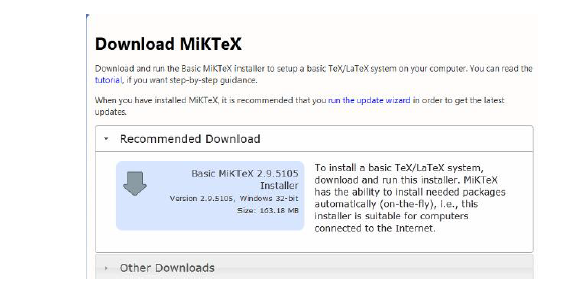
\includegraphics[width =10 cm]{img/18.png}
	\captionof{figure}{Download MikTeX}
	\label{picture label}
\end{center}
\item Setelah software berhasil di download, jalankan software tadi. Akan muncul persetujuan penggunaan MiKTex. Centang {\bf \itshape{I accept the MiKTex copying condition}}, kemudian klik {\bf next}.
\begin{figure}[h!]
    \centering
    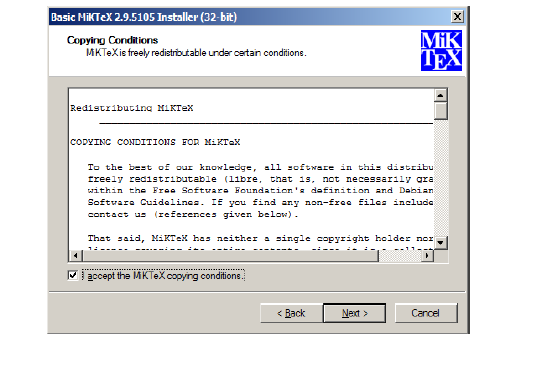
\includegraphics[width =10 cm]{img/19.png}
    \captionof{figure}{MikTeX \textit{pop-up}}
	\label{picture label}
\end{figure}
\newpage
\item Kemudian, akan muncul pilihan untuk siapa saja software ini digunakan. Saran dari penulis klik {\bf Only for nama \itshape User} agar lebih menghemat memory komputer. Kemudian klik {\bf next}.
\begin{figure}[h!]
    \centering
    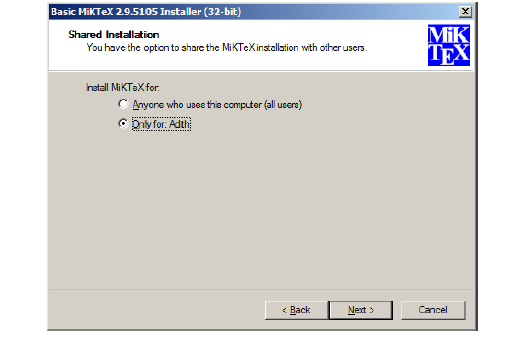
\includegraphics[width =10 cm]{img/20.png}
    \captionof{figure}{MikTeX \textit{pop-up} 2}
	\label{picture label}
\end{figure}
\item Kemudian pilih lokasi untuk penampung software MiKTex. Lalu klik {\bf next}.
\begin{figure}[h!]
    \centering
    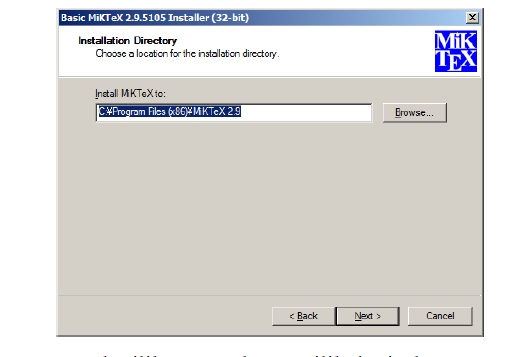
\includegraphics[width =10  cm]{img/21.png}
    \captionof{figure}{MikTeX \textit{pop-up} 3}
	\label{picture label}
\end{figure}
\item Lalu, akan muncul pilihan untuk memilih jenis kertas yang digunakan. Pilih {\bf A4} sebagai jenis kertas dan ask me first. Kemudian klik {\bf next}. Selanjutnya klik {\bf start}.
\newpage
\begin{figure}[h!]
\centering
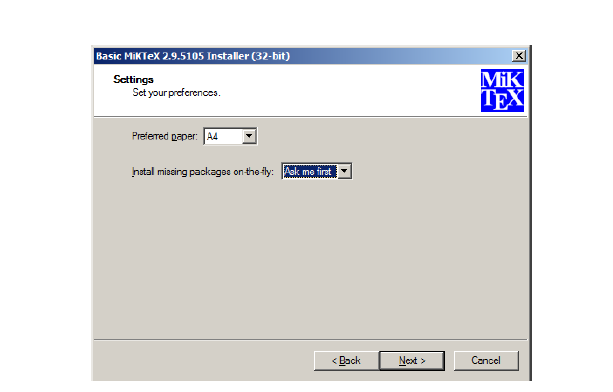
\includegraphics[width =10 cm]{img/22.png}
\end{figure}
\item Tunggu proses instalasi selesai.
\end{enumerate}
LaTex memerlukan teks editor untuk menulis perintah yang akan di eksekusi, serta sebagai compiler dari perintah-perintah tadi. Notepad bawaan windows dapat dijadikan sebagai teks editor. Bila menggunakan notepad, ubah jenis file yang akan disimpan menjadi .tex. Namun untuk para pemula, kami sarankan anda untuk menggunakan software seperti teXstudio, teXworks, ataupun teks editor lainnya yang khusus menangani LaTex. Sebab, software-software tadi menyediakan perintah-perintah yang khusus sehingga memudahkan para pemula untuk belaajr menggunakan LaTex.
\begin{enumerate}
\item {\itshape Download} aplikasi teXstudio di situs {\bf http://texstudio.sourceforge.net/} .
\item Kemudian, klik aplikasi yang telah didownload. Pilih bahasa yang akan digunakan. Kemudian klik {\bf ok}.
\begin{figure}[h!]
\centering
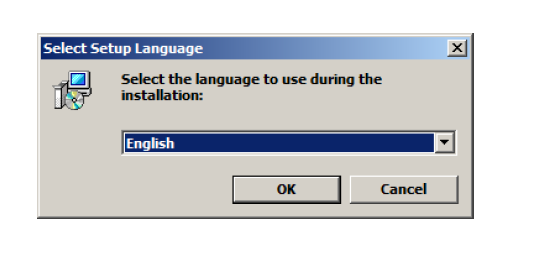
\includegraphics[width =10 cm]{img/23.png}
\end{figure}
\newpage
\item Klik {\bf next} untuk melanjutkan ke proses berikutnya.
\begin{figure}[h!]
\centering
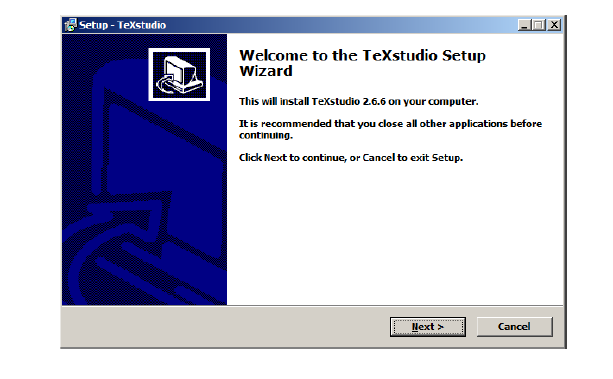
\includegraphics[width =10 cm]{img/24.png}
\end{figure}
\item Klik {\bf browse} untuk memilih lokasi file teXstudio. Setelah memilih lokasinya, klik {\bf next}.
\begin{figure}[h!]
\centering
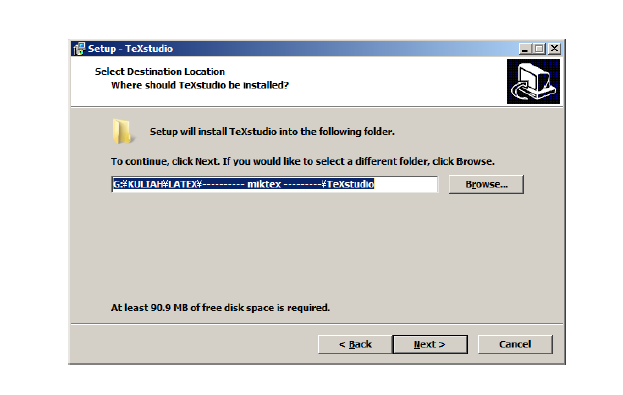
\includegraphics[width =10 cm]{img/25.png}
\end{figure}
\newpage
\item Kemudian akan muncul pilihan untuk memilih tempat folder. Klik {\bf next} untuk melanjutkan proses.
\begin{figure}[h!]
\centering
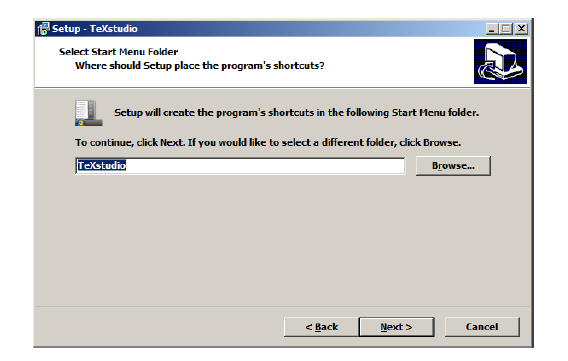
\includegraphics[width =10 cm]{img/26.png}
\end{figure}
\item Klik {\bf install} untuk memulai proses instalasi.
\newpage
\begin{figure}[h!]
\centering
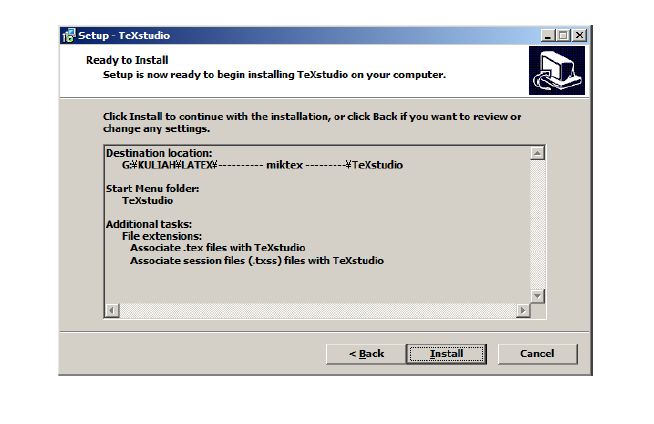
\includegraphics[width =10cm]{img/27.png}
\end{figure}
\item Tunggu proses instalasi selesai.
\end{enumerate}
\section{Perintah-Perintah Dalam  Latex}
\subsection{Format Perintah}
\begin{raggedleft}
Semua perintah Latex diawali dengan tanda backslash (\textbackslash). Tanda ini memberitahukan kepada LATEX untuk melakukan hal tertentu pada bagian dokumen tersebut. Perintah-perintah dalam Latex biasanya sudah cukup menjelaskan apa yang akan dilakukan LATEX pada dokumen kita. Misalnya:\end{raggedleft}
\begin{table}[h!]
\begin{tabular}{ll p{5 cm}}
\bfseries{\textcolor{blue}{\textbackslash tableofcontents}} &:& perintah ini digunakan untuk menambahkan daftar isi sebuah   dokumen.\\
\bfseries{\textcolor{blue}{\textbackslash documentclass}} & :& perintah untuk menentukan jenis dokumen yang akan dibuat  dan harus ada pada awal  dokumen. \\
\bfseries{\textcolor{blue}{\textbackslash bfseries}}&:& perintah untuk menebalkan teks pada dokumen Latex
\end{tabular}
\end{table}
\subsection{Preamble, Dekalarasi \& Environment}
\begin{raggedleft}Yang dimaksud dengan preamble/pembukaan adalah bagian dari dokumen LATEX di antara per-intah \textbackslash  documentclass dan perintah \textbackslash begin{document}. Hanya ada beberapa perintah yang hanya bisa diletakkan di bagian ini. Yang paling umum diletakkan dalam bagian preamble adalah deklarasi penggunaan paket-paket LATEX .\end{raggedleft}
\subsection{Spasi dalam Latex}
\begin{raggedleft}Dalam dokumen LATEX semua baris-baris kosong, spasi yang banyak, dan tabulasi dianggap sebagai 1 spasi atau 1 baris kosong saja selama proses pengaturan tulisan. LATEX mengatur spasi dan perataan teks (alignment) berdasarkan perintah yang diterimanya, sehingga kita mampu mengaturnya secara tepat. Contohnya :\end{raggedleft}
\begin{table}[h!]
\begin{tabular}{|p{5 cm} p{8 cm}|}
\hline
\bfseries{\textcolor{blue}{\textbackslash chapter}}\bfseries{\textcolor{red}{ \{}}Pendahuluan\bfseries{\textcolor{red}{\}}}& \\
ini adalah contoh dokumen &  \\
\hline
\end{tabular}
\end{table}
\\ \begin{raggedleft}Format penulisan di atas akan menghasilkan keluaran yang sama jika dituliskan seperti ini : \end{raggedleft}
\begin{table}[h!]
\begin{tabular}{|p{13.5 cm}|}
\hline
\bfseries{\textcolor{blue}{\textbackslash chapter}}  \bfseries{\textcolor{red}{\{}}Pendahuluan\bfseries{\textcolor{red}{\}}} ini adalah contoh dokumen \\
\hline
\end{tabular}
\end{table}
\\
Ada perintah khusus untuk membuat spasi dengan panjang tertentu baik secara horizontal maupun vertikal, yaitu :
\begin{itemize}
\item Jika kita ingin membuat jarak dengan panjang tertentu antara 2 baris, kita dapat menggunakan tanda ‘ \textbackslash \textbackslash’ di akhir baris. Kita juga dapat menentukan sendiri panjang baris kosong dengan menggunakan perintah seperti contoh berikut ini : 
\begin{table}[h!]
\begin{tabular}{|p{13.5 cm}|}
\hline
\bfseries{\textcolor{red}{baris 1}} \textbackslash  \textbackslash  \\
\bfseries{\textcolor{blue}{\textbackslash vspace \{ }} \bfseries{\textcolor{red}{2 cm}} \textcolor{blue}{ \} } \\
\bfseries{\textcolor{red}{baris 2}} \textbackslash  \textbackslash  \\
\hline
\end{tabular}
\end{table}
\\
Dengan perintah ini LATEX akan membuat mengosongkan baris-baris sepanjang 2 centimeter.Tanpa perintah ini sejauh apapun kita membuat spasi dalam teks dokumen, LATEX akan tetap menganggapnya 1 spasi.
\item Jika kita ingin membuat spasi sejauh beberapa centimeter antara 2 kata dibutuhkan
perintah : \\
\begin{table}[h!]
\begin{tabular}{|p{13.5 cm}|}
\hline
kata 1 \textbackslash hspace\{2cm\} kata 2\\
\hline
\end{tabular}
\end{table}
\\
Dengan perintah ini LATEX akan membuat spasi sejauh 2 centimeter. Sama seperti poin sebelumnya tanpa perintah ini sejauh kita membuat spasi dalam teks dokumen, LATEX akan tetap menganggapnya 1 spasi. \\[0.5 cm]

Jadi secara umum aturan yang dapat dipakai adalah : akhiri paragraf dengan tanda ‘\textbackslash \textbackslash’ dan berikan 1 baris kosong antara tiap-tiap paragraf dan 1 spasi kosong antara masing-masing kata.

\end{itemize}
\subsection{Hyphenation}
hyphenation berfungsi untuk memperbaiki pemenggalan kata yang mungkin kurang tepat, sebagai contohnya  kata “mungkin” dipenggal menjadi kata “mun-gkin”. Berikut adalah contoh penggunaan hyphenation: \\[0.5 cm]
\begin{tabular}{|p{13.5 cm}|}
\hline
\textbackslash usepackage \{hyphenation\} \\
          \textbackslash hyphenation \{mung-kin, sa-ngar, mi-num\}\\

\hline
\end{tabular}
\subsection{Alignment}
Alignmen atau yang disebut dengan perataan baris pada Latex dibagi menjadi 3 jenis yaitu: rata kiri, rata, rata kanan, dan rata tengah. Dokumen pada Latex secara default diatur dengan perataan justified (rata kanan kiri). Berikut adalah contoh penggunaan alignmen pada Latex:
\begin{description}
\item[a.]	Alignment rata kiri\\
\begin{tabular}{|p{12cm}|}
\hline
\textbackslash begin\{raggedright\} \\
    Isi dokumen diatur secara rata kiri \\
  \textbackslash end\{raggedright\} \\
\hline
\end{tabular}
\item[b.] Alignment rata kanan\\
\begin{tabular}{|p{12cm}|}
\hline
\textbackslash begin\{raggedleft\} \\
    Isi dokumen diatur secara rata kanan \\
  \textbackslash end\{raggedleft\} \\
\hline
\end{tabular}
\item[c.]  Alignment  rata tengah\\
\begin{tabular}{|p{12cm}|}
\hline
\textbackslash begin\{center\} \\
    Isi dokumen diatur secara rata tengah \\
  \textbackslash end\{center\} \\
\hline
\end{tabular}
\end{description}
\subsection{Bahasa}
\begin{raggedleft} LATEX dapat mengatur tulisan mengikuti aturan ejaan yang dimiliki beberapa bahasa tertentu. Kemampuan ini diatur oleh babel package yang dimiliki LATEXH˙ al tersebut berpengaruh pada pemenggalan kata, spasi setiap kata, indentasi, dan beberapa judul bagian dokumen yang digunakan dalam heading. Mengubah pengaturan bahasa dengan menggunakan babel akan secara otomatis mengubah nama-nama dari unit struktur dokumen (seperti misalnya Abstract, Chapter, Index) menjadi terjemahannya.\end{raggedleft} \\[0.5 cm]

\begin{raggedleft} Perintah yang mengatur LATEX untuk menggunakan babel bahasa Indonesia adalah seperti berikut ini :\end{raggedleft} \\
\begin{tabular}{|p{13.5cm}|}
\hline
\textbackslash documentclass [a4paper, 12pt]\{report\}\\
\textbackslash usepackage[bahasa]\{babel\}\\
Cara mengatur\\
\textbackslash begin\{document\} bahasa\\
. . . . . . . . . . . . . . . . . .\\
. . . . . . . . . . . . . . . . . .\\
\textbackslash end\{document\}\\
\hline
\end{tabular}
\subsection{Keterangan}
Jika ini menambahkan keterangan pada dokumen Latex (yang tidak akan tercetak). Caranya adalah dengan menambahkan  tanda \textquotedblright \%\textquotedblleft  di awal kata yang akan dijadikan keterangan. Contohnya:\\[0.5 cm]
\begin{tabular}{|p{13.5cm}|}
\hline
 \textbackslash documentclass [a4paper, 12pt]\{report\} \% untuk menentuka ukuran kertas dan huruf\\
\textbackslash  usepackage[bahasa]\{babel\} \% untuk merubah kata kedalam bahasa Indonesia.\\
\textbackslash  begin\{document\}
   \% ini adalah baris keterangan, baris ini tidak akan tercetak pada saat file dijalankan\\
  ……………….
\textbackslash end\{document\}\\

\hline
\end{tabular}
\subsection{Karakter Khusus}
Ada beberapa karakter tertentu yang membutuhkan perintah khusus untuk menuliskannya pada dokumen Latex. Berikut adalah diantaranya:
\begin{longtable}{|l|l|l|l|}
\hline
Karakter&Penulisan&Karakter&Penulisan\\ \hline
\textbackslash & \textbackslash textbackslash& \$ &\textbackslash \$\\ \hline
\%&\textbackslash\%&\^{} & \textbackslash \^{}\{\}\\ \hline
\_&\textbackslash\_&\~{}&\textbackslash \~{}\{\}\\ \hline
\{&\textbackslash\{&\}&\textbackslash\}\\ \hline
\textgreater&\textbackslash textgreater&\textless &\textbackslash textless\\ \hline
\textbar&\textbar& \textquotedblleft& \textbackslash textquotedblleft\\ \hline
\textquotedblright&\textbackslash textquotedblright & \textquoteleft&\textbackslash textquoteleft\\ \hline
\textquoteright&\textbackslash textquoteright&\#& \textbackslash \#\\ \hline
\end{longtable}

\begin{raggedleft} Dalam bahasa asing sering digunakan aksen dan symbol-simbol tertentu dalam penulisan bahasanya. Berikut adalah beberapa aksen dan symbol yang sering digunakannya:\end{raggedleft} \\
\begin{figure}[h!]
\centering
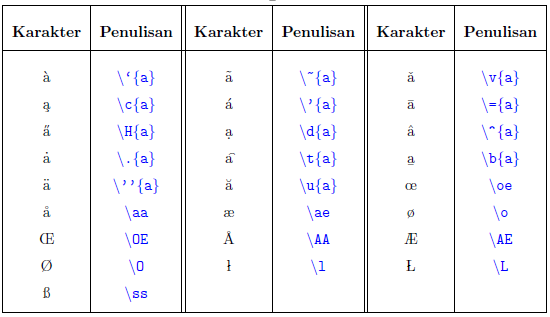
\includegraphics[width = 10cm]{img/1.png}
\end{figure}
\subsection{Font dalam Latex}
\subsubsection{Jenis Font}
Font standar dalam Latex yang disediakan ada 3 jenis yaitu:
\begin{enumerate}
\item Roman, berikut adalah cara menggunakan jenis font di bawah ini:\\
\begin{tabular}{|p{12 cm }|}
\hline
\{ \textbackslash rmfamily teks yang akan diformat\}\\
\hline
\end{tabular}
\item Sans serif, berikut adalah cara menggunakan jenis font di bawah ini:\\
\begin{tabular}{|p{12 cm }|}
\hline
\{ \textbackslash sffamily teks yang akan diformat\}\\
\hline
\end{tabular}
\item Typewriter, berikut adalah cara menggunakan jenis font di bawah ini:\\
\begin{tabular}{|p{12 cm }|}
\hline
\{ \textbackslash ttfamily teks yang akan diformat\}\\
\hline
\end{tabular}
\end{enumerate}
\subsubsection{Bentuk Font}
Bentuk font yang disediakan pada Latex, yaitu:
\begin{enumerate}
\item Italic, cara mengatur bentuk font seperti ini adalah:\\
\begin{tabular}{|p{12 cm }|}
\hline
\{\textbackslash itshape teks yang akan diformat\}\\
\hline
\end{tabular}

\item Slanted,  cara mengatur bentuk font seperti ini adalah:\\
\begin{tabular}{|p{12 cm }|}
\hline
\{\textbackslash slshape teks yang akan diformat\}\\
\hline
\end{tabular}
\item 	Vertical, Cara mengatur bentuk font seperti ini adalah:\\
\begin{tabular}{|p{12 cm }|}
\hline
\{\textbackslash upshape teks yang akan diformat\}\\
\hline
\end{tabular}
\item   Small Caps, cara mengatur bentuk font seperti ini adalah:\\
\begin{tabular}{|p{12 cm }|}
\hline
\{\textbackslash scshape teks yang akan diformat\}\\
\hline
\end{tabular}
\end{enumerate}
\subsubsection{Ukuran Font}
Ada beberapa macam ukuran font yang ada dalam dokumen Latex yaitu:
\begin{figure}[h!]
\centering

\includegraphics[width=  10 cm]{img/2.png}
\end{figure}
\\
Berikut cara menggunakan ukuran-ukuran font tersebut adalah:
\begin{description}
\item[-]Tiny : \{\textbackslash tiny teks yang akan diformat\}
\item[-] Scriptsize : \{\textbackslash scriptsize teks yang akan diformat\}
\item[-] Footnotesize : \{\textbackslash  footnotesize  teks yang akan diformat\}
\item[-] Small : \{\textbackslash small teks yang akan diformat\}
\item[-] Normal :  \{\textbackslash normal teks yang akan diformat\}
\item[-] Large :  \{\textbackslash large teks yang akan diformat\}
\item[-] Larger :  \{\textbackslash Large teks yang akan diformat\}
\item[-] Largest : \{\textbackslash LARGE teks yang akan diformat\}
\item[-] Huge :  \{\textbackslash huge teks yang akan diformat\}
\item[-] Huger :  \{\textbackslash Huge teks yang akan diformat\}
\end{description}
\subsection{Mode Verbatim}
\begin{raggedleft}Mode verbatim berfungsi untuk menampilkan sesuai teks seperti apa yang kita ketik. Pada dasarnya semua dokumen Latex yang ingin ditampilkan pada file keluarannya harus dilengkapi dengan perintah. Untuk menampilkan teks keluaran sesuai apa yang kita ketik maka gunakan mode verbatim.\end{raggedleft}
\vspace{0.5 cm}

\begin{raggedleft}Contoh penulisan tanpa menggunkana mode verbatim:\end{raggedleft}\\
\begin{tabular}{|p{13.5 cm}|}
\hline
Ini adalah baris pertama \\[0.5 cm]


Ini adalah baris kedua     \hspace{0.5 cm}   dari contoh\\
\hline
\end{tabular}\\[0.5 cm]
\vspace{0.5 cm}
Hasil outputnya:\\
\begin{tabular}{|p{13.5 cm}|}
\hline
Ini adalah baris pertama \\


Ini adalah baris kedua  dari contoh\\
\hline
\end{tabular}\vspace{0.5 cm}
\begin{raggedleft}
Pada contoh di atas terlihat seberapa jauhpun kita membuat spasi horizontal atau vertical, hasilnya tidak akan terpengaruh. Hasilnya hanya menampilkan sesuai yang diperintahkan dan menurut standar Latex. Supaya teks yang dihasilkan sama persis susunan dan formasinya seperti apa yang kita ketik, kita bisa menggunakan mode verbatim. Berikut adalah cara penggunaanya:\end{raggedleft} \\[0.5 cm]
\begin{tabular}{|p{13.5 cm}|}
\hline
\textbackslash begin \{verbatim\}\\
Ini adalah baris pertama \\[0.5 cm]


Ini adalah baris kedua     \hspace{0.5 cm}   dari contoh\\
\textbackslash end\{verbatim\} \\
\hline
\end{tabular}\\[0.5 cm]
Hasil outputnya: \\[0.5 cm]
\vspace{0.5 cm}
\begin{tabular}{|p{13.5 cm}|}
\hline
\begin {verbatim}
Ini adalah baris pertama 


Ini adalah baris kedua      dari contoh
\end{verbatim} \\
\hline
\end{tabular}\\[0.5 cm]
Mode verbatim ini sangat cocok digunakan untuk penulisan source code atau dokumentasi pembuatan perangkat lunak.
\section{Struktur Dokumen Latex}
\subsection{Document Class}
Class file pada LATEX menentukan layout halaman, jenis heading, dan berbagai perintah dan environment yang diperlukan untuk mengatur style dokumen. Cara untuk mendeklarasikan Document Class adalah memulai dokumen dengan :\\[0.5 cm]
\begin{tabular}{|p{13.5 cm}|}
\hline
\textbackslash documentclass\{class\}\\
\hline
\end{tabular}\\[0.5 cm]
Ada beberapa jenis document class yang bisa dipakai dalam sebuah dokumen, yaitu :
\begin{itemize}
\item {\bf report} : kelas ini dapat digunakan untuk membuat laporan (report) baik dalam bidang
bisnis, teknik, hukum, akademis, atau ilmu pengetahuan.
\item  {\bf article} : kelas ini dapat digunakan untuk membuat paper, artikel sebuah jurnal atau
majalah, review, paper untuk konferensi, atau catatan riset.
\item {\bf book} : kelas ini digunakan untuk membuat buku dan thesis.
\item {\bf letter} : kelas ini digunakan untuk membuat surat.
\end{itemize}
Biasanya kelas ‘article’ adalah yang paling sering digunakan untuk sembarang jenis dokumen. Masing-masing kelas di atas memiliki strukturnya sendiri. Misalnya pada kelas article tidak ada elemen bab, tidak seperti pada kelas report dan book.\\[0.5 cm]
\vspace{0.5 cm}
Secara sederhana struktur dokumen  Latex adalah sebagai berikut:\\
\begin{tabular}{|p{13.5 cm}|}
\hline
\textbackslash documentclass\{. . .\}\\
\textbackslash begin\{document\}\\
      Bagian isi dokumen\\
\textbackslash end\{document\}\\
\hline
\end{tabular}
\subsection{Document Class Option}
Document Class Option maksudnya adalah pilihan yang tersedia pada kelas dokumen yang bisa kita tentukan sendiri isinya. Opsi pada suatu kelas dokumen dituliskan seperti berikut :\\[0.5 cm]
\begin{tabular}{|p{13.5 cm}|}
\hline
          \textbackslash documentclass [ option1, option2 ] \{ class \}\\
\hline
\end{tabular}\\[0.5 cm]
Seperti terlihat di atas, kita dapat menentukan beberapa opsi sekaligus dalam tanda kurung dengan dibatasi tanda koma.\\[0.5 cm]

\begin{raggedleft}Default opsi yang digunakan oleh LATEX antara lain :\end{raggedleft}

\begin{itemize}
\item Ukuran kertas yang digunakan adalah A4.
\item Ukuran font yang digunakan adalah 10pt untuk semua kelas dokumen.
\item Layout halaman yang digunakan adalah two-sided printing khusus untuk kelas book dan report, dan one-sided printing khusus untuk kelas article dan letter.
\item  Halaman judul yang terpisah di bagian awal dokumen khusus untuk kelas book dan
report.
\end{itemize}
Opsi di atas dapat modifikasi dengan beberapa opsi berikut :
\begin{itemize}
\item Ukuran kertas : Kita dapat menentukan sendiri ukuran kertasnya. Cara penulisannya:\\[0.5 cm]
\begin{tabular}{|p{12 cm}|}
\hline
\textbackslash documentclass [ a3paper ] \{ class \} atau \\
\textbackslash documentclass [ letterpaper ] \{ class \}\\
\hline
\end{tabular}
\item Ukuran font : kita dapat memilih ukuran 10pt, 11pt, atau 12pt. Cara penulisannya :\\[0.5 cm]
 \begin{tabular}{|p{12 cm}|}
\hline
\textbackslash documentclass [ a4paper, 11pt ] \{class\}\\
\hline
\end{tabular}\\[0.5 cm]
Setelah kita menentukan ukuran font yang dipakai, semua font dalam dokumen akan diatur sedemikan sehingga memiliki ukuran sesuai dengan yang kita tentukan. Font yang dipakai pada header, footer disesuaikan secara proporsional dengan ukuran font tersebut.
\item Layout halaman dapat kita tentukan sendiri dengan 2 pilihan berikut :
\begin{itemize}
\item[-] oneside : jika kita menginginkan layout one-sided printing saat menggunakan kelas book dan report.
\item[-] twoside : jika kita menginginkan layout two-sided printing saat menggunakan kelas  article.
\item[-] titlepage : jika kita menginginkan kelas article untuk memiliki halaman judul yang          terpisah di bagian awal dokumen.
\item[-]draft : opsi ini mengatur LATEX supaya menandai masalah-masalah yang timbul seperti masalah pemenggalan kata (pemenggalan kata tidak tepat) atau masalah perataan tulisan (ada baris tertentu yang melebihi batas kanan dokumen). Tanda yang akan digunakan LATEX adalah sebuah persegi kecil di bagian kanan dokumen tempat terjadinya masalah.
\end{itemize}
\end{itemize}
\section{Paket (Package)}
Yang dimaksud dengan paket dalam LATEX adalah fungsi-fungsi yang dipakai untuk menambah kemampuan LATEX melakukan pengaturan dokumen. Ada banyak sekali paket yang dimiliki LATEX baik yang sudah terintegrasi bersamaan di dalam instaler LATEX maupun yang belum. Paket-paket yang belum terinstal bisa didownload dari http://www.ctan.org. Untuk menggunakan paket tertentu dalam dokumen yang kita buat, kita perlu mendeklarasikannya terlebih dulu pada bagian preamble1. Cara menggunakan paket yang sudah tersedia/terintegrasi di dalam LATEX adalah seperti ini :\\[0.5 cm]
\begin{tabular}{|p{13.5 cm}|}
\hline
\textbackslash documentclass \{class\}\\
\textbackslash usepackage [ option ] \{nama paket\}\\\
\textbackslash begin\{document\}\\
. . . . . . . . . . . . . . . . . .\\
. . . . . . . . . . . . . . . . . .\\
. . . . . . . . . . . . . . . . . .\\
\textbackslash end\{document\}\\
\hline

\end{tabular}\\[0.5 cm]
Beberapa paket yang terintegrasi dalam LATEX antara lain :
\begin{enumerate}
\item	graphicx : paket ini membuat LATEX mampu menghasilkan gambar grafis dan juga membuat LATEX mampu menampilkan gambar yang kita sertakan dalam dokumen.
\item	hyperref : paket ini membuat LATEX mampu menghasilkan dokumen yang memiliki dynamic link2 ke alamat tertentu.
\item babel : paket ini membuat LATEX mampu mengenali format bahasa yang digunakan
\item	seperti yang sudah dijelaskan pada subbab Bahasa di Bab Perintah-Perintah LATEX .
\item	color : paket ini membuat LATEX mampu menghasilkan teks dokumen yang memiliki warna sesuai warna yang ditentukan.
\item	makeidx : paket ini membuat LATEX mampu menghasilkan indeks dari dokumen yang dibuat.
\end{enumerate}
\section{Document Enviroment}
Yang dimaksud dengan document environment adalah bagian dalam sebuah dokumen LATEX dimana isi sebenarnya dari dokumen itu sendiri ditempatkan.\\[0.5 cm]
\begin{tabular}{|p{13.5 cm}|}
\hline
\textbackslash documentclass\{class\}\\
\textbackslash begin\{document\}\\\
. . . . . . . . . . . . . . . . . .\\
. . . . . . . . . . . . . . . . . .\\
. . . . . . . . . . . . . . . . . .\\
\textbackslash end\{document\}\\
\hline

\end{tabular}\\[0.5 cm]
Semua teks isi dari dokumen harus dituliskan di bagian titik-titik tersebut di atas. Teks yang ditulis sebelum \textbackslash begin\{document\} dan sesudah \textbackslash end\{document\}, kelak tidak akan muncul pada dokumen hasil compile. Struktur \textbackslash begin . . . \textbackslash end inilah yang disebut dengan environment. Environment membatasi bagian teks yang akan diatur dengan aturan tertentu. Bagian antara deklarasi kelas dokumen dengan awal document environment disebut preamble.
\section{Penulisan Judul}
Judul dalam sebuah dokumen latex diletakan pada awal document environment, Cara penulisannya sebagai berikut:\\[0.5 cm]
\begin{tabular}{|p{13.5 cm}|}
\hline
\textbackslash documentclass [a4paper, 12pt]\{report\}\\
\textbackslash begin\{decument\}\\
        \textbackslash titile\{Judul Document\}\\
        \textbackslash autor\{Nama Penulis\}\\
        \textbackslash date\{Tanggal Pembuatan\}\\
        \textbackslash maketitle\\
. . . . . . . . . . . . . . . .\\
. . . . . . . . . . . . . . . . \\
\textbackslash end\{document\}\\

\hline

\end{tabular}\\[0.5 cm]
\section{Abstrak}
Pada dokumen kelas article dan report umumnya memiliki abstrak/ringkasan. Latex memiliki cara khusus untuk menuliskan abstrak. Berikut adalah cara penulisannya:\\
\begin{tabular}{|p{13.5 cm}|}
\hline
 \textbackslash  documentclass [a4paper, 12pt]\{report\}\\
 \textbackslash  begin\{decument\} \\
         \textbackslash  titile\{Judul Document\} \\
         \textbackslash  autor\{Nama Penulis\} \\
         \textbackslash  date\{Tanggal Pembuatan\}\\
         \textbackslash maketitle \\

         \textbackslash begin\{abstract\}\\
             Isi abstrak\\
         \textbackslash end\{abstract\}\\
. . . . . . . . . . . . . . . . \\
\textbackslash end\{document\}\\

\hline

\end{tabular}\\[0.5 cm]
\begin{raggedleft}Jika ingin mengubah judul abstrak digunakan perintah ini sebelum \end{raggedleft}\\  \textbackslash begin\{abstract\}:\\[0.5 cm]
\begin{tabular}{|p{13.5 cm}|}
\hline
\textbackslash renewcommand\{\textbackslash abstractname\}\{RINGKASAN LAPORAN\}\\
\hline
\end{tabular}\\[0.5 cm]
Perintah di atas akan mengganti judul abstrak menjadi \textquotedblleft RINGKASAN LAPORAN \textquotedblright
\section{Sistematika Isi Dokumen}
\begin{raggedleft} LATEX memiliki kemampuan untuk membagi dokumen dalam suatu susunan struktural (bab, subbab, subsubbab, dst) sampai 7 tingkatan. Berikut adalah daftar struktur yang disediakan dalam latex:\end{raggedleft}\\[0.5 cm]
\begin{tabular}{|p{10 cm}|p{3.5 cm}|}
\hline
Struktur&Perintah\\ \hline
Bagian (Part)&\textbackslash part\{...\}\\
Bab (Chapter)&\textbackslash chapter\{...\}\\
Subbab (Section)&\textbackslash section\{...\}\\
Subsubbab (subsubsection)&\textbackslash subsection\{...\}\\
Subsubsubbab (subsubsection)&\textbackslash subsubsection\{...\}\\
Paragraf berjudul (titled paragraph)&\textbackslash paragraph\{...\}\\
Anak paragraph berjudul (titled subparagraph)&\textbackslash subparagraph\{...\}\\
\hline
\end{tabular}\\[0.5 cm]
Ada beberapa hal yang perlu diketahui tentang penggunaan struktur di atas :\\
\begin{itemize}
\item Hanya dokumen dengan kelas book dan report bisa menggunakan semua struktur di atas.
\item  Dokumen kelas article hanya bisa menggunakan kelas \textbackslash section\{...\} dan struktur di bawahnya bawah.
\item  Dokumen kelas letter tidak dapat menggunakan semua struktur di atas.
\end{itemize}
Contoh penggunaanya adalah sebagai berikut:\\
\begin{tabular}{|p{13.5 cm}|}
\hline
\textbackslash documentclass [a4paper, 12pt] \{report\}\\
\textbackslash begin\{document\}\\
   \textbackslash title\{Judul Dokumen\}\\
    \textbackslash author\{Nama Penulis\}\\
    \textbackslash date\{Tanggal Pembuatan\}\\
    \textbackslash maketitle\\

       \textbackslash begin\{abstract\}\\
          isi abstract\\
       \textbackslash end\{abstract\}\\

        \textbackslash chapter\{Pendahuluan\}\\
           isi bab I pendahuluan\\
         \textbackslash section\{Latar Belakang\}\\
           isi subbab latar belakang\\

          \textbackslash chapter\{Dasar Teori\}\\
              isi bab II dasar teori\\
          \textbackslash section\{Tinjauan Pustaka\}\\
              isi subbab tinjauan pustaka\\

\textbackslash end\{document\}\\
\hline
\end{tabular}
\section{Daftar Berurut }
Ada 3 Jenis cara penulisan daftar berurut yaitu:
\begin{enumerate}
\item Daftar dengan penomoran menggunakan simbol (Bulleted List), contohnya seperti
berikut ini :
\begin{itemize}
\item Apel
\item Jeruk 
\item Semangka
\item Durian
\end{itemize}
Format penulisan daftar seperti ini adalah sebagai berikut :\\[0.5 cm]
\begin{tabular}{|p{12.5 cm}|}
\hline
\textbackslash begin\{itemize\}\\
\textbackslash item . . .\\
\textbackslash item . . .\\
\textbackslash item . . .\\
. . . .\\
\textbackslash end\{itemize\}\\

\hline
\end{tabular}\\[0.5 cm]
Isi daftar dituliskan setelah \textbackslash item. Simbol yang dipakai dapat kita tentukan sendiri.
Sebagai contoh jika kita ingin menggunakan tanda * sebagai penanda item, caranya adalah dengan menambahkan keterangan simbol yang digunakan seperti berikut : \textbackslash item[*] ...
\item Daftar dengan penomoran menggunakan angka (Numbered List), contohnya seperti berikut ini :\\
\begin{enumerate}
\setlength{\itemindent}{-0.1 in}
\setlength\itemsep{0 em}
\item[1.] Apel
\item[2.] Jeruk 
\item[3.] Semangka
\item[4.] Durian
\end{enumerate}
Format penulisan daftar seperti ini adalah sebagai berikut :\\[0.5 cm]
\begin{tabular}{|p{12.5 cm}|}
\hline
\textbackslash begin\{enumerate\}\\
\textbackslash item . . .\\
\textbackslash item . . .\\
\textbackslash item . . .\\
. . . .\\
. . . .\\
\textbackslash end\{enumerate\}\\

\hline
\end{tabular}
\item Daftar deskripsi, contohnya seperti berikut ini :
\begin{description}
\item[ITB]Institut Teknologi Bandung
\item[UI]Universitas Indonesia
\item[IPB]Institut Pertanian Bogor
\item[UGM]Universitas Gajah Mada
\end{description}
Cara penulisannya adalah seperti berikut ini :\\[0.5 cm]
\begin{tabular}{|p{12.5 cm}|}
\hline
\textbackslash begin\{description\}\\
\textbackslash item[ Hal 1 ] penjelasan hal 1\\
\textbackslash item[ Hal 2 ] penjelasan hal 2\\
\textbackslash item[ Hal 3 ] penjelasan hal 3\\
\textbackslash item[ Hal 4 ] penjelasan hal 4\\
. . . .\\
. . . .\\
\textbackslash end\{description\}\\

\hline
\end{tabular}
\end{enumerate}
\section{Daftar isi}
Untuk menampilkan daftar isi digunakan perintah :\\[0.5 cm]

\textbackslash tableofcontents\\[0.5 cm]


\begin{raggedleft}Perintah ini diletakkan pada bagian dimana daftar isi tersebut akan ditempatkan. Biasanya daftar isi ditempatkan tepat setelah abstrak/kata pengantar.\end{raggedleft}\\[0.5 cm]


\begin{raggedleft} Untuk menampilkan daftar gambar digunakan perintah :\end{raggedleft}\\[0.5 cm]



\textbackslash listoffigures \\[0.5 cm]


\begin{raggedleft} Untuk menampilkan daftar tabel digunakan perintah :\end{raggedleft}\\[0.5 cm]



\textbackslash listoftables\\[0.5 cm]


\begin{raggedleft} LATEX menghasilkan file berekstensi *.toc untuk menangani daftar isi, daftar gambar, dan daftar tabel. Jika daftar isi, daftar gambar, dan daftar tabel tidak menampilkan keseluruhan struktur dokumen dengan benar, kita dapat mengatur sendiri isinya dengan cara menambahkan perintah-perintah berikut :\end{raggedleft}\\[0.5 cm]



\textbackslash addcontentsline\{toc\}\{struktur\}\{teks yang ingin ditampilkan pada daftar isi\}\\[0.5 cm]


\begin{raggedleft} Struktur dapat diisi dengan chapter, section, subsection, dst, tergantung bagian dokumen yang ingin kita masukkan ke dalam daftar isi. Dengan perintah di atas LATEX akan menghasilkan baris baru dalam daftar isi dan akan secara otomatis menentukan nomor halaman bagian tersebut.\end{raggedleft}
\section{Tabel}
\subsection{Tabel}
Untuk menempatkan sebuah tabel dalam dokumen LATEX caranya adalah menggunakan table environment :\\[0.5 cm]
\begin{tabular}{|p{13.5 cm}|}
\hline
\textbackslash begin\{table\}\\
...\\
\textbackslash end\{table\}\\
\hline
\end{tabular}\\[0.5 cm]
Bagian titik-titik tersebut adalah bagian isi dari tabel itu sendiri. Cara mengisi bagian tersebut adalah seperti berikut :\\[0.5 cm]
\begin{tabular}{|p{13.5 cm}|}
\hline
\textbackslash begin\{center\} 
\textbackslash begin\{tabular\}\{\textbar c\textbar l\textbar r\textbar\}
\textbackslash hline\\
Judul Kolom 1 \& Judul Kolom 2 \& Judul Kolom 3 \\
\textbackslash hline\\
Isi Baris 1 Kolom 1 \& Isi Baris 1 Kolom 2 \& Isi Baris 1 Kolom 3 \\
Isi Baris 2 Kolom 1 \& Isi Baris 2 Kolom 2 \& Isi Baris 2 Kolom 3 \\
\textbackslash hline\\
\textbackslash end\{tabular\}\\
\textbackslash caption\{Contoh Tabel\}\\
\textbackslash end\{center\}\\
\hline
\end{tabular}\\[0.5 cm]
Hasil dari perintah tersebut adalah sebagai berikut :\\[0.5 cm]
\begin{center} 
\begin{tabular}{|c|l|r|}
\hline
Judul Kolom 1 & Judul Kolom 2 & Judul Kolom 3 \\
\hline
Isi Baris 1 Kolom 1 & Isi Baris 1 Kolom 2 & Isi Baris 1 Kolom 3 \\
Isi Baris 2 Kolom 1 & Isi Baris 2 Kolom 2 & Isi Baris 2 Kolom 3 \\
\hline
\end{tabular}

\end{center}
Ada beberapa hal yang perlu diketahui dari format perintah tersebut di atas :\\
\begin{itemize}
\item {\textbar c\textbar l\textbar r\textbar} adalah bagian yang menentukan banyaknya kolom yang akan dihasilkan.    Huruf huruf tersebut mewakili center, left, \& right, yaitu menentukan alignment dari isi sel yang dibuat. Sementara garis — menentukan apakah tabel ingin dibatasi garis atau tidak. Jika antara kolom maupun tidak ingin diberi garis batas, kita tinggal menghilangkan — tersebut.
\item  Pengaturan posisi tabel dapat kita tentukan menurut 2 hal :
\begin{itemize}
	  \item[-] Perataan terhadap tepi dokumen : Dengan mengubah \textbackslash begin\{center\} dan juga
 	     \textbackslash end\{center\} kita bisa menentukan posisi tabel terhadap tepi dokumen.
 	  \item[-] Huruf-huruf pada \textbackslash begin\{table\}[htbp] juga berfungsi sebagai pengatur posisi tabel
                   pada suatu halaman.
\end{itemize}
	\begin{itemize}
	  \item[*] h : tabel diletakkan persis di tempat perintah tersebut dituliskan dalam     dokumen.
	\item[*]  t  : tabel diletakkan di bagian atas halaman.
	\item[*]  b : tabel diletakkan di bagian bawah halaman.
	\item[*]  p : tabel diletakkan pada sebuah halaman khusus yang memuat hanya tabel itu saja.
	\end{itemize}
\item  Untuk menuliskan isi dari masing-masing baris, digunakan format
isi kolom 1 \& isi kolom 2 \& isi kolom 3 dst
Perpindahan kolom saat mengisi sebuah baris ditandai dengan tanda \& .

\item Garis mendatar pada tabel (batas tiap baris) dihasilkan dengan perintah \textbackslash hline
\end{itemize}
\subsection{Long Tabel}
\begin{raggedleft}Long table berfungsi untuk membuat table yang lebih dari satu halaman. Jika anda ingin membuat table dengan isi table yang banyak dan tidak cukup pada satu halaman maka gunakanlah perintah long table.\end{raggedleft}\\

\begin{raggedleft}Berikut adalah cara penggunaan long table dengan menggunakan \end{raggedleft}   \textbackslash usepackage\\ \{longtable\}: \\[0.5 cm]
\begin{tabular}{|p{13.5 cm}|}
\hline
\textbackslash begin\{center\}\\
\textbackslash begin\{longtable\}\{\textbar l\textbar l\textbar l\textbar\}\\
\textbackslash  caption\{contoh table\} \textbackslash\textbackslash \\
    Isi tabel.. \\
    . . . .\\
\textbackslash end\{longtable\}\\
\hline
\end{tabular}\\

\begin{small}
\begin{longtable}[c]{|r|l|r|r|r|l|}
\caption{\textit{Nama tabel}} 
\label{tabel-label}\\
\hline
\multicolumn{1}{|c|}{\textbf{aaa}} &
  \multicolumn{1}{c|}{\textit{\textbf{bbb}}} &
  \multicolumn{1}{c|}{\textbf{ccc}} &
  \multicolumn{1}{c|}{\textbf{ddd}} &
  \multicolumn{1}{c|}{\textbf{eee}} &
  \multicolumn{1}{c|}{\textbf{fff}} \\ \hline
\endhead

1   & Ei utroque electram & 0  & 0  & 10 & Laudem  \\ \hline
2   & Ei utroque electram & 3  & 0  & 7  & Laudem  \\ \hline
3   & Ei utroque electram & 2  & 0  & 8  & Laudem  \\ \hline
4   & Ei utroque electram & 0  & 3  & 7  & Laudem  \\ \hline
5   & Ei utroque electram & 10 & 0  & 0  & Laudem  \\ \hline
6   & Ei utroque electram & 0  & 0  & 10 & Laudem  \\ \hline
7   & Ei utroque electram & 3  & 0  & 7  & Laudem  \\ \hline
8   & Ei utroque electram & 2  & 0  & 8  & Laudem  \\ \hline
9   & Ei utroque electram & 0  & 3  & 7  & Laudem  \\ \hline
10   & Ei utroque electram & 10 & 0  & 0  & Laudem  \\ \hline
11   & Ei utroque electram & 0  & 0  & 10 & Laudem  \\ \hline
12   & Ei utroque electram & 3  & 0  & 7  & Laudem  \\ \hline
13   & Ei utroque electram & 2  & 0  & 8  & Laudem  \\ \hline
14   & Ei utroque electram & 0  & 3  & 7  & Laudem  \\ \hline
15   & Ei utroque electram & 10 & 0  & 0  & Laudem  \\ \hline
16   & Ei utroque electram & 0  & 0  & 10 & Laudem  \\ \hline
17   & Ei utroque electram & 3  & 0  & 7  & Laudem  \\ \hline
18   & Ei utroque electram & 2  & 0  & 8  & Laudem  \\ \hline
19   & Ei utroque electram & 0  & 3  & 7  & Laudem  \\ \hline
20   & Ei utroque electram & 10 & 0  & 0  & Laudem  \\ \hline
21   & Ei utroque electram & 0  & 0  & 10 & Laudem  \\ \hline
22   & Ei utroque electram & 3  & 0  & 7  & Laudem  \\ \hline
23   & Ei utroque electram & 2  & 0  & 8  & Laudem  \\ \hline
24   & Ei utroque electram & 0  & 3  & 7  & Laudem  \\ \hline
25   & Ei utroque electram & 10 & 0  & 0  & Laudem  \\ \hline
26   & Ei utroque electram & 0  & 0  & 10 & Laudem  \\ \hline
27   & Ei utroque electram & 3  & 0  & 7  & Laudem  \\ \hline
28   & Ei utroque electram & 2  & 0  & 8  & Laudem  \\ \hline
29   & Ei utroque electram & 0  & 3  & 7  & Laudem  \\ \hline
30   & Ei utroque electram & 10 & 0  & 0  & Laudem  \\ \hline
31   & Ei utroque electram & 0  & 0  & 10 & Laudem  \\ \hline
32   & Ei utroque electram & 3  & 0  & 7  & Laudem  \\ \hline
33   & Ei utroque electram & 2  & 0  & 8  & Laudem  \\ \hline
34   & Ei utroque electram & 0  & 3  & 7  & Laudem  \\ \hline
35   & Ei utroque electram & 10 & 0  & 0  & Laudem  \\ \hline
36   & Ei utroque electram & 0  & 0  & 10 & Laudem  \\ \hline
37   & Ei utroque electram & 3  & 0  & 7  & Laudem  \\ \hline
38   & Ei utroque electram & 2  & 0  & 8  & Laudem  \\ \hline
39   & Ei utroque electram & 0  & 3  & 7  & Laudem  \\ \hline
40   & Ei utroque electram & 10 & 0  & 0  & Laudem  \\ \hline

\end{longtable}
\end{small}

\subsection{Multiple column Table}
Berfungsi sebagai merge untuk column (kolom) pada table. Berikut adalah contoh penggunaan multi-column:\\[0.5 cm]
\begin{tabular}{|p{13.5 cm}|}
\hline
\textbackslash documentclass[11pt]\{article\}\\
\textbackslash begin\{document\}\\


 \textbackslash begin\{table\}[ht]\\
\textbackslash begin\{center\}\\
\textbackslash begin\{tabular\}\{c\textbar c\}\\
    \textbackslash  hline \\
    \textbackslash  multicolumn\{2\}\{c\}\{Multi-column\}\textbackslash\textbackslash \textbackslash hline \\ 
    X\&X\textbackslash \textbackslash \\
    \textbackslash hline \\
\textbackslash end\{tabular\}\\
\textbackslash end\{center\}\\
\textbackslash end\{table\}\\
\textbackslash end\{document\}\\
\hline
\end{tabular}\\[0.5 cm]

Hasil dari code di atas:\\[0.5 cm]

\begin{table}[ht]
\begin{center}
\begin{tabular}{c|c}
    \hline
    \multicolumn{2}{c}{Multi-column}\\ \hline
    X&X\\
    \hline
\end{tabular}
\end{center}
\end{table}
 \subsection{Multiple Rows Table}
Berfungsi sebagai merge untuk row (baris) pada table. Berikut adalah contoh penggunaan multi-rows:\\[0.5 cm]
\begin{tabular}{|p{13.5 cm}|}
\hline
\textbackslash documentclass[11pt]\{article\}\\
\textbackslash usepackage\{multirow\}\\
\textbackslash begin\{document\}\\

 \textbackslash begin\{table\}[ht]\\
\textbackslash begin\{center\}\\
\textbackslash begin\{tabular\}\{c\textbar c\}\\
    \textbackslash  hline \\
    \textbackslash  multirow\{2\}\{*\}\{Multirow\}\&X \textbackslash\textbackslash \\
    \&X\textbackslash \textbackslash \\
    \textbackslash hline \\
\textbackslash end\{tabular\}\\
\textbackslash end\{center\}\\
\textbackslash end\{table\}\\
\textbackslash end\{document\}\\
\hline
\end{tabular}\\[0.5 cm]
Hasil dari code di atas:\\[0.5 cm]

\begin{table}[ht]
\begin{center}
\begin{tabular}{c|c}
    \hline
    \multirow{2}{*}{Multirow}&X\\ 
    &X\\
    \hline
\end{tabular}
\end{center}
\end{table}
\section{Gambar}
Agar LATEX dapat menempatkan gambar di dalam dokumen, kita perlu mendeklarasikan penggunaan paket graphicx pada bagian preamble. Cara deklarasinya adalah :\\[0.5 cm]

\textbackslash usepackage\{graphicx\}\\[0.5 cm]

\begin{raggedleft}Untuk menempatkan sebuah gambar dalam dokumen LATEX caranya adalah sebagai berikut :\end{raggedleft}\\[0.5 cm]
\begin{tabular}{|p{13.5 cm}|}
\hline
\textbackslash begin\{figure\}[htbp]\\
\textbackslash caption\{Nama Gambar\}\\
    \textbackslash begin\{center\}\\
\textbackslash includegraphics[width=3cm,height=3cm\textbackslash columnwidth]\{nama file gambar\}\\
    \textbackslash end\{center\}\\
\textbackslash end\{figure\}\\
    \hline
\end{tabular}\\[0.5 cm]
Ada beberapa hal yang perlu diketahui dari format perintah di atas :
\begin{itemize}
\item Panjang dan Lebar dari gambar yang akan ditampilkan dapat diubah sesuai keinginan
kita. Isi dari width dapat kita isi dengan lebar gambar tersebut dan isi dari height dapat
kita isi dengan tinggi gambar tersebut; keduanya harus dilengkapi dimensi dari ukuran
panjang yang kita gunakan. Dengan mengatur width dan height kita bisa memasukkan
gambar meskipun gambar tersebut memiliki ukuran dimensi yang besar.
\item File gambar yang ingin kita masukkan dalam dokumen, harus diletakkan pada direktori
yang sama dengan direktori file dokumen (*.tex) kita berada.
\item Pengaturan posisi gambar dapat kita tentukan menurut 2 hal :
-	Perataan terhadap tepi dokumen : Dengan mengubah \textbackslash begin\{center\} dan juga \textbackslash end\{center\} kita bisa menentukan posisi gambar terhadap tepi dokumen.
\end{itemize}
\noindent - Huruf-huruf pada \textbackslash begin\{figure\}[htbp] juga berfungsi sebagai pengatur posisi gambar pada suatu halaman.
\begin{itemize}
\item  h : gambar diletakkan persis di tempat perintah tersebut dituliskan dalam dokumen.
\item	t : gambar diletakkan di bagian atas halaman.
\item	b : gambar diletakkan di bagian bawah halaman.
\item	p : gambar diletakkan pada sebuah halaman khusus yang memuat hanya gambar itu saja.
\end{itemize}
Saat menggunakan h, LATEX akan secara otomatis menempatkan gambar di halaman baru jika tidak ada cukup ruang untuk gambar tersebut di tempat perintah gambar dituliskan.
\section{Hyperref}
Paket ini berfungsi untuk membuat setiap hyperlink yang ada di dokumen menjadi dapat di-klik. Secara default, jika memasukkan alamat URL sebuah website, LATEX akan menganggap itu seperti teks yang lain.
Selain itu, paket hyperref ini juga dapat digunakan untuk merubah bagian daftar isi menjadi clickable. Penggunaan:\\[0.5 cm]
\begin{tabular}{|p{13.5 cm}|}
\hline
\textbackslash usepackage[colorlinks=true,linkcolor=red]\{hyperref\}\\
\hline
\end{tabular}\\[0.5 cm]
Keterangan: \\
Opsi argumen colorlinks=true dan linkcolor=red membuat link menjadi berwarna merah. Anda dapat mengganti warna ini sesuai selera.\\[0.5 cm]
\noindent Paket ini juga berguna untuk membuat referensi secara otomatis ke bagian lain dari dokumen Anda. Sebagai contoh Anda ingin membuat referensi ke bagian Preamble. Tanpa paket hyperref, Anda hanya akan mendapatkan nomor dari bagian yang Anda tuju, jadi semisal bagian Preamble bernomor 2.2, maka ketika Anda mengetikkan perintah \ref{preamble} hanya akan mendapat 2.2. Dengan hyperref, Anda dapat menunjuk pada nama bagian dengan mengetikkan perintah:\\[0.5 cm]
\begin{tabular}{|p{13.5 cm}|}
\hline
\textbackslash nameref\{preamble\}\\
\hline
\end{tabular}\\[0.5 cm]
Perlu diingat bahwa sistem referensi seperti ini dapat dijalankan jika Anda memberi label terlebih dahulu pada bagian yang dituju. Caranya cukup tambahkan perintah \textbackslash label\{namalabel\}. Contoh:\\[0.5 cm]
\begin{tabular}{|p{13.5 cm}|}
\hline
\textbackslash section\{Preamble\}\\
\textbackslash  label\{preamble\}\\

\hline
\end{tabular}
\section{Indentfirst}
Secara default, LATEX mengatur paragraf pertama di tiap section tanpa indent. Sementara standar penulisan di Indonesia, setiap paragraf baru harus mempunyai indent di baris yang pertama. Untuk mengatasi itu, LATEX menyediakan paket yang bernama indentfirst yang berguna untuk membuat semua paragraf ber-indent. Tambahkan bagian berikut di baris Preamble: \\[0.5 cm]
\begin{tabular}{|p{13.5 cm}|}
\hline
\textbackslash usepackage\{indentfirst\}\\

\hline
\end{tabular}
\section{fancyhdr}
fancyhdr berfungsi untuk membuat garis melintang horizontal di setiap halaman. Berikut adalah contoh penggunaan fancyhdr:\\[0.5 cm]
\begin{tabular}{|p{13.5 cm}|}
\hline
\textbackslash usepackage\{fancyhdr\} \\
   \textbackslash pagestyle\{fancy\}\\
    \textbackslash chead\{\} \\
    \textbackslash rhead\{\textbackslash thepage\} \\
\textbackslash lhead\{\textbackslash Latex\textbackslash for Thesis\}\\ 
    \textbackslash rfoot\{\} \\
     \textbackslash lfoot\{\} \\
     \textbackslash cfoot\{\}\\
\hline
\end{tabular}\\[0.5 cm]
Hasil outputnya :\\
\begin{figure}[h!]
\centering
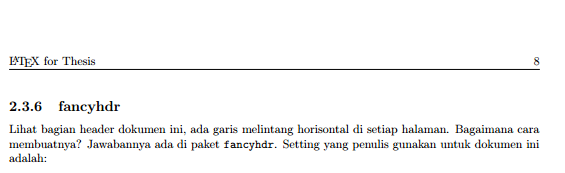
\includegraphics[width=10 cm]{img/6.png}
\end{figure}\\[0.5 cm]
Apabila Anda ingin menghilangkan garis horisontal pada bagian atas dan menggantinya dengan garis horisontal di bagian bawah, caranya:\\[0.5 cm]
\begin{tabular}{|p{13.5 cm}|}
\hline
 \textbackslash usepackage{fancyhdr}\\ 
 \textbackslash pagestyle{fancy} \\
   \textbackslash chead\{\} \\
   \textbackslash rhead\{\}  \\
   \textbackslash lhead\{\} \\
   \textbackslash rfoot\{\} \\
   \textbackslash lfoot\{\} \\
   \textbackslash cfoot\{\textbackslash thepage\}\\
  \textbackslash renewcommand\{\textbackslash headrulewidth\}\{0.0pt\}\\ 
 \textbackslash renewcommand\{\textbackslash footrulewidth\}\{0.4pt\}\\
\hline
\end{tabular}
\section{Daftar Pustaka}
Untuk menampilkan daftar pustaka atau bibliografi pada akhir sebuah dokumen LATEX digunakan format perintah seperti berikut ini :\\[0.5 cm]
\begin{tabular}{|p{13.5 cm}|}
\hline
 \textbackslash begin \{ thebibliography\}\{ 99 \} \\
 \textbackslash bibitem\{label untuk referensi\} \{ keterangan pustaka yang digunakan\}\\
.........\\
.........\\
 \textbackslash end\{thebibliography\}\\
\hline
\end{tabular}
\newpage
\begin{thebibliography}{99} 
\bibitem{hans01} 
{H.~Dulimarta, \emph{Pengenalan TEX dan LATEX}.\hskip 1em plus 0.5em minus 
0.4em\relax Home page : http://www.egr.msu.edu/dulimart, Januari 2001.} 
\bibitem{eitan94} 
{E.~M. Gurari, \emph{Writing With TeX}.\hskip 1em plus 0.5em minus 0.4em\relax 
MCGraw Hill, 1994.} 
\bibitem{lam94} 
{L.~Lamport, \emph{LATEX: A Document Preparation System}.\hskip 1em plus 0.5em 
minus 0.4em\relax Massachusetts: Addison-Wesley,Reading, 1994.} 
\bibitem{imim10} 
{I.~Z.pratama, \emph{form bekasi to medan with love}.\hskip 1em plus 0.5em minus 0.4em \relax bekasi : http//imranzulmi.blogspot.com, mei 2010.} 
\end{thebibliography} 
\newpage
Beberapa hal yang perlu diketahui dari perintah di atas antara lain :\\
\begin{itemize}
\item	Angka 99 memberitahu LATEX bahwa penomoran maksimal Daftar Pustaka adalah 99.
\item	Label untuk referensi diisikan keyword yang akan digunakan saat membuat rujukan ke pustaka yang bersangkutan.
\item	 Keterangan pustaka diisi informasi mengenai : penulis, judul pustaka, edisi, penerbit, kota penerbit, tahun penerbitan.
\end{itemize}
Cara untuk membuat rujukan ke salah satu pustaka yang sudah kita tuliskan dalam daftar pustaka adalah menggunakan perintah seperti ini :\\
\~{}\textbackslash cite\{label referensinya\}\\
Penggunaannya pada sebuah dokumen contohnya sebagai berikut :\\[0.5 cm]
\begin{tabular}{|p{13.5 cm}|}
\hline
\textbackslash begin\{thebibliography\}\{ 99\}\\
\textbackslash bibitem\{pustaka1\} \{ Peter Flynn : Begin \textbackslash LaTeX\textbackslash, Silmaril Consultants, (1999)\}\\
.........\\
.........\\
\textbackslash end\{thebibliography\}\\
\hline
\end{tabular}
\section{Notasi Matematika Dalam LATEX}
\subsection{Penulisan Notasi Matematika Dalam Paragraf}
Untuk menyisipkan notasi matematika dalam suatu kalimat/paragraf digunakan perintah berikut ini :\\[0.5 cm]
\begin{tabular}{|p{13.5 cm}|}
\hline
\textbackslash begin\{math\} ...... \textbackslash end\{math\} atau\\
\$ ...... \$\\

\hline
\end{tabular}\\[0.5 cm]
 Titik-titik merah tersebut di atas diisi dengan notasi matematis yang akan disisipkan.
\section{Paragraf Khusus Matematika}
Untuk menuliskan suatu notasi matematika yang cukup panjang, kita bisa memilih untuk menuliskannya dalam suatu paragraf baru. Perintah yang digunakan adalah sebagai berikut :\\[0.5 cm]
\begin{tabular}{|p{13.5 cm}|}
\hline
\textbackslash begin\{displaymath\}\\
......\\
\textbackslash end\{displaymath\}\\
\hline
\end{tabular}\\[0.5 cm]
Titik-titik merah tersebut di atas diisi dengan notasi matematis yang akan disisipkan.
\section{Font Dalam Matematika}
Ada beberapa perintah yang dapat digunakan untuk mengubah jenis font yang dipakai dalam notasi matematis, di antaranya adalah :\\
\begin{enumerate}
\item 	\textbackslash mathrm\{...\}
\item	\textbackslash mathsf\{...\}
\item	\textbackslash mathtt\{...\}
\item	\textbackslash mathit\{...\}
\item	\textbackslash mathbf\{...\}
\item	\textbackslash mathcal\{...\}
\end{enumerate}
\vspace{0.5 cm}
 Berikut adalah contoh hasil notasi matematis dengan masing-masing jenis font di atas :\\
\begin{enumerate}
\item Perintah \$\textbackslash mathrm\{x y x\}\$ akan menghasilkan : $\mathrm{xyz}$
\item  Perintah \$\textbackslash mathsf\{x y x\}\$ akan menghasilkan :   $\mathsf{xyz}$
\item  Perintah \$\textbackslash mathtt\{x y x\}\$ akan menghasilkan :    $\mathtt{xyz}$
\item  Perintah \$\textbackslash mathit\{x y x\}\$ akan menghasilkan :    $\mathit{xyz}$
\item  Perintah \$\textbackslash mathbf\{x y x\}\$ akan menghasilkan :   $\mathbf{xyz}$
\item  Perintah \$\textbackslash mathcal\{X Y Z\}\$ akan menghasilkan:  $\mathcal{XYZ}$
\end{enumerate}
 Untuk menuliskan font matematika dalam bentuk superscripts dan subscripts digunakan aturan berikut ini :
\begin{itemize}
\item Superscripts , cara penulisannya adalah dengan perintah \textbackslash sp\{...\} atau dengan tanda\^{}.
\item  Subscript , cara penulisannya adalah dengan perintah \textbackslash sb\{...\} atau dengan tanda .

\end{itemize}
Contoh pemakaiannya sebagai berikut :\\[0.5 cm]
\begin{tabular}{|p{13.5 cm}|}
\hline
\textbackslash begin\{displaymath\}\\
    y = x\textbackslash sb\{1\}\textbackslash sp\{2\} + x\textbackslash sb\{2\}\textbackslash sp\{2\}\\
\textbackslash end\{displaymath\}\\
\hline
\end{tabular}\\[0.5 cm]
Perintah di atas akan menghasilkan keluaran seperti berikut :\\[0.5 cm]
\begin{displaymath}
    y = x\sb{1}\sp{2} + x\sb{2}\sp{2}
\end{displaymath}\\[0.5 cm]
Contoh lainnya :\\[0.5 cm]
\begin{tabular}{|p{13.5 cm}|}
\hline
\textbackslash begin\{displaymath\}\\
    y =f(x)=e\^{}\{x 1\}\\
\textbackslash end\{displaymath\}\\
\hline
\end{tabular}\\[0.5 cm]
Perintah di atas akan menghasilkan keluaran seperti berikut :\\[0.5 cm]
\begin{displaymath}
f(x)=e^{x1}	
\end{displaymath}\\[0.5 cm]
Notasi matematika sering menggunakan huruf-huruf Yunani. Tabel 5.1 berikut ini memuat daftar huruf kecil Yunani dan cara penulisannya dalam LATEX :\\
\begin{figure}[h!]
\centering
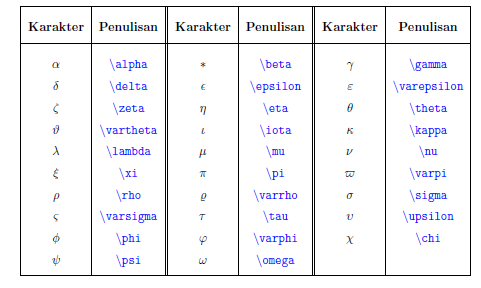
\includegraphics[width=10 cm]{img/10.png}
\end{figure}
\begin{raggedleft}Tabel 5.2 berikut ini memuat huruf kapital Yunani dan cara penulisannya dalam  LATEX\end{raggedleft}\\[0.5 cm]
\begin{figure}[h!]
\centering
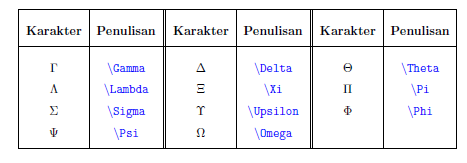
\includegraphics[width=10 cm]{img/11.png}
\end{figure}
\section{Tanda Kurung Dalam Matematika}
Penulisan tanda kurung dalam notasi matematis tidak bisa2 menggunakan tanda kurung biasa. Cara penulisan yang akan mengeluarkan notasi matematika yang baik adalah sebagai berikut :\\[0.5 cm]
\begin{tabular}{lll}
\textbackslash right delimiter& :& untuk menghasilkan tanda kurung sebelah kanan\\
\textbackslash left delimiter& : &untuk menghasilkan tanda kurung sebelah kiri\\
\end{tabular}\\[0.5 cm]
Delimiter sendiri adalah tanda kurung biasa yang penulisannya tentunya sesuai standar perintah LATEX . Beberapa delimiter yang biasa digunakan dalam notasi matematika ditunjukkan dalam Tabel 5.3 :\\[0.5 cm]
\begin{figure}[h!]
\centering
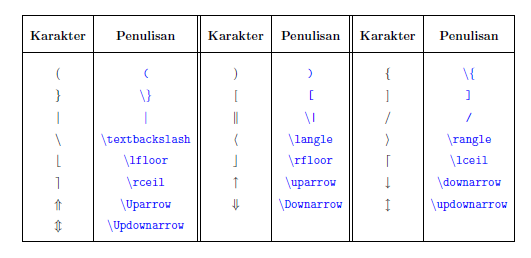
\includegraphics[width=10 cm]{img/12.png}
\end{figure}\\[0.5 cm]
\section{Penulisan Akar}
Format perintah untuk menghasilkan akar matematik adalah sebagai berikut:\\[0.5 cm]
\begin{tabular}{|p{13.5 cm}|}
\hline
\textbackslash sqrt[pangkat]\{bilangan yang diakar\}\\
\hline
\end{tabular}\\[0.5 cm]
  Contoh pemakaiannya adalah sebagai berikut :\\[0.5 cm]
\begin{tabular}{|p{13.5 cm}|}
\hline
\textbackslash begin\{displaymath\}\\
   \textbackslash sqrt[2]\{a+b\}\\
\textbackslash end\{displaymath\}\\
\hline
\end{tabular}\\[0.5 cm]
 Perintah di atas akan menghasilkan notasi seperti berikut :\\[0.5 cm]
\begin{displaymath}
\sqrt[2]{a+b}
\end{displaymath}
\section{Penulisan Pecahan}
Format perintah untuk menghasilkan notasi pecahan adalah sebagai berikut :\\[0.5 cm]
\begin{tabular}{|p{13.5 cm}|}
\hline
\textbackslash frac\{numerator\}\{denominator\}\\
\hline
\end{tabular}\\[0.5 cm]
Contoh pemakaiannya adalah sebagai berikut :\\[0.5 cm]
\begin{tabular}{|p{13.5 cm}|}
\hline
\textbackslash begin\{displaymath\}\\
   \textbackslash frac\{12x\}\{x+1\}\\
\textbackslash end\{displaymath\}\\
\hline
\end{tabular}\\[0.5 cm]
Perintah di atas akan menghasilkan notasi seperti berikut :\\[0.5 cm]
\begin{displaymath}
\frac{12x}{x+1}
\end{displaymath}
\section{Penulisan Array \& Matriks}
Sebuah array/matriks dituliskan dalam environment tabular sama seperti cara pembuatan
tabel. Perintah untuk menghasilkan sebuah array atau matriks adalah seperti berikut :\\[0.5 cm]
\begin{tabular}{|p{13.5 cm}|}
\hline
\textbackslash begin\{displaymath\}\\
   \textbackslash left (\\
\textbackslash begin\{array\}\{rrr\}\\
0 \& 45 \& 23 \\
34\& -93 \& 68 \textbackslash end\{array\}\\
\textbackslash right )\\

\textbackslash end\{displaymath\}\\
\hline
\end{tabular}\\[0.5 cm]
Contoh perintah di atas akan menghasilkan matriks seperti berikut ini :\\[0.5 cm]
\begin{displaymath}
\left (
\begin{array}{rrr}
0 & 45 & 23 \\
34& -93 & 68 \end{array}
\right )
\end{displaymath}\\[0.5 cm]
Beberapa hal yang perlu diketahui dari format perintah tersebut di atas :
\begin{itemize}
\item	Sama seperti cara penulisan tabel, huruf r di bagian belakang \textbackslash begin\\\{array\}\{rrr\} fungsinya adalah menentukan posisi dari masing-masing komponen matriks tersebut. Dalam hal ini masing-masing komponen matriks dibuat menjadi rata kanan.
\item	Tanda kurung yang digunakan adalah berupa tanda kurung kurawal. Bagian kurung buka dan kurung tutup didefinisikan masing-masing.
\end{itemize}
\section{Penulisan  Vektors}
Penulisan vektor dalam LATEX menggunakan perintah seperti berikut ini :\\[0.5 cm]
\begin{tabular}{|p{13.5 cm}|}
\hline
\textbackslash begin\{displaymath\}\\
\textbackslash vec\{variabel\}

\textbackslash end\{displaymath\}\\
\hline
\end{tabular}\\[0.5 cm]
Misalnya :\\[0.5 cm]
\begin{tabular}{|p{13.5 cm}|}
\hline
\textbackslash begin\{displaymath\}\\
\textbackslash vec\{x\}

\textbackslash end\{displaymath\}\\
\hline
\end{tabular}\\[0.5 cm]
akan menghasilkan vector seperti :\\[0.5 cm]
\begin{displaymath}
\vec{x}
\end{displaymath}
\section{Penulisan Fungsi Matematika}
Ada cukup banyak fungsi matematika yang memiliki perintah khusus untuk menuliskannya
dalam dokumen LATEX seperti misalnya sinus, cosinus, dll. Berikut adalah  tabel yang
menampilkan beberapa fungsi tersebut :\\[0.5 cm]
\begin{figure}[h!]
\centering
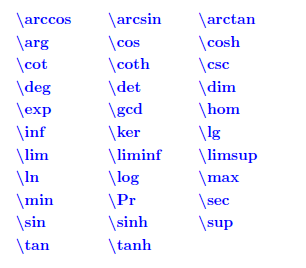
\includegraphics[width=7 cm]{img/13.png}
\end{figure}
\newpage
\section{Simbol-Simbol Matematika}
\begin{raggedleft}Untuk dapat menggunakan berbagai simbol matematika, kita harus mendeklarasikan penggunaan paket amsmath pada bagian preamble. Berikut menunjukkan simbol-simbol matematika serta perintah penulisannya dalam LATEX .\end{raggedleft}\\[0.5 cm]
\begin{figure}[h!]
\centering
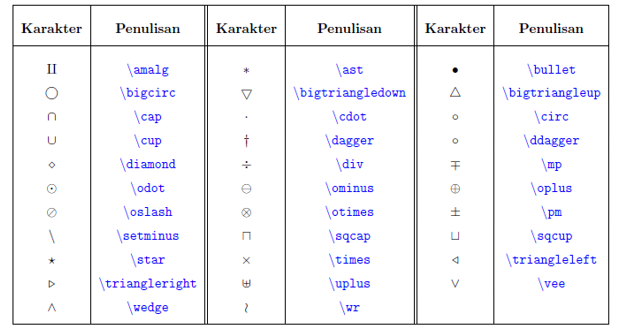
\includegraphics[width=10 cm]{img/14.png}
\end{figure}

\begin{figure}[h!]
\centering
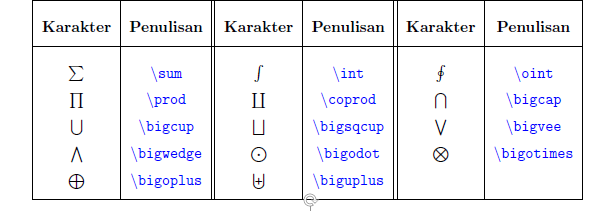
\includegraphics[width=10 cm]{img/15.png}
\end{figure}

\begin{figure}[h!]
\centering
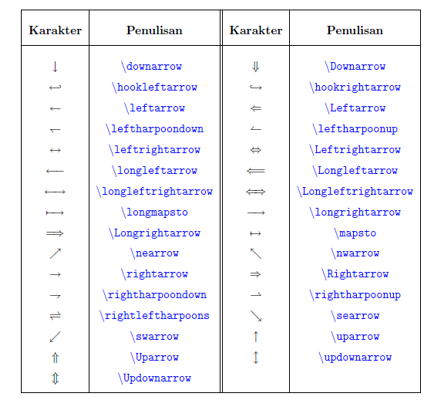
\includegraphics[width=10 cm]{img/16.png}
\end{figure}

\begin{figure}[h!]
\centering
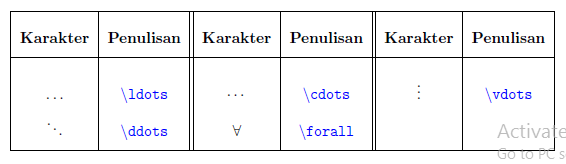
\includegraphics[width=10 cm]{img/17.png}
\end{figure}
\newpage
\section{Membuat halaman landscape dan portrait}
Dalam latex, dapat membuat dan meletakkan dokumen dengan landscape maupun  portrait sebagai contoh:\\[0.5 cm]
\begin{tabular}{|p{13.5 cm}|}
\hline
\textbackslash documentclass[12pt,a4paper]\{report\}\\
\textbackslash usepackage\{lscape\}\\
\textbackslash begin\{document\}\\
\textbackslash  pagenumbering\{arabic\}\\
\textbackslash chapter\{Title 1\}\\
\textbackslash  begin\{landscape\}\\
\textbackslash centering\\
Text here.\\
\textbackslash end\{landscape\}\\
\textbackslash  chapter\{Title 2\}\\
\textbackslash  end\{document\}\\
\hline
\end{tabular}\\[0.5 cm]
hasil output-nya:\\
\begin{enumerate}
\item halaman pertama
\begin{figure}[h!]
\centering
\fbox{
\includegraphics[width=10 cm]{img/28.png}}
\end{figure}
\item halaman kedua
\begin{figure}[h!]
\centering
\fbox{
\includegraphics[width=10 cm]{img/29.png}}
\end{figure}
\newpage
\item halaman ketiga
\begin{figure}[h!]
\centering
\fbox{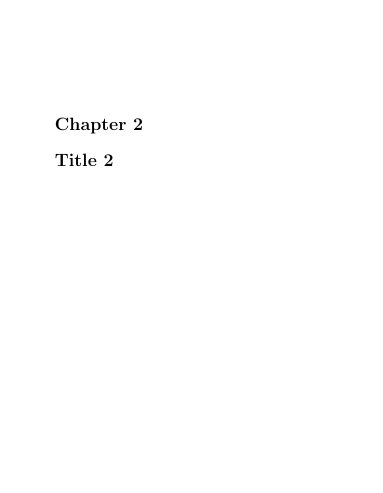
\includegraphics[width=10 cm]{img/30.png}}
\end{figure}
\end{enumerate}
\section{memberikan warna dalam tabel}
Dalam latex, kita dapat memberikan waarna pada setiap baris maupun kolom dalam tabel sebagai contoh sebagai berikut:\\[0.5cm]
\begin{enumerate}
\newpage
\item perwarnaan pada baris tabel\\
\begin{tabular}{|p{12.5 cm}|}
\hline
\textbackslash documentclass[11pt,a4paper]\{article\}\\
\textbackslash usepackage[T1]\{fontenc\}\\
\textbackslash usepackage[latin1]\{inputenc\}\\
\textbackslash usepackage[table]\{xcolor\}\\    % loads also »colortbl«

\textbackslash begin\{document\}\\
  \textbackslash rowcolors\{2\}\{gray!25\}\{white\}\\
  \textbackslash begin\{tabular\}\{cc\}\\
    \textbackslash rowcolor\{gray!50\}\\
    Table head \& Table head  \textbackslash \textbackslash \\
    Some values \& Some values\textbackslash \textbackslash  \\
    Some values \& Some values \textbackslash \textbackslash \\
    Some values \& Some values \textbackslash \textbackslash  \\
    Some values \& Some values\\
  \textbackslash  end\{tabular\}\\
\textbackslash end\{document\}\\
\hline
\end{tabular}\\[0.5 cm]
 hasil outputnya:\\
\begin{figure}[h!]
\centering
\fbox{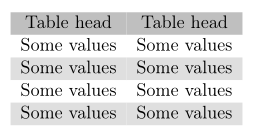
\includegraphics[width=10 cm]{img/31.png}}
\end{figure}
\newpage
\item perwarnaan pada kolom tabel\\
\begin{tabular}{|p{12.5 cm}|}
\hline
 \textbackslash newcolumntype\{g\}\{\textgreater \{ \textbackslash columncolor\{red\}\}c\}\\
 \textbackslash begin\{table\}[ht]\\
 \textbackslash centering\\
 \textbackslash begin\{tabular\}\{c \textbar g \textbar c \textbar g\textbar c \textbar g\textbar c\textbar g\}\\
 \textbackslash hline\\
\&col1 \&col2 \&col3 \&col4 \& col5 \&col6 \&col7\textbackslash\textbackslash\\
 \textbackslash hline \\
row1\& 1 \&2 \& 3  \& 4 \& 5 \& 6 \&7 \textbackslash \textbackslash\\
row2\& 2 \& 3 \& 5 \& 6 \& 7 \& 1 \& 1 \textbackslash\textbackslash\\
row3\& 3 \& 4 \& 6 \& 7 \& 1 \& 2 \& 2 \textbackslash\textbackslash \\
row4\& 4 \& 5 \& 7\& 1 \& 2 \& 3 \& 3  \textbackslash\textbackslash\\
row5\& 5 \& 6 \& 1\& 2 \& 3 \& 4 \& 4  \textbackslash\textbackslash\\
row6\& 6 \& 7 \& 2 \& 3 \& 4 \& 5 \& 5  \textbackslash\textbackslash\\
\textbackslash hline\\
  \textbackslash  end\{tabular\}\\
  \textbackslash  end\{table\}\\
\hline
\end{tabular}\\[0.5 cm]
 hasil outputnya:\\
\newcolumntype{g}{>{\columncolor{yellow}}c}
\begin{tabular}{c|g|c|g|c|g|c|g}
\hline
       &col1 &col2 &col3 &col4 & col5 &col6 &col7\\
\hline
row1& 1 &2 & 3  & 4 & 5 & 6 &7\\
row2& 2 & 3 & 5 & 6 & 7 & 1 & 1 \\
row3& 3 & 4 & 6 & 7 & 1 & 2 & 2 \\
row4& 4 & 5 & 7& 1 & 2 & 3 & 3 \\
row5& 5 & 6 & 1 & 2 & 3 & 4 & 4 \\
row6& 6 & 7 & 2 & 3 & 4 & 5 & 5 \\
\hline
\end{tabular}
\end{enumerate}
\section{mengubah {\itshape font size} dalam tabel}
Dalam tabel kita dapat mengubah {\itshape font size} yang sesuai yang kita inginkan. Berikut contoh {\itshape source code} yang digunakan: \\[0.5 cm]
\begin{tabular}{|p{13.5 cm}|}
\hline
    \textbackslash fontsize\{10pt\}\{20pt\}\\
      \textbackslash selectfont\\

    ...table...\\

      \textbackslash fontsize\{11pt\}\{21pt\}\\
      \textbackslash selectfont\\
\hline
\end{tabular}
\section{ mengatur {\itshape margin}}
Dalam membuat dokumen, kita dapat mengatur {\itshape margin} berikut contoh kode yang digunakan:\\[0.5 cm]
\begin{tabular}{|p{13.5 cm}|}
\hline
\textbackslash usepackage[left=2cm, right=5cm, top=2cm]\{geometry\}\\
\hline
\end{tabular}
\section{Menambahkan nama pada daftar isi , daftar tabel dan daftar gambar}
\begin{enumerate}
\item Memberikan nama BAB  di tiap {\itshape chapter} dalam daftar isi.\\
\begin{tabular}{|p{12.5 cm}|}
\hline
\textbackslash renewcommand\{\textbackslash cftchappresnum\}\{BAB  \} \\
\textbackslash AtBeginDocument\{\textbackslash addtolength\textbackslash cftchapnumwidth\{\textbackslash widthof\{\textbackslash bfseries Chapter\}\}\} \\
\hline
\end{tabular}
\item  Memberikan nama Tabel di  dalam daftar tabel.\\
\begin{tabular}{|p{12.5 cm}|}
\hline
\{ \\
\textbackslash let\textbackslash oldnumberline\textbackslash numberline \\
\textbackslash renewcommand\{\textbackslash numberline\}\{\textbackslash tablename~~\textbackslash oldnumberline\} \\
\textbackslash listoftables\\
\} \\
\hline
\end{tabular}
\item  Memberikan nama Gambar di dalam daftar gambar.\\
\begin{tabular}{|p{12.5 cm}|}
\hline
\{ \\
\textbackslash let\textbackslash oldnumberline\textbackslash numberline\\
\textbackslash renewcommand\{\textbackslash numberline\}\{\textbackslash figurename~~\textbackslash oldnumberline\} \\
\textbackslash listoffigures\\
\} \\
\hline
\end{tabular}
\end{enumerate}
	
	\setcounter{page}{1}
	\chapter{PENDAHULUAN}
\section{Latar Belakang}
Aplikasi Enterprise Resource Planning(ERP) merupakan perangkat lunak yang digunakan pada perusahaan untuk menjalankan bisnisnya dimana perusahaan dapat mengotomatisasi dan mengintegrasi sebagian besar proses bisnisnya dengan ini perusahaan bisa menghasilkan serta mengakses informasi secara langsung [1]. Selain itu diharapkan juga aplikasi memiliki skalabilitas terhadap operasi bisnis, yang diperlukan dalam jangka panjang, misalkan ketika perusahaan tumbuh dari waktu ke waktu, serta dalam waktu singkat, misalnya pada saat volume transaksi tinggi seperti belanja Natal \cite{1}.

Dalam membangun aplikasi ERP umumnya dibangun dengan beberapa arsitektur seperti \textit{ two-tier, three-tier/n-tier,} dan \textit{service oriented architecture(SOA)} dimana arsitektur ini disebarkan secara monolit. Saat ini arsitektur yang umum digunakan yaitu SOA karena dapat membantu perancangan ERP menjadi lebih terukur, andal dan fleksibel dengan memecah fungsionalitas menjadi bagian kecil yang dinamakan service \cite{1}.

SOA memiliki keuntungan dalam melakukan pemeriksaan status aplikasi, melakukan perutean untuk service backend, meskipun demikian ditemukan bahwa SOA bisa menjadi rumit dan menyebabkan terjadinya bottleneck. Arsitektur Microservice(MSA) dapat menangani kekurangan ini dengan terisolasi, independen dan mudah didistribusikan sehingga memudahkan skalabilitas. Keuntungan terbesarnya yaitu aplikasi bisa dibangun dengan berbagai pilihan teknologi dan memungkinkannya untuk digunakan secara independen satu sama lain. Ini sangat menyederhanakan siklus pengembangan, pengujian, pembuatan, dan penerapan aplikasi karena perubahan terbatas pada satu service daripada seluruh aplikasi \cite{3}.

Hal ini dibuktikan juga dengan penelitian sebelumnya yang melakukan uji performa berupa uji beban dari setiap arsitektur. Dimana MSA memiliki throughput yang lebih tinggi pada 1500 pengguna dengan nilai rata-rata 1,1 dibandingkan dengan arsitektur SOA sebesar 0,7 dan monolith sebesar 0,6. Selain itu pada response time MSA lebih cepat 5 detik yaitu sebesar 33 detik dibandingkan dengan monolith sebesar 38 detik dan SOA sebesar 43 detik.

Pada pengukuran jumlah kode response 200(Berhasil), MSA memiliki jumlah response tertinggi di kode berhasil dengan memiliki jumlah response terkecil di kode 302(Pengalihan), 304(Cache) ,408(Waktu Habis), 500(Kesalahan Internal Server) dan tidak memiliki jumlah response di kode 404(Tidak ditemukan). Dimana pada aspek pemeliharaan aplikasi, MSA lebih unggul daripada SOA dan monolit unggul daripada SOA \cite{4}.

Naman manfaat ini hanya dapat dimanfaatkan jika service didekomposisi dengan cara yang paling optimal dengan mempertimbangkan gambaran besar dari seluruh cakupan aplikasi. Jika tidak, desain ini mungkin terbukti kontraproduktif dan menyebabkan latensi, kompleksitas, dan inefisiensi Hal ini diperlukan untuk memisahkan aplikasi menjadi bagian-bagian yang sesuai secara fungsional dan memperoleh service kohesif tinggi dan service yang digabungkan secara longgar diharapkan sebagai hasil dari dekomposisi \cite{3}.

Dalam melakukan dekomposisi bisa dilakukan dengan konsep Domain Driven Design(DDD), Functional, Dataflow, dan Dependency Capturing dengan Clustering. Pada hasil evaluasi DDD menunjukkan aplikasi berhasil didekomposisi ke microservice. Dengan pendekatan Functional hasil evaluasi menunjukkan bahwa identifikasi microservice dapat dilakukan lebih cepat. Di pendekatan dataflow ini menunjukkan dekomposisi bisa ditentukan dari pertimbangan coupling dan kohesi. Identifikasi microservice dengan menganalisis ketergantungan proses bisnis dari control, dengan data dan control, data, dan semantic models. Kemudian untuk metode Clustering untuk mengidentifikasi microservice, metode clustering yang digunakan yaitu Hierarchical Clustering. Hasil dari validasi pendekatan ini menunjukkan bahwa pendekatan ini mencapai hasil yang lebih baik daripada pendekatan yang ada dalam hal identifikasi microservice \cite{5}.

Pada penelitian ini akan melakukan dekomposisi aplikasi ERP yang disebarkan secara monolit menjadi arsitektur microservice dengan pendekatan menganalisis graph yang dihasilkan dari source code kemudian dilakukan pengelompokan melalui Hierarchical Clustering. Hasil dari pengelompokan akan diimplementasikan dan dilakukan uji beban sehingga mengetahui nilai latensi, jumlah throughput, dan penggunaan sumber daya komputasi. Dengan ini diharapkan bisa menyelesaikan permasalahan yang terjadi di aplikasi ERP seperti kustomisasi dan skalabilitas.\\

\section{Rumusan Masalah}
Berikut adalah rumusan masalah yang dibuat berdasarkan latar belakang diatas.
\begin{enumerate}[nolistsep,leftmargin=0.5cm]
  \item Bagaimana nilai kohesi dan kopel yang dihasilkan dari dekomposisi melalui pendekatan Hierarchical Clustering?
  \item Bagaimana performa aplikasi ERP antara arsitektur monolit dan arsitektur microservice dalam kondisi beban yang tinggi?
  \item Berapa besar penggunaan sumber daya aplikasi ERP yang digunakan pada arsitektur monolit dibandingkan arsitektur microservice?\\
\end{enumerate}

\section{Tujuan Penelitian}
Berdasarkan rumusan masalah di atas, maka tujuan tujuan penelitian ini adalah.
\begin{enumerate}[nolistsep,leftmargin=0.5cm]
  \item Menerapkan dekomposisi aplikasi ERP monolit ke microservice dengan pendekatan Hierarchical Clustering.
  \item Mencari kelompok service yang memiliki nilai kopel rendah dan nilai kohesi tinggi.
  \item Membandingkan performa dan sumber daya aplikasi ERP dengan bentuk pengelompokan yang berbeda di arsitektur microservice. \\
\end{enumerate}

\section{Batasan Masalah}
Agar penelitian ini menjadi lebih terarah, maka penulis membatasi masalah yang akan dibahas sebagai berikut.
\begin{enumerate}[nolistsep,leftmargin=0.5cm]
  \item Penyebaran aplikasi dilakukan dengan framework docker.
  \item Aplikasi yang digunakan adalah aplikasi yang sudah dibangun sebelumnya dan disebarkan dengan arsitektur monolit.
  \item Perubahan arsitektur tidak menambah atau mengurangi fungsionalitas dari aplikasi.\\
  \item Hanya module utama pada ERP yang akan dilakukan dekomposisi
\end{enumerate}

\section{Konstribusi Penelitian}
Kontribusi yang diberikan pada penelitian ini adalah sebagai berikut.
\begin{enumerate}[nolistsep,leftmargin=0.5cm]
  \item Memberikan langkah dalam melakukan dekomposisi aplikasi monolit ke microservice dengan Hierarchical Clustering.
  \item Mengetahui pengaruh dari performa aplikasi yang sudah dilakukan dekomposisi dengan uji beban pada aplikasi.
  \item Membuat aplikasi microservice yang memiliki nilai kohesi tinggi dan nilai kopel rendah.\\
\end{enumerate}

\section{Metodologi Penelitian}
Tahapan-tahapan yang akan dilakukan dalam pelaksanaan penelitian ini adalah sebagai berikut.
\begin{enumerate}[nolistsep,leftmargin=0.5cm]
  \item Penelitian Pustaka \\
  Penelitian ini dimulai dengan studi kepustakaan yaitu mengumpulkan referensi baik dari buku, paper, jurnal, atau artikel daring mengenai arsitektur microservice, permasalahan pada aplikasi ERP dan dekomposisi monolit ke microservice.
  \item Analisis
  Dilakukan analisis permasalahan yang ada, batasan-batasan yang ditentukan, dan  kebutuhan-kebutuhan yang diperlukan untuk menyelesaikan permasalahan yang ditemukan.
  \item Perancangan \\
  Pada tahap ini dilakukan perancangan untuk melakukan dekomposisi dari aplikasi arsitektur monolit ke arsitektur microservice dengan dengan pendekatan Hierarchical Clustering.
  \item Implementasi \\
  Pada tahap ini mengimplementasikan hasil perancangan dekomposisi ke aplikasi microservice pada aplikasi yang dibuat dengan arsitektur monolit.
  \item Pengujian \\
  Pada tahap ini  dilakukan pengujian pada aplikasi yang sudah di dekomposisi. Pengujian melalui uji beban akan dilakukan dengan perbandingan antara aplikasi monolit dan aplikasi microservice.\\ 
\end{enumerate}

\section{Sistematika Pembahasan}
\textbf{BAB 1: PENDAHULUAN} \\
Pendahuluan yang berisi latar belakang, rumusan masalah, tujuan penelitian, batasan masalah, kontribusi penelitian, serta metode penelitian.

\textbf{BAB 2: LANDASAN TEORI}\\
Landasan Teori yang berisi penjelasan dasar teori yang mendukung penelitian ini, seperti arsitektur monolit, arsitektur microservice, hierarchical clustering, dan dekomposisi.

\textbf{BAB 3: ANALISIS DAN PERANCANGAN}\\
Analisis dan Perancangan yang berisi tahapan penerapan dekomposisi aplikasi monolit ke microservice dengan hierarchical clustering dan penyebaran aplikasi melalui kontainer.

\textbf{BAB 4: IMPLEMENTASI DAN PENGUJIAN}\\
Implementasi dan Pengujian yang berisi pembangunan aplikasi dan pengujian dengan mensimulasikan dan mengevaluasi aplikasi yang telah didekomposisi.

\textbf{BAB 5: KESIMPULAN DAN SARAN}\\
Penutup yang berisi kesimpulan dari penelitian dan saran untuk penelitian lebih lanjut di masa mendatang.
	
	\setcounter{page}{1}
	%-----------------------------------------------------------------------------%
\chapter{LANDASAN TEORI}
%-----------------------------------------------------------------------------%
\vspace{4.5pt}
Pada bab ini menjelaskan beberapa teori dan jurnal yang berhubungan dengan permasalahan penelitian yang digunakan pada proses penelitian.
\section{Tinjauan Pustaka}
Pembahasan mengenai teori-teori tersebut dijelaskan sebagai berikut.
\subsection{Monolit}
Monolit yaitu suatu cara untuk melakukan penyebaran. Ketika semua fungsi dalam sistem harus disebarkan secara bersama-sama, maka itu merupakan sebuah monolit \cite{6}. Monolit merupakan sebuah aplikasi perangkat lunak dimana setiap modulnya tidak bisa dieksekusi secara independen. Hal ini membuat monolit sulit digunakan pada sistem terdistribusi tanpa bantuan penggunaan \textit{frameworks} atau solusi \textit{ad hoc} seperti Objek Jaringan, \textit{RMI} atau \textit{CORBA} \cite{16}.

Penggunaan pada bahasa pemrograman seperti \textit{Java},\textit{C/C++}, dan \textit{Python} pada pengembangan aplikasi di sisi \textit{server}, memiliki kemampuan dalam melakukan abstraksi untuk memecah kompleksitas program menjadi berupa modul. Namun, bahasa pemrograman ini dirancang untuk membuat \textit{artefacts} monolit. Dimana abstraksi ini tergantung pada penggunaan berbagi sumber data pada komputer yang sama (memori, database, file) \cite{16}.


Terdapat 3 jenis monolit \cite{6}:
\begin{enumerate}[leftmargin=1.3cm]
\item \textit{Single Process Monolith}\\
Dimana sebuah kode disebarkan dengan satu proses. Setiap kode bisa berada di banyak \textit{instances} serta tempat penyimpanan dan mendapatkan data disimpan pada suatu database yang sama. Variasi lainnya yaitu modular monolit dimana setiap kode bisa bekerja secara independen tetapi perlu dijadikan satu kesatuan ketika ingin dilakukan \textit{deployment}.
\item \textit{Distributed Monolith}\\
Monolit terdistribusi adalah sistem yang terdiri dari beberapa layanan, tetapi untuk apa pun alasannya seluruh sistem harus disebarkan bersama-sama. Sebuah monolit terdistribusi bisa memiliki kesamaan dengan \textit{service-oriented architecture (SOA)}.

Monolit terdistribusi biasanya muncul  di kondisi dimana tidak cukup fokus pada konsep \textit{information hiding} dan kohesi dari fungsi bisnis. Akibatnya terbentuklah arsitektur yang memiliki kopel yang tinggi, dimana bisa perubahan menyebabkan kerusakan pada bagian sistem lain.
\item \textit{Sistem Black-Box Pihak Ketiga}\\
Aplikasi pihak ketiga merupakan sebuah monolit, misalkan sistem penggajian, sistem CRM, dan sistem SDM. Faktor umum yang terjadi yaitu aplikasi ini dibuat dan dikelola oleh orang lain dimana pengembang belum tentu memiliki kemampuan untuk mengubah kode seperti \textit{Software-as-a-Service(SaaS)}.
\end{enumerate}

Keuntungan dari Monolit \cite{6,8}:
\begin{enumerate}[leftmargin=1.3cm]
\item Sederhana dalam melakukan pengembangan karena \textit{Integrated Development Environment (IDE)} dan peralatan pengembang berfokus pada membuat satu aplikasi
\item Mudah untuk melakukan perubahan secara radikal di aplikasi. Perubahan ini bisa dari kode hingga skema database serta proses \textit{deployment}.
\item Pengujian dilakukan pada satu aplikasi, pengembang dapat membuat pengujian dari awal hingga akhir dengan lebih mudah dan terintegrasi
\item Deployment dilakukan pada satu aplikasi, pengembang hanya menyalin aplikasi dari komputer ke komputer yang lain. Dengan ini aplikasi relatif mudah dilakukan konfigurasi dan mudah diperbanyak jumlah aplikasi.
\end{enumerate}

Tantangan dari monolit \cite{6,8}:
\begin{enumerate}[leftmargin=1.3cm]
	\item Sulit dikembangkan secara berkelanjutan, karena semakin banyak orang yang bekerja pada aplikasi yang sama. Akibatnya setiap pengembang memiliki kepentingan masing-masing dalam mengelola kode yang sama dan membuat pengambilan keputusan sulit serta tidak fleksibel
	\item Memiliki reliabilitas yang rendah, karena kesalahan pada salah satu module aplikasi bisa menyebabkan kegagalan secara keseluruhan aplikasi. Akibatnya aplikasi tidak dapat digunakan oleh pengguna dan harus dilakukan deployment kembali.
	\item Tidak mudah untuk melakukan skalabilitas,setiap modul aplikasi memiliki kebutuhan sumber daya yang berbeda seperti ada module penyediaan data yang membutuhkan banyak memori sedangkan modul pemprosesan gambar membutuhkan banyak CPU, karena module ini berada pada aplikasi yang sama akibatnya pengembang harus melakukan pengorbanan pada salah satu sisi sumber daya.
	\item Terkunci pada teknologi jadul, pengembang terkunci pada teknologi awal yang digunakan untuk membangun aplikasi. Pengembang juga kesulitan ketika ingin mengadopsi teknologi baru pada aplikasi karena sangat berisiko dan sangat mahal untuk menulis kembali seluruh aplikasi antar teknologi.\\
\end{enumerate}	

\subsection{\textit{Microservice}}
\textit{Microservice} adalah beberapa \textit{service} yang bisa di deploy secara independen yang dimodelkan berdasarkan bisnis domain. \textit{Service} ini berkomunikasi satu sama lain melalui jaringan komputer dan bisa dibangun dengan berbagai macam teknologi. \textit{Microservice} adalah salah tipe dari \textit{service oriented architecture (SOA)} meskipun ada perbedaan dalam membuat batasan antara \textit{service} dan \textit{deployment} secara independen \cite{8}.

\textit{Service} adalah komponen perangkat lunak yang memiliki kegunaannya secara khusus dimana komponen ini bisa berdiri sendiri dan secara independen dilakukan proses deployment. Service memiliki \textit{API (Application Programming Interface)} yang memberikan akses kepada \textit{client} untuk melakukan operasi. Terdapat 2 tipe operasi yaitu perintah dan kueri.
\textit{API} terdiri dari perintah, kueri dan \textit{event}. Perintah dapat berupa \textit{buatPesanan()} yang melakukan aksi dan memperbarui data. Kueri dapat berupa \textit{cariPesananBerdasarkanID()} yang digunakan untuk mengambil data. \textit{Service} juga dapat membuat suatu \textit{event} seperti \textit{PesananSudahDibuat} dimana \textit{event} ini akan dikonsumsi oleh \textit{client}-nya / \textit{subscriber} \cite{8}.

\textit{Service API} akan mengenkapsulasi internal implementasinya, sehingga pengembang aplikasi tidak bisa menuliskan kode yang melewati \textit{API}. Akibatnya arsitektur \textit{microservice} dapat mewajibkan modularitas di aplikasi.  Setiap \textit{service} di arsitektur \textit{microservice} memiliki masing-masing arsitektur sendiri dan dimungkinkan dengan teknologi yang berbeda. Tetapi kebanyakan \textit{service} memiliki arsitektur heksagonal. Dimana \textit{API} akan diimplementasi melalui adapter yang berinteraksi dengan logika bisnis \cite{7}

Ciri Khusus \textit{Microservice} \cite{6,7,8}:	
\begin{enumerate}[leftmargin=1.3cm]
	\item Kecil dan berfokus pada satu hal dengan baik\\
	\textit{Service} yang dibuat memiliki \textit{encapsulation} dengan pembuatan \textit{service} dimodelkan di sekitar Domain Bisnis, tujuannya agar ketika terjadi perubahan antar \textit{service} bisa dilakukan dengan lebih mudah dan tidak berdampak pada \textit{service} lain. Oleh karena itu \textit{service} yang dibuat seminimal mungkin untuk tidak berhubungan dengan \textit{service} lain. 
	\item Otonomi / Bisa berdiri sendiri\\
	\textit{Microservice} memiliki \textit{service} yang terisolasi dimana bisa memiliki sistem operasi hingga komputer yang berbeda. Dengan ini sistem terdistribusi lebih sederhana dan nilai kopel yang rendah. Semua komunikasi antar service dilakukan melalui jaringan sehingga \textit{service} harus memiliki kemampuan di\textit{deploy} sendiri tanpa harus mempengaruhi \textit{service} lain.
	\item Data yang dikelola masing-masing \textit{service}\\
	\textit{Service} yang membutuhkan data diluar domainnya harus berkomunikasi melalui \textit{API(application programming interface)}, dengan ini setiap \textit{service} memiliki tanggung jawab terhadap datanya masing-masing sehingga data tersebut hanya bisa diubah oleh \textit{service} itu sendiri. Setiap \textit{service} memiliki data yang pribadi dan data yang bisa dibagikan kepada \textit{service} lain
\end{enumerate}	

Keuntungan dari \textit{Microservice}  \cite{6,7,8}:
\begin{enumerate}[leftmargin=1.3cm]
	\item Memudahkan pengembangan aplikasi kompleks dan flexibel\\
	\textit{Service} berukuran kecil sehingga mudah dikelola, perubahan pada satu \textit{service} bisa diterapkan secara independen dari service lainnya. Bila terjadi kegagalan di satu \textit{service} tidak berdampak besar pada \textit{service} lainnya karena \textit{service} masing-masing terisolasi selain itu proses pemulihan bisa dilakukan dengan mudah dan cepat.
	\item Bisa dilakukan skaling secara independen\\ 
	Setiap \textit{service} memiliki fungsi yang berfokus pada satu hal,  dimana setiap \textit{service} bisa memiliki kebutuhan sumber daya berbeda. Penggunaan sumber daya ini bisa dikelola dengan mudah dan cepat karena setiap service dapat di\textit{deploy} dengan jumlah \textit{service} yang berbeda.
	\item Mudah melakukan percobaan dan penggunaan teknologi baru\\
	Arsitektur \textit{microservice} mengeliminasi komitmen penggunaan secara lama pada suatu teknologi. Dengan ini pengembang dapat memilih berbagai teknologi dalam membangun \textit{service} serta \textit{service} yang kecil dan berfokus lebih mudah untuk dilakukan migrasi antara teknologi yang berbeda. 
\end{enumerate}	

Tantangan dari \textit{Microservice}  \cite{6,7,8}:
\begin{enumerate}[leftmargin=1.3cm]
	\item Menemukan \textit{service} yang tepat itu sulit\\
	Salah satu tantang terbesar dari membuat \textit{microservice} yaitu tidak adanya cara yang pasti bagaimana untuk melakukan dekomposisi dengan baik. Dimana \textit{service} yang didekomposisi dengan tepat tidak mudah ditemukan dan bila dilakukan dengan tidak benar dapat sebaliknya membuat \textit{distributed monolith}. 
	\item Memiliki kompleksitas karena merupakan suatu terdistribusi\\
	Setiap \textit{service} untuk berkomunikasi antar \textit{service} memiliki tantangan masing-masing seperti latensi, konsistensi data, dan kondisi ketika beberapa \textit{service} mengalami kegagalan. \textit{Microservice} juga meningkatkan kompleksitas operasional oleh karena itu untuk melakukan \textit{deployment} sebaiknya menggunakan proses otomatisasi.
	\item \textit{Deployment} yang melibatkan beberapa service\\
	Untuk melakukan \textit{deployment} ini dibutuhkan koordinasi antara tim pengembang \textit{servic} ketika menambahkan atau mengubah fitur yang berdampak pada beberapa \textit{service} maka dari itu harus dibuat perencanaan \textit{deployment} berdasarkan ketergantungan antar \textit{service}.
\end{enumerate}	

Pola \textit{Microservice}  \cite{8}:
\begin{center}
	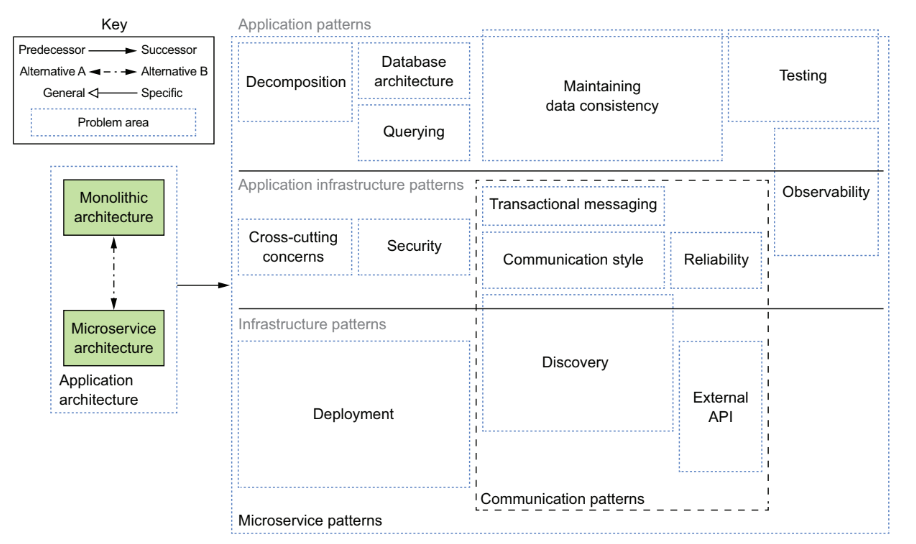
\includegraphics[width=12cm]{img/PolaMicroservice.png}
	\captionof{figure}{
	Pola dalam menyelesaikan masalah di arsitektur \textit{Microservice} \cite{8} }
	\label{fig:msa}
\end{center}
\begin{enumerate}[leftmargin=1.3cm]
	\item \textit{Application patterns}
	Permasalahan yang harus diselesaikan oleh pengembang aplikasi
	- Proses kueri
	- Dekomposisi aplikasi menjadi service
	- Menjaga data konsistensi dan implementasi proses transaksi
	- Mengotomatiskan proses pengujian  service ...
	\item \textit{Application infrastructure} 
	Permasalah infrastruktur yang memiliki pengaruh pada proses pengembangan aplikasi
	- Pola komunikasi
	- Pola mengatasi permasalahan antar service ...
	\item \textit{Infrastructure patterns} 
	Permasalahan infrastruktur yang muncul diluar dari pengembangan aplikasi
	- Pola Komunikasi
	- Pola Service Deployment
	- Pola observability untuk mengetahui bagaimana aplikasi bekerja ...\\	
\end{enumerate}	

\subsection{\textit{Enterprise Resource Planning}}
\textit{Enterprise Resource Planning} (ERP) adalah suatu sistem perangkat lunak yang memungkinkan perusahaan untuk mengotomatisasikan dan mengintegrasikan proses bisnisnya dengan komputerisasi. Dengan ini setiap informasi yang diperlukan di proses bisnis dapat dibagikan dan digunakan disemua bagian perusahaan dengan alur terstruktur. Sistem ERP dapat mengeliminasi duplikasi data dan memberikan integrasi data. Sistem ERP memiliki database dimana semua transaksi bisnis dapat direkam, diproses, dipantau dan dilaporkan. Tujuannya agar proses bisnis bisa dilakukan dengan lebih cepat, murah, dan transparan \cite{1}.

Sistem ERP dapat memberikan dukungan untuk proses bisnis perusahaan melalui modul yang terpisah. Setiap modul adalah aplikasi perangkat lunak yang dibangun khusus untuk setiap operasi bisnis. Umumnya modul yang ditemukan pada ERP yaitu Modul Produksi, Modul Manajemen Rantai Pasokan, Modul Keuangan, Modul Penjualan \& Pemasaran, Modul Sumber Daya Manusia, dan modul pelengkap lainnya seperti \textit{e-commerce} \cite{1}.

Arsitektur ERP \cite{1}: 
\begin{enumerate}[leftmargin=1.3cm]
	\item \textit{The Tiered}\\
	Arsitektur \textit{tiered} umumnya dirancang dalam bentuk lapisan yang didasarkan dari model \textit{client-server} atau bisa disebut \textit{N-Tier}. Dalam arsitektur ini setiap komponen ERP disusun kedalam masing lapisan seperti lapisan \textit{user interface}, lapisan aplikasi dan lapisan \textit{database} / penyimpanan data.
	\item \textit{Web-based}\\
	Arsitektur \textit{Web-based} mengadopsi teknologi berorientasi objek web dimana pengguna yang ingin menggunakan sistem ERP bisa mengakses melalui \textit{browser} dan internet. \textit{Object-oriented technology} diimplementasi untuk mencampur data dan fungsi yang tersedia di berbagai web \textit{service}.
	\item \textit{Service Oriented}\\
	\textit{SOA(Service Oriented Architecture)} adalah sistem yang dimana terdapat fungsi  modular yang berkomunikasi melalui jaringan. Satu atau lebih \textit{service} bisa berkordinasi dalam suatu aktivitas fungsi bisnis. 
	\item \textit{Cloud}\\
	\textit{Cloud} dapat memberikan solusi bagi organisasi ketika mengadopsi sistem ERP pada kegiatan bisnisnya. Sistem ERP dengan arsitektur \textit{cloud} bisa dikategorikan sebagai tipe \textit{SaaS(Software as a Service)}. Organisasi akan membayar pihak ke tiga setiap periode berdasarkan modul yang digunakannya.\\ 
\end{enumerate}

\subsection{Analisis Kode}
Analisis Kode adalah suatu proses mengekstraksi informasi mengenai suatu program dari kode atau artifak. Proses ini bisa dilakukan secara manual yaitu dengan melihat kode program atau bahasa mesin namun kompleksitas program yang tinggi membuat proses secara manual sangat sulit dan tidak efektif. Sehingga diperlukan alat otomatisasi yang dapat membantu proses analisis kode. Alat ini dapat memberikan informasi kepada pengembang mengenai program yang dianalisis \cite{9}. 

Anatomi Analisis Kode \cite{9}:
\begin{enumerate}[leftmargin=1.3cm]
	\item Ekstraksi Data\\
	Proses ini adalah proses pertama kali dilakukan sebelum melakukan analisis kode, data yang diekstrasi berasal dari kode program. Umumnya dilakukan dengan \textit{syntatic analyzer} atau \textit{parser}. Proses \textit{Parser} ini mengkonversi urutan karakter menjadi suatu kata-kata dan mengekstraksi nilai semantik sebenarnya. Tujuannya agar memudahkan proses analisis/transformasi dan penambahan data lainnya.
	\item Representasi Informasi\\
	Proses yang merepresentasikan informasi kode menjadi bentuk yang lebih abstrak. Tujuan dari fase ini untuk membentuk beberapa bagian kode agar terhubung pada analisis secara otomatis. Representasi ini kebanyakan berupa graph seperti \textit{Abstract Syntax Trees (AST)}, \textit{Control Flow Graphs (CFG)}, dan \textit{Call Graph}.
	\item Eksplorasi Pengetahuan\\
	Setelah informasi direpresentasikan, informasi dibuat menjadi suatu kesimpulan. Kesimpulan bisa dibuat secara kuantitatif atau kualitatif, proses visualisasi penting dalam proses eksplorasi pengetahuan kode program.
\end{enumerate}

Strategi Analisis Kode \cite{9}:
\begin{enumerate}[leftmargin=1.3cm]
	\item Statik vs Dinamis\\
	Analisis secara statik menganalisis program tanpa dieksekusi untuk mendapatkan semua informasi yang kemungkinan akan dieksekusi. Sedangkan secara Dinamis, program mengumpulkan informasi yang dieksekusi dengan nilai yang diberikan. Beberapa teknik analisis menggabungkan kedua pendekatan ini.
	\item \textit{Sound vs Unsound}\\
	\textit{Sound} yaitu analisis yang bisa menjamin secara keseluruhan dan kebenaran eksekusi program. Sedangkan \textit{Unsound} tidak bisa secara keseluruhan menjaminkan kebenaran hasil analisis program. Namun dalam banyak kasus analisis \textit{Unsound} memiliki hasil yang benar selain itu memiliki kelebihan yaitu mudah diimplementasi dan efisien.
	\item \textit{Flow sensitive vs Flow insensitive}\\
	\textit{Flow sensitive} memperhatikan dan menyimpan urutan proses eksekusi sedangkan \textit{Flow insensitive} tidak memperhatikan urutan proses eksekusi sehingga tidak memiliki informasi ketergantungan pada suatu proses dan hanya dapat menyatakan proses tersebut ada.
	\item \textit{Context sensitive vs Context insensitive}\\
	\textit{Context in-sensitive} hanya menghasilkan satu hasil yang berhubungan dalam semua konteks. Sedangkan \textit{context sensitive} memiliki hasil berbeda ketika konteks berbeda. Pendekatan ini bertujuan untuk menganalisis proses pembuatan analisis umumnya tanpa adanya informasi mengenai konteks yang akan digunakan. \textit{Context sensitive} penting untuk menganalisis program modern dimana terdapat suatu abstraksi.
\end{enumerate}

Tantangan Kode Analisis \cite{9}:
\begin{enumerate}[leftmargin=1.3cm]
	\item Perbedaan bahasa kode program\\
	Banyak peningkatan dan perubahan pada bahasa pemrograman seperti \textit{dynamic class loading} dan \textit{reflection}. Konsep ini juga terdapat pada proses pengubahan tipe data, \textit{pointer}, \textit{Anonymous types} yang membuat proses \textit{parser} sulit. Fitur pada pemrograman ini meningkatkan fleksibilitas ketika program berjalan dan membutuhkan analisis secara dinamik yang lebih kuat.
	\item \textit{Multi-Language}\\
	Banyak aplikasi yang dibuat sekarang dibangun dengan berbagai bahasa pemrograman. Dimana sekarang perlengkapan pembuatan aplikasi masih belum bisa menganalisis secara keseluruhan pada aplikasi yang menggunakan banyak bahasa pemrograman. Seperti aplikasi berbasis web yang memiliki \textit{HTML}, \textit{ASP}, \textit{Java} dan lainnya.
	\item Analisis secara \textit{Real-Time}\\
	Analisis ini dapat memberikan keuntungan bagi pengembang karena memberikan informasi tambahan selama pengembang membuat aplikasi seperti \textit{code coverage} dan analisis kebocoran memori. Proses analisis juga kerap kali membutuhkan penggunaan sumber daya komputasi yang tinggi dan memori yang banyak.\\
\end{enumerate}

\subsection{\textit{Clustering}}
\textit{Clustering} yaitu suatu proses untuk melakukan pengelompok atau klasifikasi objek. Objek bisa ditentukan dari pengukuran atau berdasarkan hubungan antar objek lainnya. Tujuan dari clustering yaitu untuk  menemukan struktur data yang valid. Cluster terdiri dari sejumlah object serupa yang dikumpulkan / dikelompokan bersama.\cite{10}

Metode \textit{Clustering} yang umumnya digunakan \cite{10}:
\begin{enumerate}[leftmargin=1.3cm]
	\item \textit{Hierarchical Clustering} \\
	Metode \textit{Hierarchical Clustering} adalah sebuah prosedur untuk mentranformasi sebuah \textit{proximity matrix} menjadi beberapa partisi. Clustering adalah sebuah partisi dimana komponen dari partisi disebut \textit{clusters}. Beberapa partisi memiliki suatu urutan dan tingkatan berdasarkan bagaimana partisi tersebut disatukan. Terdapat 2 pendekatan algoritma dalam membentuk suatu partisi yaitu secara \textit{agglomerative} dan \textit{divisive}. 
	Pendekatan \textit{Agglomerative} dimulai dari setiap objek memiliki partisi masing-masing dan terpisah, kemudian algoritma mengukur nilai \textit{proximity matrix} setiap objek untuk menentukan berapa banyak penggabungan partisi lain yang perlu dilakukan. Proses dilakukan berulangkali dan jumlah partisi akan berkurang hingga tersisa satu partisi, satu partisi ini memiliki keseluruhan objek. Sedangkan pendekatan secara \textit{divisive} melakukan hal yang sama seperti \textit{Agglomerative} namun prosesnya terbalik yaitu dimulai dari satu partisi.
	\item \textit{Partitional Clustering} \\
	\textit{Partitional} menggunakan pendekatan dimana diberikan sejumlah \textit{n} pola pada data dimensional, kemudian tentukan partisi dari pola menjadi beberapa cluster. Pendekatan \textit{Hierarchical} populer digunakan dibidang biologi, sosial, dan ilmu perilaku karena keperluan untum membentuk suatu taxonomi. Sedangkan \textit{Partitional} digunakan umumnya di aplikasi teknik. 
	
	Dimana satu partisi lebih penting, Metode \textit{Partitional} juga memiliki efisiensi dan kompresi yang cocok untuk data yang besar sehingga pola dalam cluster memiliki kemiripan satu sama lain daripada pola dalam \textit{cluster} yang berbeda. Pemilihan nilai \textit{cluster} bisa ditentukan secara opsional, kriteria \textit{cluster} yang valid harus ditentukan seperti \textit{square-error} untuk menentukan apakah partisi yang dibuat optimal. Kriterianya sendiri bisa dibagi menjadi secara global atau lokal.  

\end{enumerate}	
Pemilihan Partisi \cite{15}:	
\begin{enumerate}[leftmargin=1.3cm]
	\item Secara Struktural dan Perilaku dari \textit{microservice}
	\item Nilai \textit{Coupling} dan \textit{Cohesion}
	\item Berdasarkan ketergantungan data antar \textit{Class}
\end{enumerate}	

\subsection{Dekomposisi}
Pemilihan bagian yang ingin didekomposisi untuk menjadi Service \cite{6}:
\begin{enumerate}[leftmargin=1.3cm]
	\item Proses bisnis
	\item Sub-domain (DDD)
	\item Analisis Kode
\end{enumerate}	

Pola untuk Proses Dekomposisi:
\begin{enumerate}[leftmargin=1.3cm]
	\item Pola Strangle 
	\item Pola UI Composition
	\item Branch By Abstraction
	\item Parallel Run
	\item Decorating Collaborator
	\item Change Data Capture
\end{enumerate}	

Tantangan dan Hambatan Dekomposisi:
\begin{enumerate}[leftmargin=1.3cm]
	\item Latensi Jaringan
	\item Menjaga konsistensi data antar service
	\item Adanya God Class yang mencegah dekomposisi
\end{enumerate}	

\subsection{Teknologi dan \textit{Library}}
\subsubsection{\textit{Docker}}
...
\subsubsection{\textit{gRPC}}
...
\subsubsection{\textit{PyCG}}

\section{Tinjauan Studi}
\par Pada Tabel \ref{tbl:StateoftheArt} diberikan penjelasan mengenai studi terkait dalam penelitian:

\begingroup
\setlength{\LTleft}{-20cm plus -1fill}
\setlength{\LTright}{\LTleft}
\begin{small}
	\begin{longtable}{|p{3cm}|p{3.5cm}|p{3cm}|p{3.5cm}|}
		\label{tbl:StateoftheArt}\\
		\caption{\textit{State of the Art}}\\
		\hline
		\textbf{Jurnal} & \textbf{Rumusan Masalah} & \textbf{Metode} & \textbf{Hasil}\\
		\endfirsthead
		\hline
		Munezero Immaculée Josélyne, Doreen Tuheirwe-Mukasa, Benjamin Kanagwa, and Joseph Balikuddembe. (2018, May). "Partitioning microservices: a domain engineering approach." \cite{11} &
		Bagaimana menentukan ukuran yang tepat pada suatu service? &
		Menggunakan metodologi konsepsual Domain Driven Design &
		Berhasil membuat \textit{dissemination domain} pada aplikasi cuaca 
		\\
		
		\hline
		Tyszberowicz, S., Heinrich, R., Liu, B., Liu, Z. (2018). "Identifying Microservices Using Functional Decomposition." \cite{12}  & 
		Bagaimana cara mencari partisi yang tepat pada sistem untuk dijadikan microservice? &
		Menggunakan spesifikasi use case dan menggunakan funcional decomposition  &
	    Memiliki hasil yang sebanding dengan teknik manual tapi dengan waktu yang lebih singkat 
		\\

		\hline
		Khaled Sellami, Mohamed Aymen Saied, and Ali Ouni. (2022). "A Hierarchical
		DBSCAN Method for Extracting Microservices from Monolithic Applications" \cite{13} &
		Bagaimana mengotomatisasi proses migrasi aplikasi monolith ke microservice?  &
	    Menggunakan DBSCAN(Density-based Clustering) yang menghasilkan rekomentasi microservice  &
		Berhasil membuat microservice yang lebih kohesive dan memiliki interaksi yang lebih sedikit. 
		\\
		
		\hline
		Shanshan Li, He Zhang, Zijia Jia, Zheng Li, Cheng Zhang, Jiaqi Li, Qiuya Gao, Jidong Ge, Zhihao Shan. (2019). "A dataflow-driven approach to identifying microservices from monolithic applications."  \cite{14} &		  
		Bagaimana cara menyelesaikan masalah dekomposisi microservice &
		Menggunakan DFD(Data Flow Diagrams) untuk mengekstraksi ketergantungan antar proses dan data &
		Menghasilkan coupling dan cohesion yang baik dengan cara yang mudah dan semi-otomatis.
		\\

		\hline
		Chaitanya K. Rudrabhatla. (2020). "Impacts of Decomposition Techniques on Performance and Latency of Microservices."  \cite{3} &
		Bagaimana dan dampak perfoma dalam menentukan batasan antar service  &
		Melakukan perbadingan antara pendekatan DDD, Normalized Entity Relationship, Hybrid &
		Teknik DDD lebih baik dalam dekomposisi namun teknik Hybrid dengan mempertimbangkan fungsionalis dan transaksi yang terjadi memiliki performa lebih baik.
		\\
		
	\end{longtable}
\end{small}
\endgroup
Pada penelitian Munezero Immaculée Josélyne, kendala yang muncul ketika membuat  microservice yaitu bagaimana mengetahui batasan antara komponen service. Dengan menggunakan Domain Driven Design bisa memberikan beberapa cara untuk mengetahui batasan pada domain yang besar dan kompleks. Metode Domain Driven Design direkomendasikan dalam proses perancangan microservice. \\

Kemudian penelitian yang menggunakan pendekatan secara functional dilakukan dari mengidentifikasi microservice dengan spesifikasi use-case dari software requirements. Kemudian melakukan dekomposisi melalui tool visualisasi dimana visualisasi dihasilkan dari relasi antar objek, operasi dan variabel yang berasal dari source code.
Selain itu ada pendekatan dengan menggunakan pengelompokan khusus menggunakan hierarchical clustering yang dikombinasi dengan struktur dan analisis semantic. Dengan ini bisa mendeteksi outlier. Hasil dari pengelompokan akan dikomparasi dan dilakukan evaluasi.\\

Pendekatan dataflow-driven juga dapat membuat identifikasi secara sistematik dan mudah dipahami dalam melakukan dekomposisi dibandingkan dengan cara manual lainnya. Proses yang dilakukan yaitu dimulai dari menggunakan Use Case Specification dan Logic Bisnis dan kemudian diubah menjadi Data Flow diagram. Hasil dari diagram ini akan memberikan kandidat microservice yang bisa dibuat.\\

Penelitian lainnya berfokus pada dampak dari pendekatan masing-masing dekomposisi karena bila dekomposisi tidak dilakukan dengan baik maka bisa terjadi permasalah pada latensi, kompleksitas dan ketidakefisienan. Penelitian ini menggunakan skenario e-commerce pada aplikasi microservice yang didekomposisi dengan pendekatan yang berbeda.\\

\section{Tinjauan Objek}
Pada bagian ini akan dijelaskan mengenai objek dan aplikasi terkait yang akan digunakan dalam tugas akhir ini. Object yang digunakan adalah sebuah aplikasi Enterprise Resource Planning yang di deploy secara monolit, yaitu Odoo.\\

Odoo merupakan aplikasi bisnis open source yang dapat mencakup semua kebutuhan perusahaan seperti CRM(Customer Relationship Management), eCommerce, akuntansi, inventaris, POS(Point of Sales), manajemen proyek dan lainnya. Aplikasi ini flexibel karena bisa dikembangkan lebih lanjut bila diperlukan dan bisa diubah karena memiliki lisensi source code yang terbuka. \\

Arsitektur yang digunakan pada Odoo yaitu three-tier arsitektur dimana tampilan, aturan bisnis dan tempat penyimpanan data memiliki lapisan terpisah. Dengan tujuan memudahkan dan mempercepat pengembang untuk melakukan modifikasi aplikasi tanpa harus mengganggu lapisan lainnya.\\

\begin{center}
	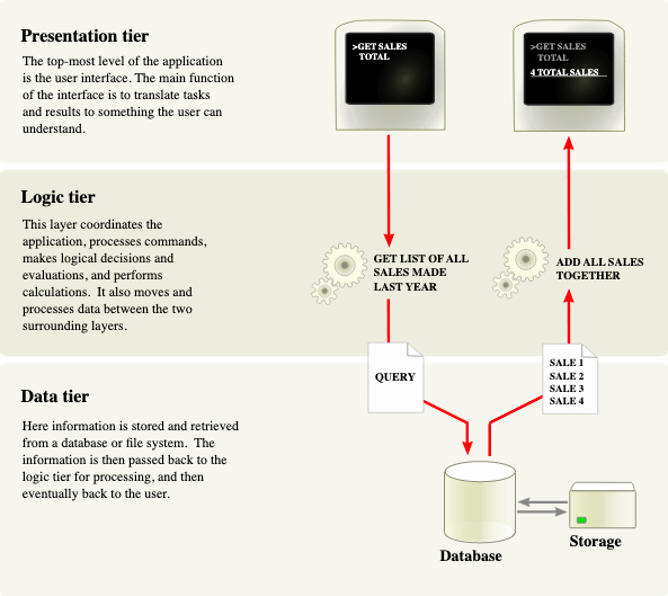
\includegraphics[width=12cm]{img/arsitekturOdoo.PNG}
	\captionof{figure}{Ilustrasi Arsitektur Odoo}
	\label{fig:asd}
\end{center}

Pada tingkatan paling atas yaitu tampilan(presentation tier), tampilan ini yang akan berinteraksi langsung dengan pengguna yang menggunakan aplikasi. Tampilan ini dibangun dengan teknologi web yaitu HTML5, Javascript, dan CSS. Tingkatan dibawahnya yaitu aturan bisnis(logic tier) yang berisi instruksi yang memproses data dan memberikan tanggapan dari interaksi kepada pengguna. Aturan pada Odoo hanya ditulis dalam bahasa pemrograman Python. Sedangkan pada tingkat paling bawah adalah tempat penyimpanan menggunakan DBMS(Database Management System), Odoo hanya bisa mendukung database PostgreSQL.\\

Odoo memiliki struktur kode yang dibentuk sebagai module untuk setiap fiturnya. Sehingga dari sisi server dan client memiliki hubungan yang disatukan menjadi satu paket tersendiri. Dimana module adalah koleksi dari fungsi dan data untuk menyelesaikan satu tujuan. Modul pada Odoo bisa ditambahkan, diganti, diubah untuk menyesuaikan kebutuhan bisnis. Dimana pada pengguna module dilambangkan dengan nama Apps, tetapi tidak semua module adalah Apps. Modules juga bisa direfrensikan sebagai addons.\\

\begingroup
\setlength{\LTleft}{-20cm plus -1fill}
\setlength{\LTright}{\LTleft}
\begin{small}
	\begin{longtable}{|p{3cm}|p{5cm}|p{5cm}|}
		\caption{Komposisi dari Module pada aplikasi Odoo}\\
		\hline
		\textbf{Elemen} & \textbf{Keterangan} & \textbf{Contoh}\\
		\endfirsthead
		
		\hline
		    Business Objects
		  & Object yang akan digunakan di module dimana setiap attribute secara otomatik dipetakan ke kolom database dengan ORM
		  & File python yang memiliki class\\
		\hline  
		Objects Views
		  & Menangani bagaimana data ditampilkan di pengguna. Seperti visualisasi form, list, kanban dan lainnya
		  & Berupa file XML dengan struktur yang sudah ditentukan Odoo\\
		\hline
		Data Files
		  & Mengelola bagaimana model data seperti laporan, konfigurasi data, data contoh dan lainnya
		  & Berupa file XML atau CSV\\
		\hline
		Web Controllers
		  & Menangani permintaan dari browser/client
		  & File python yang memiliki class namun merupakan turunan dari class odoo.http.Controller\\
		\hline
		  Static Web Data
		  & File yang digunakan hanya ditampilkan kepada client di website
		  & File gambar, File CSS, dan File JavaScript\\
		 \hline  
	\end{longtable}
\end{small}
\endgroup

Struktur database yang dibentuk pada konfigurasi umum di Odoo memiliki jumlah tabel ±566 tabel, tabel ini merupakan keseluruhan dari aplikasi dimana dapat diidentifikasi 31 tabel utama yang digunakan pada aplikasi. Berikut adalah diagram dari database yang dibuat dengan alat DBeaver Visualize, dengan attribute hanya sebuah key dari tabel. \\
\begin{center}
	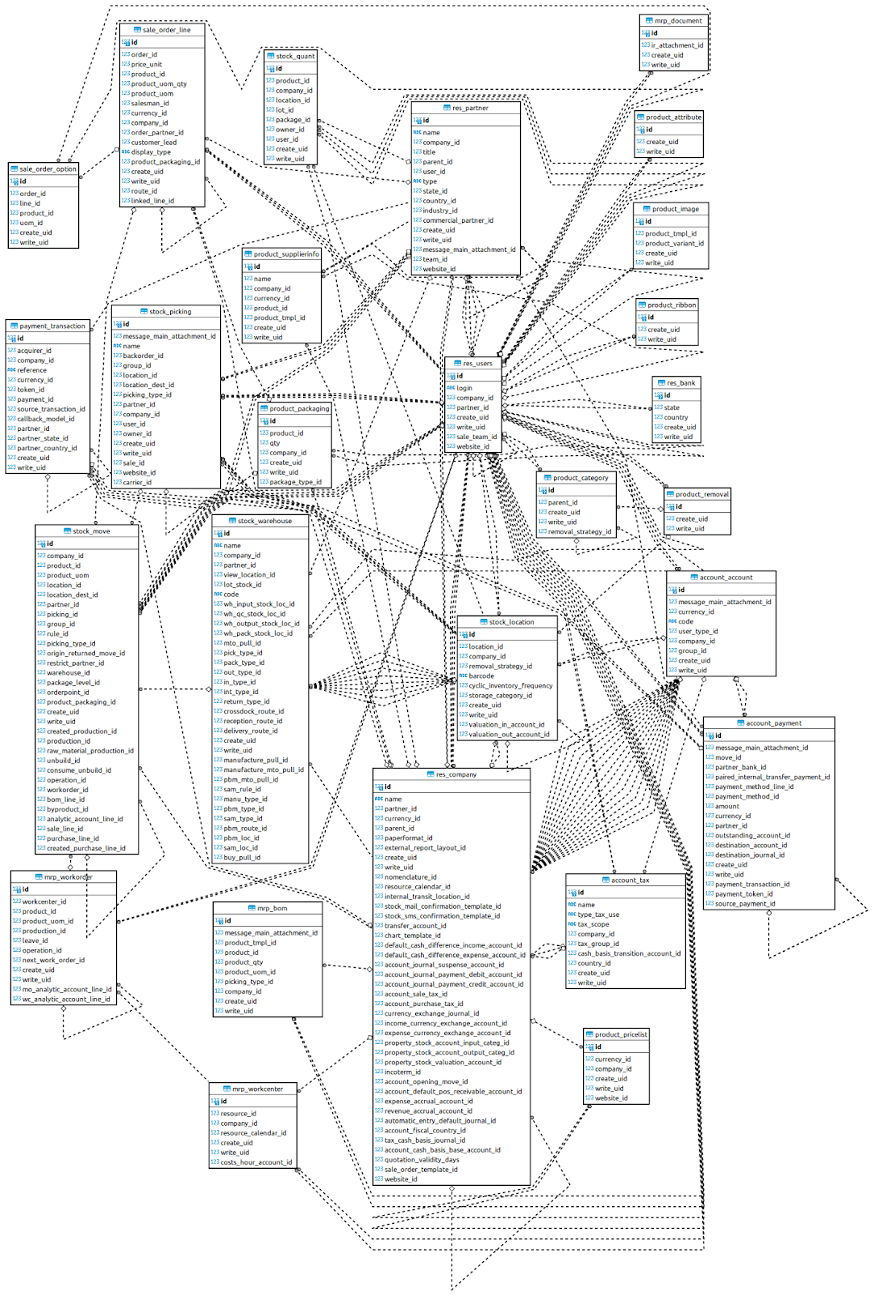
\includegraphics[width=14cm]{img/DatabaseOdoo.png}
	\captionof{figure}{Diagram Database Odoo}
	\label{fig:asd}
\end{center}




	
	\setcounter{page}{1}
	%-----------------------------------------------------------------------------%
\chapter{ANALISIS DAN PERANCANGAN SISTEM}
%-----------------------------------------------------------------------------%
\vspace{4.5pt}

Pada bab ini menjelaskan analisis masalah yang diatasi, alur kerja dari perangkat lunak yang dikembangkan, arsitektur dan metode yang digunakan serta hasil evaluasi.\\

\section{Analisis Masalah}
Arsitektur ERP yang digunakan pada Odoo yaitu arsitektur monolitik, seperti yang sudah dijelaskan pada landasan teori. Arsitektur monolitik memiliki kelemahan dan permasalahan yang bisa diselesaikan dengan arsitektur \textit{microservice}.

Namun untuk melakukan perubahan arsitektur harus dilakukan dekomposisi, proses dekomposisi sendiri tidak mudah karena proses dekomposisi masih membutuhkan analisis secara manual dan untuk mengidentifikasi \textit{service} sulit karena banyaknya pendekatan dan pertimbangan.

Pada penelitian ini menggunakan pendekatan \textit{Hierarchical Clustering} untuk membantu menemukan \textit{service} yang tepat, di mana \textit{Hierarchical Clustering} memberikan rekomendasi bagaimana pengelompokan \textit{service} berdasarkan pemilihan partisi.

Proses dimulai dari melalukan analisis kode seperti \textit{Call Graph} yang dihasilkan dari kode aplikasi Odoo. Hasil analisis kode di ekstraksi menjadi matriks untuk dilakukan \textit{Hierarchical Clustering}. \textit{Linkage} yang digunakan dalam melakukan \textit{Hierarchical Clustering} yaitu \textit{single}, \textit{complete}, dan \textit{average}, kemudian  Partisi  dipilih melalui nilai secara struktural yaitu nilai \textit{coupling}  dan \textit{cohesion}. Hasil terbaik dari \textit{clustering} disampling untuk diimplementasikan menjadi \textit{service}, penelitian ini akan menggunakan strategi dengan pola \textit{strangle fig } dan \textit{branch by abstraction} untuk memecah kode di monolitik.

\section{Kerangka Pemikiran}
\begin{center}
	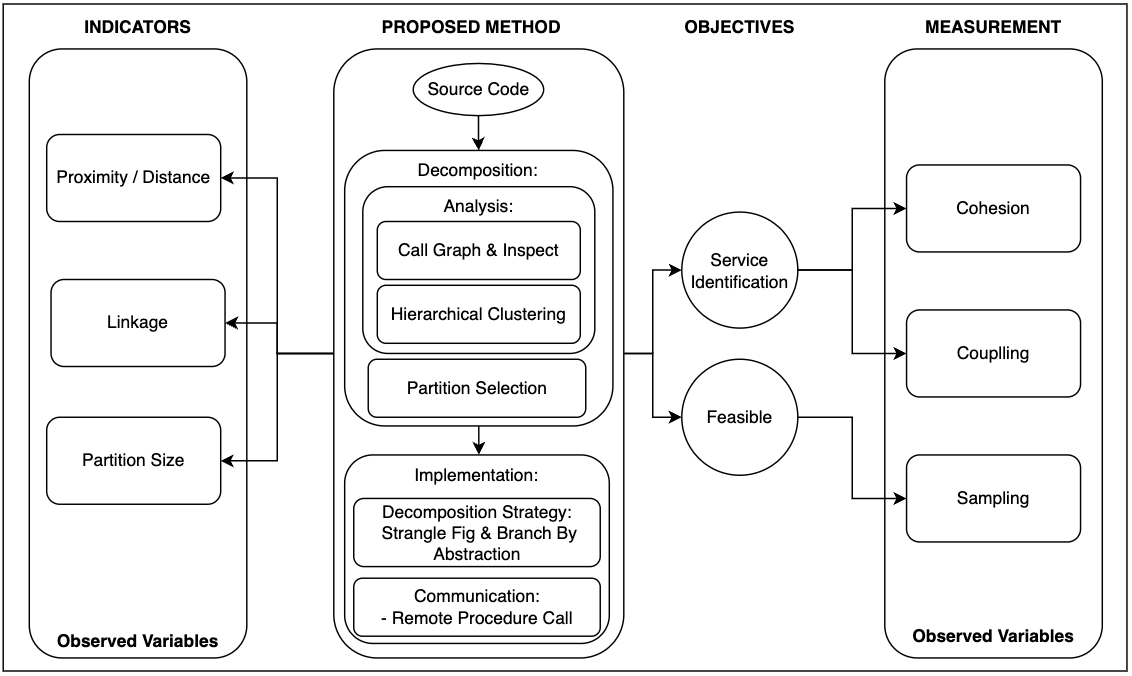
\includegraphics[width=14cm]{img/bab_3/KerangkaPemikiran.png}
	\captionof{figure}{Kerangka Pemikiran}
	\label{fig:kerangka_pemikiran}
\end{center}

Penelitian akan dimulai dengan menggunakan kode sumber aplikasi yang dibuat dengan monolitik. Kode sumber dilakukan proses dekomposisi yaitu dengan analisis seperti mencari objek beserta atributnya, untuk mencari keterhubungan lebih lanjut tentang objek maka dilakukan pencarian pada fungsi-fungsi sehingga terbentuklah \textit{call graph} yang menunjukkan bagaimana keterhubungan masing-masing objek di aplikasi.

Dari \textit{graph} yang sudah dibuat akan dilakukan pengelompokan dengan algoritma \textit{Hierarchical Clustering}. Pendekatan algoritma yang digunakan pada penelitian ini yaitu agglomerative, selain itu ditentukan cara menghitung kedekatan antara objek dan pemilihan algoritma \textit{Linkage}. Metode \textit{linkage} yaitu menentukan jarak atau kemiripan antara semua objek. Untuk menentukan jarak ini bisa dengan rata-rata, maximum, dan minimum. 

Pengelompokan dari \textit{Hierarchical Clustering} akan dipilih dengan mencari nilai \textit{cohesion} terendah dan  nilai \textit{coupling} tertinggi. Di mana \textit{coupling} mengevaluasi tingkat ketergantungan langsung dan tidak langsung antar objek. Semakin banyak dua objek menggunakan metode masing-masing semakin mereka menjadi satu kesatuan. Sedangkan  \textit{cohesion} akan mengevaluasi kekuatan interaksi antar objek. Biasanya, dua objek atau lebih menjadi interaktif jika metodenya menggunakan metodenya satu sama lain. Dengan membandingkan nilai  \textit{coupling}, \textit{cohesion}, \textit{linkage} dan ukuran partisi maka dapat diketahui kelompok service yang ideal.

Selain itu, untuk mengetahui apakah hasil \textit{clustering} relevan dan dapat diimplementasikan maka dilakukan sampling yang berjumlah 2 service dari kelompok service yang ideal. Untuk menerapkannya pemecahan dimulai dari pemecahan kode yang menggunakan strategi dekomposisi \textit{strangle fig } dan \textit{branch by abstraction}. Untuk metode komunikasinya antara \textit{service} yaitu dengan Remote Procedure Call(RPC) dan untuk mengelola datanya, setiap \textit{service} memiliki databasenya masing-masing.\\

\section{Urutan Proses Global}
\begin{center}
	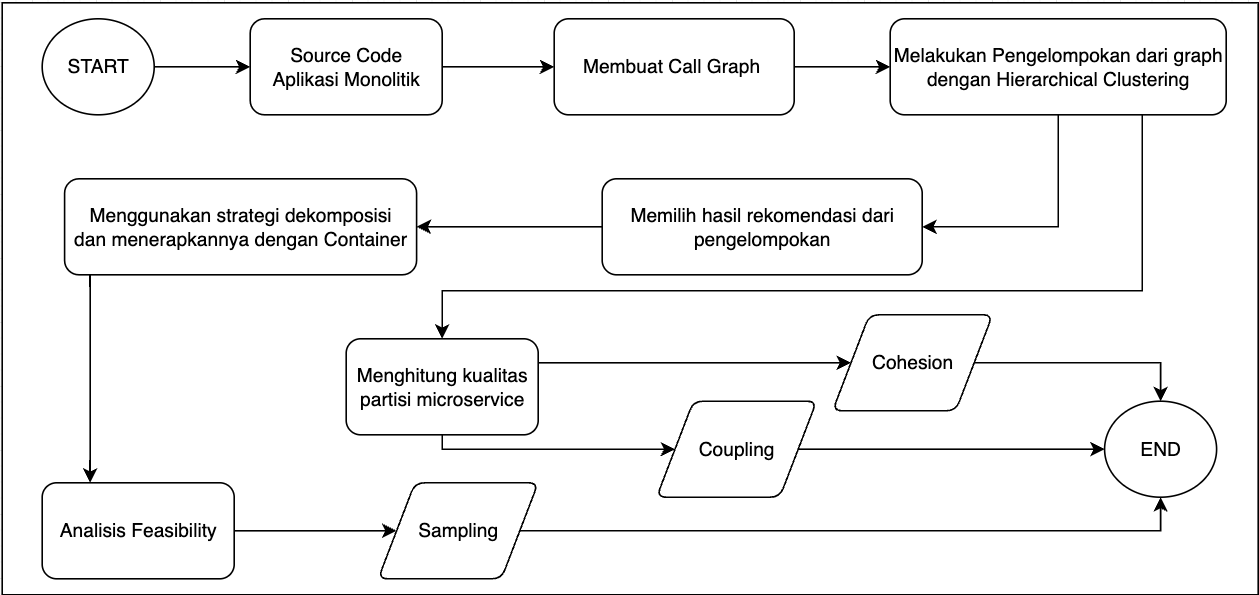
\includegraphics[width=14cm]{img/bab_3/FlowchartProsesGlobal.png}
	\captionof{figure}{Diagram Flowchart Proses Global }
	\label{fig:proses_Global}
\end{center}

\subsection{Proses Clustering}

\subsubsection{Pengambilan Source Code}
Aplikasi ERP Odoo merupakan aplikasi berlisensi open source, kode program dapat diunduh melalui situs repository Odoo. Pada tugas akhir ini menggunakan Odoo versi 16 dengan status pengujian lulus. Agar kode program dapat berjalan dengan lancar maka diperlukan proses installasi library, module dan Package yang digunakan dari file requirement.txt
\begin{center}
	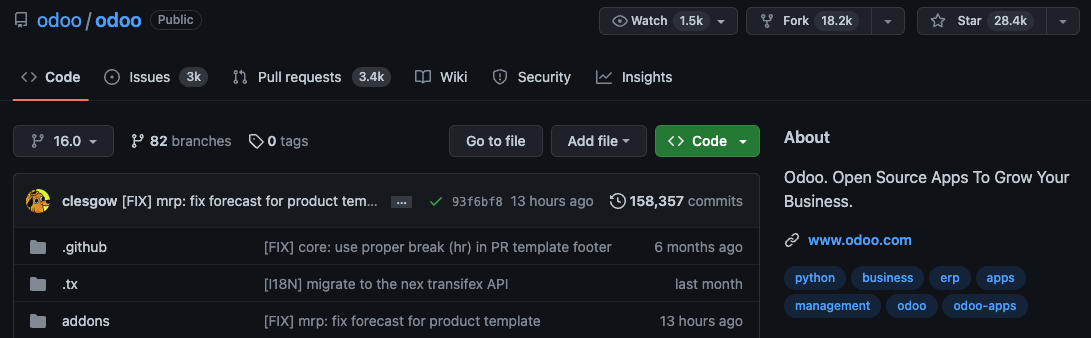
\includegraphics[width=14cm]{img/bab_3/github.png}
	\captionof{figure}{Source Code Aplikasi Odoo pada git repository}
	\label{fig:github_ss}
\end{center}

\subsubsection{Pembuatan \textit{Call Graph}}
Pada tugas akhir ini menggunakan tools PyCG untuk menghasilkan \textit{call graph} dalam bentuk format JSON. Terdapat target folder yang harus dianalisis oleh PyCG \textit{call graph} yaitu folder 'odoo/addons" atau package 'odoo.addons'. Pemilihan folder ini dikarenakan folder/package lainnya tidak memiliki hubungan mengenai proses bisnis. Untuk menghemat waktu pembuatan \textit{call graph} maka folder test dan l10n (localization) tidak dianalisis.  

\textit{Entry point} untuk \textit{tools} PyCG adalah semua file di target folder dengan ekstensi file .py serta ditentukan package yang ingin diolah menjadi \textit{call graph}. Proses eksekusi dilakukan melalui terminal. \textit{Call graph} yang dihasilkan berisi \textit{call} yang berasal dari file .py yang ditentukan sebelumnya dan semua module yang terhubungan dari target. Semua module ini bisa diluar dari target module apabila keterhubungan itu terus berlanjut. PyCG hanya bisa menghasilkan \textit{call graph} tanpa informasi mengenai jumlah pemanggilan dan urutan pemanggilan.

\begin{center}
	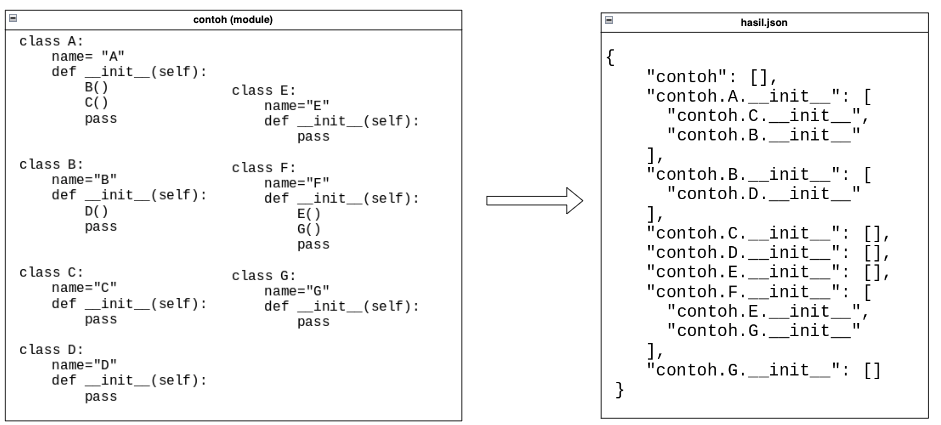
\includegraphics[width=13cm]{img/bab_3/soToCG.png}
	\captionof{figure}{Proses Pembuatan \textit{Call Graph} dengan PyCG}
	\label{contoh_json_pycg}
\end{center}

Proses ekstraksi json yang dihasilkan dari tools PyCG berupa file JSON yang dinamakan berdasarkan argrument yang diberikan sebelumnya seperti 'addons.json'. File JSON diubah menjadi \textit{graph} yang direpresentasikan dalam bentuk \textit{adjacency} list di Python.

\subsubsection{Ekstraksi Dependency Model}
Keterbatasannya informasi \textit{call graph} yang dihasilkan dari PyCG, sehingga tugas akhir ini menggunakan library Python yaitu 'inspect' untuk menganalisis objek secara run-time. Hal ini disebabkan Python adalah bahasa pemrogram dinamik di mana pengecekan tipe data dilakukan secara 'run-time'. Ekstrasi ini difokuskan pada module yang memiliki proses bisnis seperti module addons. Dari gambar 3.5 bisa diketahui penggunaan inspect bisa menemukan atribut apa saja dan nilainya dari atribut pada objek. 

\begin{center}
	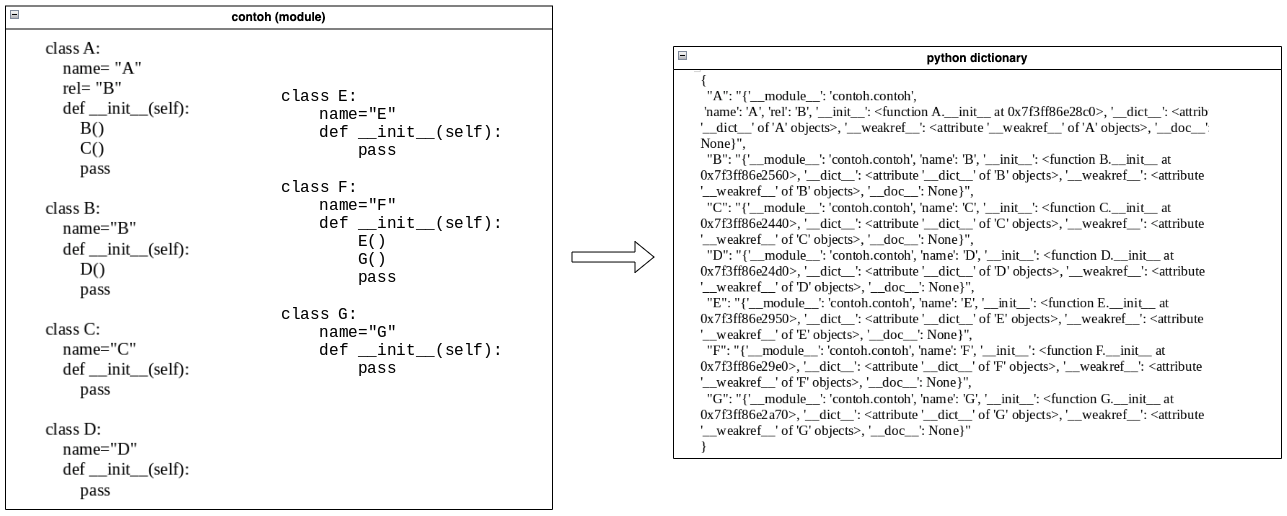
\includegraphics[width=13cm]{img/bab_3/inspectSample.png}
	\captionof{figure}{Penggunaan 'inspect' untuk melihat objek Python lebih mendalam}
	\label{contoh_inspectSample}
\end{center}

Object yang dianalisis yaitu \textit{class} yang merupakan turunan dari \textit{class} odoo.models.MetaModel, di mana \textit{class} MetaModel memiliki properti seperti  name, \_inherits , \_inherit, dan comodel\_name. Hasil ekstrasi dependency model digabungkan melalui nama module PyCG.

\subsubsection{Pengabungan dan Optimisasi Hasil Ekstraksi}
Graph yang dihasilkan dari proses ekstrasi dipisahkan antara module eksternal dan module internal. Module yang digunakan untuk pengelompokan adalah module internal, setiap \textit{call} yang dilakukan memiliki nama \textit{call} yang berupa gabungan antara nama fungsi / \textit{class} / module /file di kode program. PyCG tidak memberikan informasi apakah nama \textit{call} tersebut berupa tipe apa, untuk itu pengelompokan dilakukan secara campuran yaitu berdasarkan module dan file, yang dikelompokkan menjadi file hanya addons base.

Nama \textit{call} yang disatukan menjadi module adalah \textit{call} yang memiliki awalan(root) addons atau odoo/addons dan nama \textit{call} yang disatukan dengan file adalah nama \textit{call} selain addons. Call yang dikelompokkan memiliki nilai agregasi dari jumlah \textit{call}. Jumlah \textit{call} dapat digunakan sebagai weight yang dapat menunjukkan kekuatan antara \textit{call} satu sama lain, proses ini membentuk \textit{call} baru yang lebih ringkas dan relevan dalam bentuk \textit{graph}. 

Pada gambar \ref{fig:dg_al} dapat dilihat hasil dari graph yang dihasilkan dari contoh PyCG dan Inspect sebelumnya. Graph yang digunakan merupakan directed sehingga setiap pemanggilan berlaku untuk satu arah. Graph ini dapat diubah menjadi bentuk dictionary sebagai \textit{adjacency} list, tujuannya agar pengaksesan dan pencarian node lebih cepat dan mudah dilakukan. Setiap relasi memiliki jumlah berapa kali node lain dipanggil dari node tersebut.

\begin{center}
	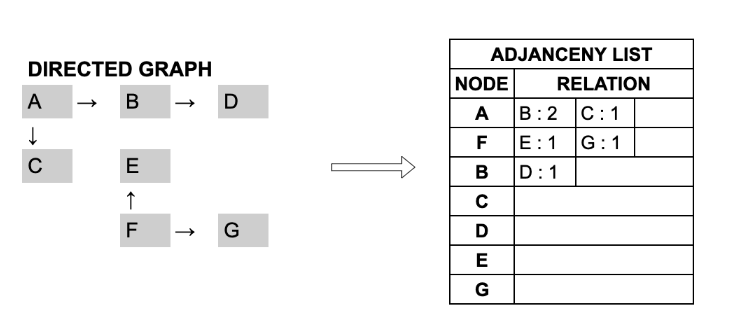
\includegraphics[width=13cm]{img/bab_3/dg_al.png}
	\captionof{figure}{Graph dan Adjanceny List}
	\label{fig:dg_al}
\end{center}

\subsubsection{Hierarchical Clustering}
Graph yang berbentuk \textit{Adjacency} list diubah menjadi \textit{adjacency} \textit{matrix}, proses normalisasi data dilakukan pada matriks. Tujuan normalisasi data agar nilai \textit{weight}(jumlah \textit{call}) dari relasi berkisar dari 1 hingga 0. Semakin banyak jumlah \textit{call} dilakukan maka nilai mendekati 1,kemudian matriks tersebut dibuat menjadi \textit{Distance} \textit{Matrix}, rumus jarak yang digunakan ada 2 yaitu Jaccard dan Struktural Similarity. Jaccard menghasilkan hasil yang bagus pada remodularisasi perangkat lunak dan Struktural Similarity digunakan untuk melihat kedekatan dari sisi intesitas panggilan antara module.

Berikut pada gambar \ref{fig:weight_normal_mat} dilakukan proses perubahan dari \textit{adjacency} list menjadi \textit{adjacency} \textit{matrix} yang memiliki bobot. Kemudian dilakukan normalisasi kolom, dimana setiap nilai dibandingkan dengan nilai maximum dan nilai minimum pada kolom yang sama. 

\begin{center}
	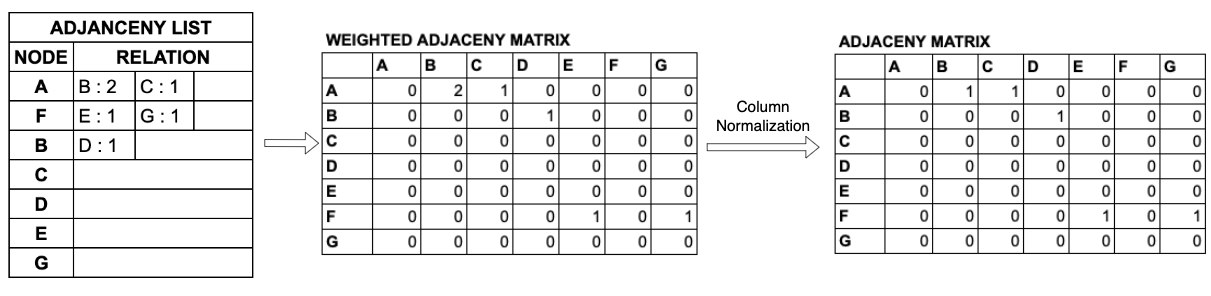
\includegraphics[width=14cm]{img/bab_3/weight_normal_mat.png}
	\captionof{figure}{Perubahan dari \textit{Adjacency} List menjadi \textit{Adjacency} \textit{Matrix}}
	\label{fig:weight_normal_mat}
\end{center}

Proses perhitungan jarak antara 2 objek dilakukan dari \textit{adjacency} \textit{matrix} dengan pola urutan berbentuk matriks segitiga bawah. Dengan ini perbandingan pertama kali dilakukan di baris ke-2(index=1) di kolom ke-1(index=0) dan berakhir pada baris ke-n(jumlah objek) di kolom  ke n-1. Pada contoh di \ref{fig:distance_detail} dijelaskan untuk perhitungan total jarak pada objek B dan A. Sebelum dilakukan perhitungan matriks terlebih dahulu sisi diagonal diberi nilai 1 untuk mengartikan bahwa objek memiliki hubungan dengan dirinya sendiri.  Perhitungan dimulai menghitung kimiripan jaccard, jaccard menghasilkan kemiripan dari jumlah interseksi dibagi jumlah union pada objek. Perhitungan selanjutnya Similarity Struktural menghitung dengan mempertimbangkan jumlah sisi panggilan kedua objek yaitu baris ke-1(index=0), baris ke-2(index=1) dan jumlah sisi panggilan keluar kedua objek yaitu kolom  ke-1(index=0) dan kolom ke-2(index=1). Hasil kemiripan Similarity Struktural dan Jaccard dirata-ratakan untuk menjadi nilai akhir kemiripan objek.

\begin{center}
	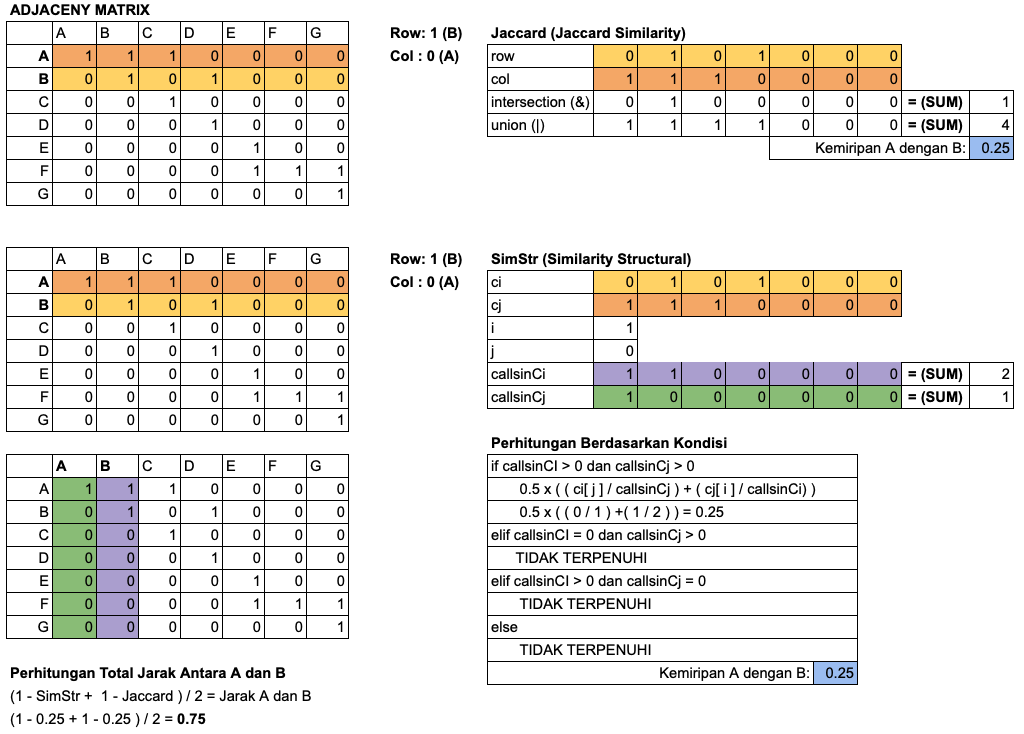
\includegraphics[width=14cm]{img/bab_3/distance_detail.png}
	\captionof{figure}{Perhitungan Jarak}
	\label{fig:distance_detail}
\end{center}

\begin{center}
	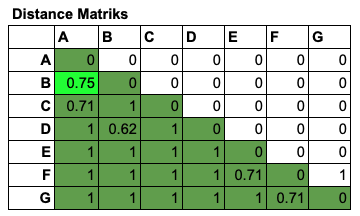
\includegraphics[width=7cm]{img/bab_3/distance_final.png}
	\captionof{figure}{Hasil Akhir Jarak}
	\label{fig:asd}
\end{center}

Distance \textit{Matrix} / Matriks kedekatan dapat dilihat nilai dengan ilustrasi Heatmap, di mana sumbu x dan y adalah semua module dan nilai kedekatannya dengan module lainnya. Semakin terang warna menunjukkan hubungan yang kuat antara module, perlu diketahui bahwa \textit{distance} \textit{matrix} merupakan matriks segitiga. Pada tugas akhir ini menggunakan library SciPy untuk melakukan proses \textit{clustering} yang memiliki fungsi \textit{Hierarchical Clustering}.

\begin{center}
	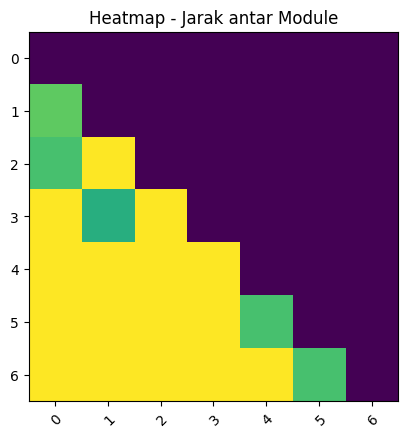
\includegraphics[width=7cm]{img/bab_3/heatmap.png}
	\captionof{figure}{Heatmap yang dihasilkan dari \textit{Distance} \textit{Matrix}}
	\label{fig:asd}
\end{center}

Pemilihan pengelompokan dengan hierarchical agglomerative \textit{clustering} dibandingkan Paritition \textit{clustering} karena tidak mudah untuk mengetahui jumlah ideal \textit{cluster}. Untuk menentukan metode \textit{linkage} tugas akhir ini menggunakan \textit{single} lingkage, \textit{average} \textit{linkage}, dan \textit{complete} lingkage. Hasil dari masing-masing lingkage dipilih jumlah partisi yang ideal untuk \textit{microservice}. Penggunaan \textit{single} lingkage memiliki kecenderungan menghasilkan banyak partisi yang berisi modul sedikit tetapi ada satu partisi memiliki banyak module sedangkan \textit{complete} \textit{linkage} menghasilkan partisi yang memiliki jumlah modul yang sama dengan partisi lainnya. Untuk \textit{Average} lingkage menghasilkan bentuk partisi di antara \textit{complete} lingkage dan \textit{single} lingkage.

Pada gambar \ref{fig:hc_detail_1} dijelaskan mengenai proses perhitungan \textit{Hierarchical Clustering} dengan \textit{distance} matriks yang sebelumnya sudah dihitung. Perhitungan \textit{Hierarchical Clustering} terdapat 5 bagian besar yaitu pertama memiliki objek pertama (urutan pertama), ke-2 mencari objek lainnya yang terdekat berdasarkan \textit{distance} \textit{matrix}, ke-3 mengabungkan objek yang terdekat dengan objek yang pertama dan membuat kelompok baru dari objek tersebut, ke-4 memperbaharui nilai jaraknya pada kelompok baru / partisi menggunakan \textit{linkage}. Penggunaan \textit{linkage} akan membandingkan 2 nilai objek yaitu dari nilai objek yang baru dan nilai objek yang sebelumnya (yang terdapat di \textit{distance} matriks) seperti min memilih nilai yang lebih rendah, \textit{complete} memilih nilai yang lebih tinggi, dan \textit{average} melakukan nilai rata-rata dari 2 nilai objek. Langkah terakhir bila sudah tidak ada objek tersisa maka perhitungan berhenti bila masih ada maka dilajukan kembali proses yang ke-2.

\begin{center}
	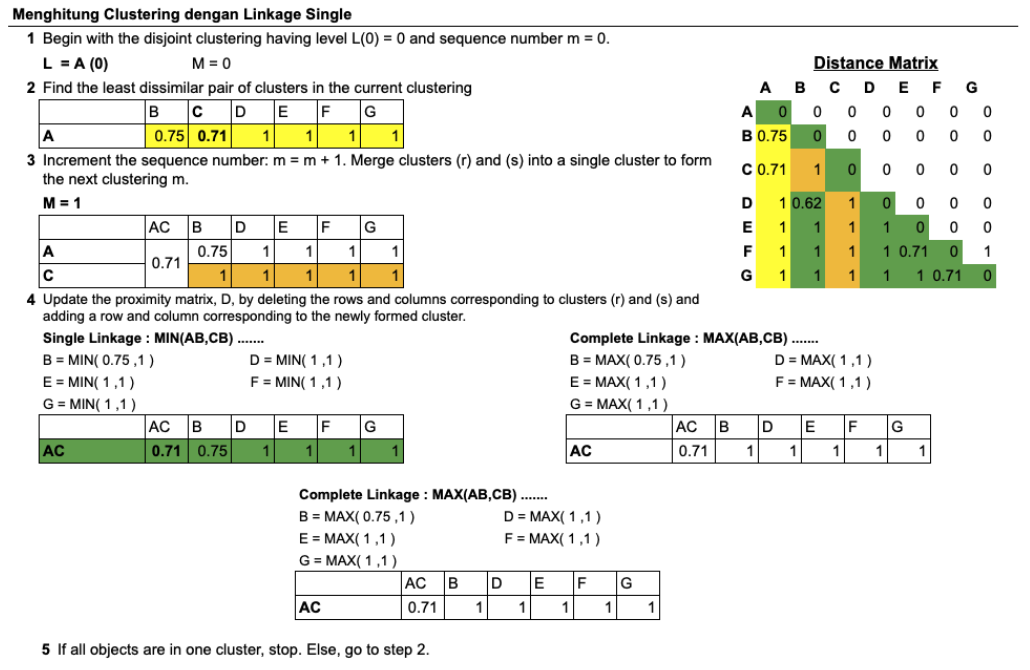
\includegraphics[width=14cm]{img/bab_3/hc_detail_1.png}
	\captionof{figure}{Proses Perhitungan \textit{Hierarchical Clustering}}
	\label{fig:hc_detail_1}
\end{center}

\begin{center}
	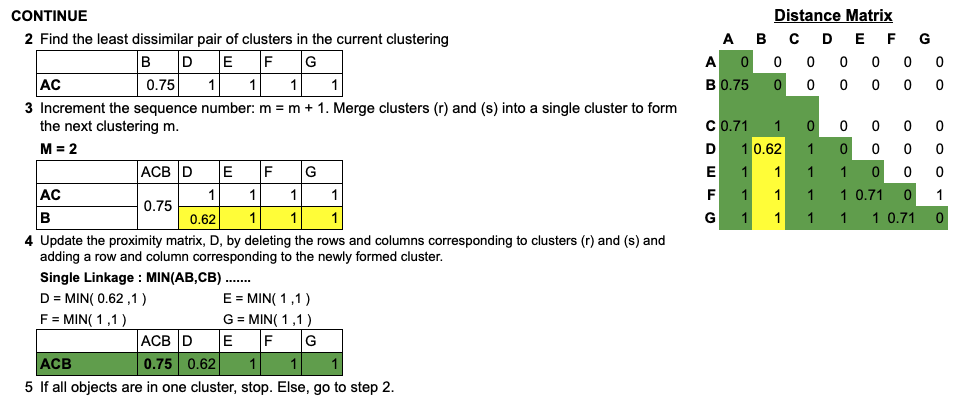
\includegraphics[width=14cm]{img/bab_3/hc_detail_2.png}
	\captionof{figure}{Lanjutan Proses Perhitungan \textit{Hierarchical Clustering}}
	\label{fig:hc_detail_2}
\end{center}

\begin{center}
	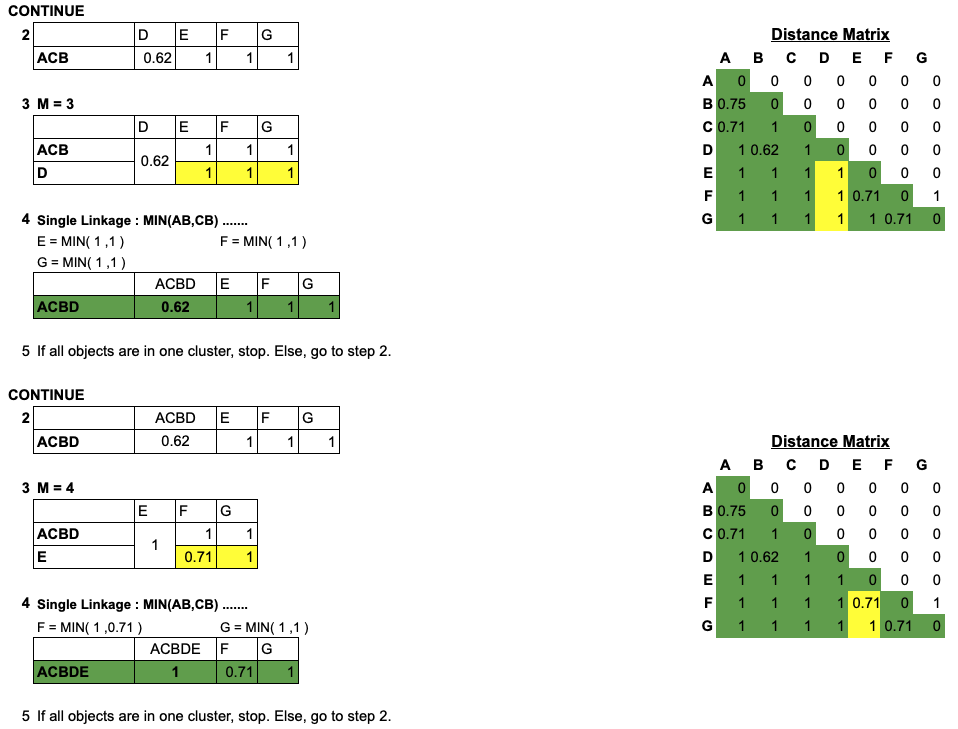
\includegraphics[width=14cm]{img/bab_3/hc_detail_3.png}
	\captionof{figure}{Lanjutan Proses Perhitungan \textit{Hierarchical Clustering}}
	\label{fig:hc_detail_3}
\end{center}

\begin{center}
	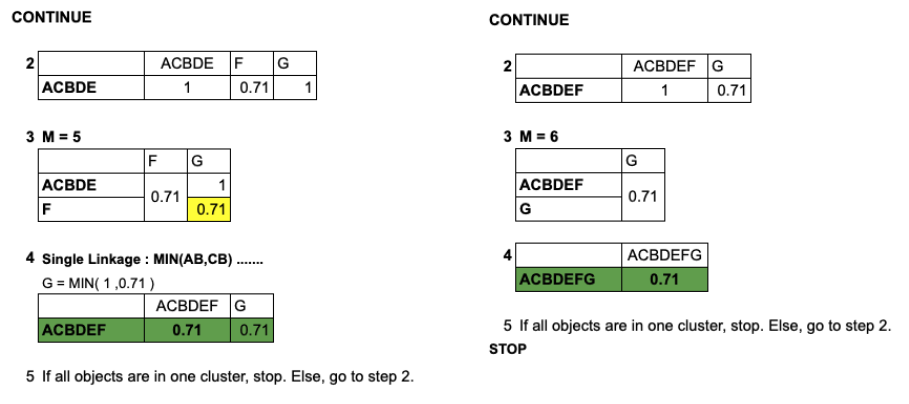
\includegraphics[width=14cm]{img/bab_3/hc_detail_4.png}
	\captionof{figure}{Lanjutan Proses Perhitungan \textit{Hierarchical Clustering}}
	\label{fig:hc_detail_4}
\end{center}

Hasil pengelompokan dapat ditampilan dalam bentuk dendogram.  Di mana pengelompokan dari setiap \textit{linkage} memiliki dampak berbeda yang bisa dilihat dari bentuk dan nilai kedekatan antar partisi melalui dendogram dan bentuk relasi. Angka gabungan yang ditampilan pada dendogram merupakan jarak \textit{linkage} yang dihitung dari proses perhitungan \textit{Hierarchical Clustering} sebelumnya.

\begin{center}
	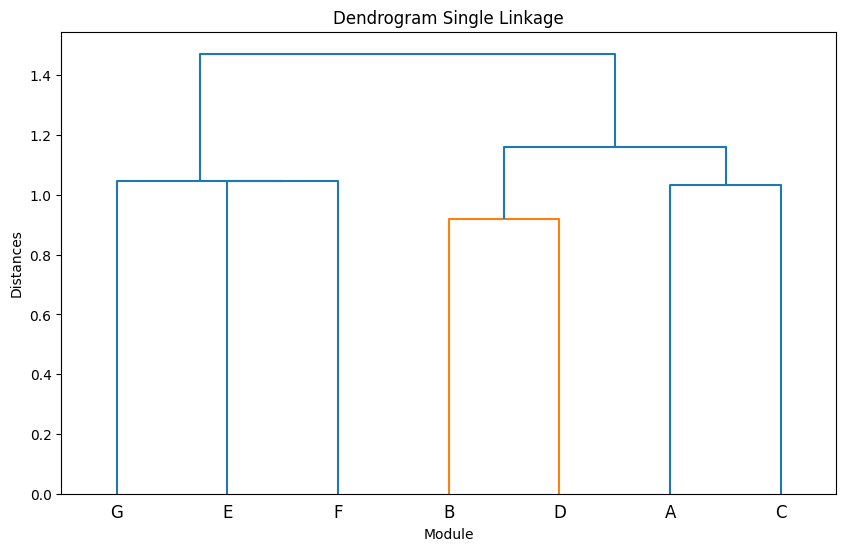
\includegraphics[width=11cm]{img/bab_3/singleLink.png}
	\captionof{figure}{Dendogram \textit{Single} \textit{Linkage}}
	\label{fig:asd}
\end{center}
\begin{center}
	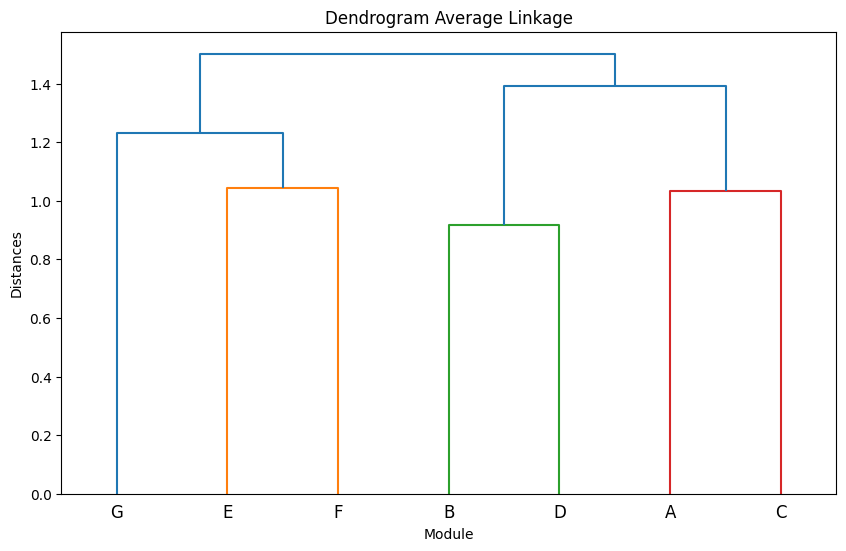
\includegraphics[width=11cm]{img/bab_3/averageLink.png}
	\captionof{figure}{Dendogram \textit{Average} \textit{Linkage}}
	\label{fig:asd}
\end{center}
\begin{center}
	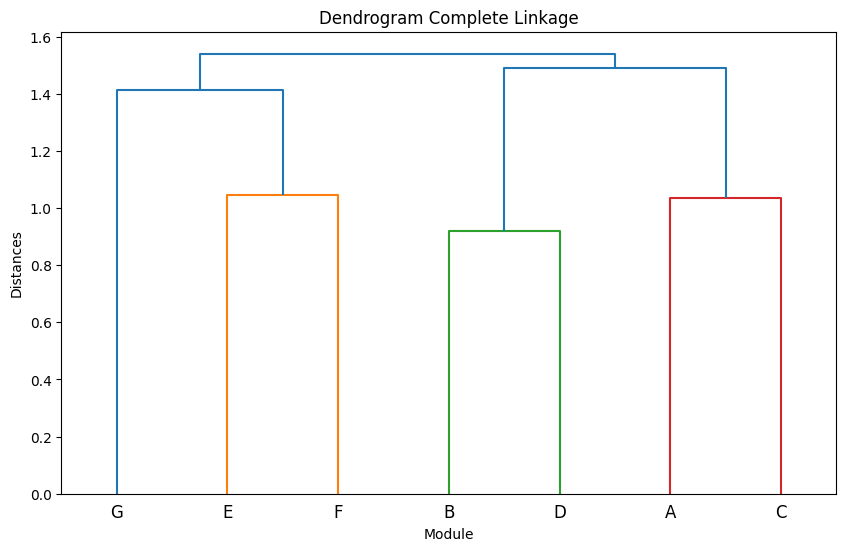
\includegraphics[width=11cm]{img/bab_3/completeLink.png}
	\captionof{figure}{Dendogram \textit{Complete} \textit{Linkage}}
	\label{fig:asd}
\end{center}

\subsubsection{Pemilihan Partisi}
Pemilihan jumlah partisi perlu dilakukan dengan perhitungan yang dapat menentukan jumlah \textit{service} yang ideal. Microservice yang ideal memiliki nilai \textit{coupling} yang rendah dan nilai \textit{cohesion} yang tinggi. Untuk itu tugas akhir ini menentukan partisi dengan nilai struktural yang menggunakan persamaan 2.2 dan tidak memperhitungkan nilai \textit{coupling} external karena addons pada Odoo dibuat dengan framework Odoo. Hubungan module luar seperti library umumnya dilakukan oleh framework Odoo sendiri bukan oleh addons.

Untuk pemilihan partisi harus mempertimbangkan nilai \textit{cohesion}, nilai \textit{coupling}, jumlah \textit{service}, dan apakah \textit{service} tersebut seimbang. Partisi yang akan menjadi \textit{service} diharapkan bisa independen. 

Proses pemilihan partisi dimulai dari pemotongan tree dari hasil \textit{Hierarchical Clustering} sebelumnya. Pemotongan dilakukan berdasarkan jumlah cluster / partisi, kemudian  dipetakan dalam bentuk directed graph untuk menyusun kelompok partisi yang berisi relasi objek-objek / modul. Didalam node graph setiap hubungan module diluar dari partisinya akan dihitung sebagai panggilan ke luar dan hubungan antar module yang masih didalam  dihitung sebagai panggilan internal partisi.

\begin{center}
	\includegraphics[width=14cm]{img/bab_3/eval_detail1.png}
	\captionof{figure}{Proses pemotongan tree dan perubahan menjadi \textit{Adjacency} \textit{Matrix}  dengan \textit{linkage} \textit{single} sejumlah 3 partisi}
	\label{fig:asd}
\end{center}

Module juga memiliki panggilannya internal masing-masing sebelumnya karena didalam module bisa berisi banyak sub-module lainnya, data ini disimpan dalam bentuk key-value dictionary. panggilan internal dibutuhkan untuk membuat kohesi yang benar dan panggilan eksternal (diluar partisi) digunakan untuk menghitung nilai coupling.  Pada tugas akhir ini menggunakan Structural and Behavioral Dependencies untuk mengevaluasi hasil partisi yang dihasilkan oleh \textit{Hierarchical Clustering}. Node graph diubah kembali menjadi \textit{Adjacency} \textit{Matrix} untuk memudahkan akses seperti komparasi hubungan antar partisi. 

\begin{center}
	\includegraphics[width=14cm]{img/bab_3/eval_detail2.png}
	\captionof{figure}{Proses perhitungan coupling dan cohesion }
	\label{fig:asd}
\end{center}

Berikut adalah hasil nilai \textit{coupling} dan \textit{cohesion} masing-masing jumlah \textit{cluster}. Semakin tinggi jumlah \textit{cluster} maka nilai \textit{coupling} akan meningkat dan begitu pula sebaliknya untuk nilai \textit{cohesion}. Dari contoh data ditemukan bahwa \textit{cluster} yang ideal berjumlah 2 \textit{service}, karena ketika semakin banyak jumlah \textit{service} maka nilai \textit{coupling} meningkat dan sebaliknya nilai \textit{cohesion} menurun.


\begin{center}
	\includegraphics[width=12cm]{img/bab_3/cohVScoup_single.png}
	\captionof{figure}{Perbandingan dari nilai Cohesion dan nilai Coupling dengan jumlah \textit{cluster}/partisi menggunakan \textit{Single} \textit{Linkage}}
	\label{fig:asd}
\end{center}

\pagebreak

\subsection{Dekomposisi Monolitik ke Microservice}
\subsubsection{Strategi Pemisahan Kode}
Odoo adalah aplikasi ERP berbasis web, tampilan pada Odoo bisa dibuka pada broser yang kompatibel. Odoo menggunakan pendekatan SPA (Single Page Application) dan adanya server rendering untuk menghasilkan HTML yang dinamik. Pada gambar \ref{fig:arsitektur_mono} terlihat bahwa aplikasi odoo merupakan aplikasi berbasis client-server.
\begin{center}
	\includegraphics[width=12cm]{img/bab_3/mono_ori.png}
	\captionof{figure}{Arsitektur di Monolitik} 
	\label{fig:arsitektur_mono}
\end{center}

Proses pemisahan membutuhkan \textit{reverse} \textit{proxy} yang dapat menghubungkan client dengan banyak server. Tujuan adanya \textit{reverse} \textit{proxy} agar \textit{client} hanya perlu mengetahui satu pintu masuk aplikasi yaitu \textit{reverse} \textit{proxy} itu sendiri dan tidak perlu mengetahui seluruh server yang ada di aplikasi.

\begin{center}
	\includegraphics[width=14cm]{img/bab_3/micro_proxy.png}
	\captionof{figure}{Arsitektur di Microservice}
	\label{fig:arsitektu_micro}
\end{center}

Berdasarkan landasan teori terdapat beberapa strategi pemisahan kode aplikasi monolitik, pada tugas akhir ini akan menggunakan 2 strategi yaitu pola \textit{Strangle} dan pola Branch by Abstraction. Pola \textit{Strangle} diterapkan karena pendekatan ini umum diterapkan dan lebih mudah pada suatu aplikasi yang sudah besar, dengan pola ini aplikasi monolitik bisa berdiri bersamaan dengan \textit{service} yang ingin dibangun atau dimigrasi. 

Tugas Akhir ini menggunakan \textit{API Gateway} Kong \textit{(off-the-shelf)} karena Kong sudah memiliki fitur yang lengkap pada kasus migrasi aplikasi monolitik ke \textit{microservice}. Fitur itu berupa kemampuan untuk redireksi url untuk menerapkan proses \textit{strangle}, pemantauan \textit{service}, dan memiliki performa yang baik.

\begin{center}
	\includegraphics[width=10cm]{img/bab_3/strangelExMono.png}
	\captionof{figure}{Ilustrasi Struktur Module dan Keterhubungannya di Aplikasi Monolitik}
	\label{fig:asd}
\end{center}

Terdapat 3 langkah utama dalam menerapkan pola \textit{strangle} yaitu memilih bagian yang ingin dipindahkan, memindahkan aplikasi menjadi \textit{service} yang berdiri sendiri, dan yang terakhir mengubah \textit{call} dari monolitik ke \textit{service} yang baru dibuat.
 
Untuk menghubungkan antara bagian yang sudah dipisah dari monolitik dengan bagian yang masih di monolitik maka diperlukan penerapan pola Branch by Abstraction. Terdapat dua bagian utama yaitu abstract dan adapter. Abstract berperan menggantikan bagian yang sudah pisah menjadi \textit{service} sehingga bagian lain di monolitik tidak terdampak dan Adapter adalah implementasi sesungguhnya yang menghubungkan antara \textit{service} dan aplikasi monolitik.

\begin{center}
	\includegraphics[width=12cm]{img/bab_3/strangelExMicro.png}
	\captionof{figure}{Penerapan Pola \textit{Strangle} dan Branch by Abstraction}
	\label{fig:asd}
\end{center}

Pemisahan kode mempengaruhi proses autentikasi, proses autentikasi pada aplikasi Odoo terdapat 2 cara yaitu melalui password atau API-Key. Odoo menyimpan sesi autentikasi di cookie namun bukan dalam format JSON Web Token (JWT) tapi bentuk HTTP session. Untuk itu diperlukan modifikasi pada sistem autentikasi yang menggunakan format JWT agar setiap \textit{service} tidak perlu menvalidasi berkali-kali apakah sesi itu valid. 

\begin{center}
	\includegraphics[width=14cm]{img/bab_3/stateDiagramLogin.png}
	\captionof{figure}{State Diagram pada proses login}
	\label{fig:asd}
\end{center}


\subsubsection{Komunikasi antar service}
Proses komunikasi antar \textit{service} dilakukan melalui JSON-RPC karena Odoo sudah memiliki untuk setiap addonsnya RPC ini bisa berupa XML atau JSON. Komunikasi ini melalui protokol  HTTP agar bisa akses oleh browser.  
\\
\subsubsection{Strategi Pemisahan \textit{database}}
Pemisahan \textit{database} dilakukan setelah dilakukan pemisahan kode karena pada Odoo sudah terdapat ORM yang mengelola \textit{database}. Ketika \textit{database} ingin dipisahkan maka pengaksesan \textit{database} monolitik  digunakan sebagai data access layer melalui API yang bisa berupa JSON-RPC.
\\ 


	
	\setcounter{page}{1}
	%-----------------------------------------------------------------------------%
\chapter{IMPLEMENTASI DAN PENGUJIAN}
%-----------------------------------------------------------------------------%

\vspace{4.5pt}

\section{Lingkungan Implementasi}
Mea tale aliquam minimum te. Eu mel putant virtute, essent inermis nominavi mea no. Laoreet indoctum sea te. Te scripta fabulas duo, pro doming recusabo voluptaria at. Cu sed numquam inciderint, ei minim altera disputando cum, te nec graeco maiorum convenire.\\
Cu mel putent rationibus dissentiet. Per vidisse scaevola oportere ei, qui solet molestie eu. Hinc diceret nominati per at, nec dico denique laboramus et. Legere regione his at, aeque decore in mei.Aliquam tincidunt a nulla ac posuere. Maecenas sapien mi, feugiat sit amet tellus at, dictum varius ante. Cras rutrum facilisis felis at hendrerit. Nullam eleifend sed lorem a iaculis. Donec ut odio at nisl molestie euismod quis et purus. Curabitur eu ex turpis. Etiam maximus metus non iaculis placerat. Sed in risus sodales, posuere elit in, eleifend tellus. Mauris at consectetur arcu. Integer fringilla eros mi, vel volutpat enim commodo ac.\\

\subsection{Spesifikasi Perangkat Keras}
Suspendisse ac porta diam, ut viverra ante. Aliquam mattis tincidunt diam in molestie. Sed auctor fermentum turpis, sed varius ante. Nulla rutrum, enim et efficitur dignissim, urna diam consequat purus, sit amet elementum nibh mauris ut tellus. Quisque interdum leo ligula, a volutpat mauris viverra ut. Fusce ac felis finibus, convallis ligula a, aliquam nunc. Quisque faucibus ligula et ornare finibus. Morbi maximus dolor vitae dolor tristique, eu sagittis metus auctor. Pellentesque quam lacus, ornare ut est ut, egestas auctor leo. Duis eros neque, mollis quis elit id, cursus egestas neque. Pellentesque ac sapien vitae nulla varius rhoncus. Orci varius natoque penatibus et magnis dis parturient montes, nascetur ridiculus mus. Etiam pharetra nisl et massa facilisis aliquet. Nulla sit amet quam enim. Nunc dictum pellentesque orci, at sollicitudin erat condimentum eu. Nullam mi dolor, vestibulum at lacinia quis, feugiat faucibus felis.\\

Suspendisse ac porta diam, ut viverra ante. Aliquam mattis tincidunt diam in molestie. Sed auctor fermentum turpis, sed varius ante. Nulla rutrum, enim et efficitur dignissim, urna diam consequat purus, sit amet elementum nibh mauris ut tellus. Quisque interdum leo ligula, a volutpat mauris viverra ut. Fusce ac felis finibus, convallis ligula a, aliquam nunc. Quisque faucibus ligula et ornare finibus. Morbi maximus dolor vitae dolor tristique, eu sagittis metus auctor. Pellentesque quam lacus, ornare ut est ut, egestas auctor leo. Duis eros neque, mollis quis elit id, cursus egestas neque. Pellentesque ac sapien vitae nulla varius rhoncus. Orci varius natoque penatibus et magnis dis parturient montes, nascetur ridiculus mus. Etiam pharetra nisl et massa facilisis aliquet. Nulla sit amet quam enim. Nunc dictum pellentesque orci, at sollicitudin erat condimentum eu. Nullam mi dolor, vestibulum at lacinia quis, feugiat faucibus felis.\\

\subsection{Spesifikasi Perangkat Lunak}
Suspendisse ac porta diam, ut viverra ante. Aliquam mattis tincidunt diam in molestie. Sed auctor fermentum turpis, sed varius ante. Nulla rutrum, enim et efficitur dignissim, urna diam consequat purus, sit amet elementum nibh mauris ut tellus. Quisque interdum leo ligula, a volutpat mauris viverra ut. Fusce ac felis finibus, convallis ligula a, aliquam nunc. Quisque faucibus ligula et ornare finibus. Morbi maximus dolor vitae dolor tristique, eu sagittis metus auctor. Pellentesque quam lacus, ornare ut est ut, egestas auctor leo. Duis eros neque, mollis quis elit id, cursus egestas neque. Pellentesque ac sapien vitae nulla varius rhoncus. Orci varius natoque penatibus et magnis dis parturient montes, nascetur ridiculus mus. Etiam pharetra nisl et massa facilisis aliquet. Nulla sit amet quam enim. Nunc dictum pellentesque orci, at sollicitudin erat condimentum eu. Nullam mi dolor, vestibulum at lacinia quis, feugiat faucibus felis.\\

\section{Implementasi Perangkat Lunak}
Mea tale aliquam minimum te. Eu mel putant virtute, essent inermis nominavi mea no. Laoreet indoctum sea te. Te scripta fabulas duo, pro doming recusabo voluptaria at. Cu sed numquam inciderint, ei minim altera disputando cum, te nec graeco maiorum convenire.\\
Cu mel putent rationibus dissentiet. Per vidisse scaevola oportere ei, qui solet molestie eu. Hinc diceret nominati per at, nec dico denique laboramus et. Legere regione his at, aeque decore in mei
Mea tale aliquam minimum te. Eu mel putant virtute, essent inermis nominavi mea no. Laoreet indoctum sea te. Te scripta fabulas duo, pro doming recusabo voluptaria at. Cu sed numquam inciderint, ei minim altera disputando cum, te nec graeco maiorum convenire.
Cu mel putent rationibus dissentiet. Per vidisse scaevola oportere ei, qui solet molestie eu. Hinc diceret nominati per at, nec dico denique laboramus et. Legere regione his at, aeque decore in mei.\\

\subsection{Implementasi \textit{Class}}
Cu sed numquam inciderint, ei minim altera disputando cum, te nec graeco maiorum convenire.
Cu mel putent rationibus dissentiet. Per vidisse scaevola oportere ei, qui solet molestie eu. Hinc diceret nominati per at, nec dico denique laboramus et. Legere regione his at, aeque decore in mei.\\

\subsubsection{\textit{Class} Nama\_Class\_1}
Cu sed numquam inciderint, ei minim altera disputando cum, te nec graeco maiorum convenire.
Cu mel putent rationibus dissentiet. Per vidisse scaevola oportere ei, qui solet molestie eu. Hinc diceret nominati per at, nec dico denique laboramus et. Legere regione his at, aeque decore in mei.\\

\subsubsection{\textit{Class} Nama\_Class\_2}
Cu sed numquam inciderint, ei minim altera disputando cum, te nec graeco maiorum convenire.
Cu mel putent rationibus dissentiet. Per vidisse scaevola oportere ei, qui solet molestie eu. Hinc diceret nominati per at, nec dico denique laboramus et. Legere regione his at, aeque decore in mei.\\

\subsection{Implementasi Numquam}
Cu sed numquam inciderint, ei minim altera disputando cum, te nec graeco maiorum convenire.
Cu mel putent rationibus dissentiet. Per vidisse scaevola oportere ei, qui solet molestie eu. Hinc diceret nominati per at, nec dico denique laboramus et. Legere regione his at, aeque decore in mei.\\

\section{Implementasi Nama\_Implementasi}
Lorem ipsum dolor sit amet, consectetur adipiscing elit. Donec ac felis dignissim, iaculis odio ut, euismod quam. Donec vestibulum pellentesque sem, eu aliquet purus lacinia ac. Nam porttitor auctor justo et lobortis. Orci varius natoque penatibus et magnis dis parturient montes, nascetur ridiculus mus. Sed et gravida neque. Praesent commodo aliquam vestibulum. Vivamus blandit mattis mi ut euismod. Proin vitae vestibulum orci, eget elementum tellus. Suspendisse potenti.\\

\section{Implementasi Aplikasi}
Lorem ipsum dolor sit amet, consectetur adipiscing elit. Donec ac felis dignissim, iaculis odio ut, euismod quam. Donec vestibulum pellentesque sem, eu aliquet purus lacinia ac. Nam porttitor auctor justo et lobortis. Orci varius natoque penatibus et magnis dis parturient montes, nascetur ridiculus mus. Sed et gravida neque. Praesent commodo aliquam vestibulum. Vivamus blandit mattis mi ut euismod. Proin vitae vestibulum orci, eget elementum tellus. Suspendisse potenti.\\

Integer non diam a sem venenatis iaculis. Suspendisse quam leo, ultrices sed mollis sit amet, sagittis sit amet nulla. Nam placerat enim in tellus convallis gravida nec quis ipsum. Sed a dapibus erat. Maecenas suscipit maximus turpis vel tempor. In cursus aliquet tellus id viverra. Aenean venenatis augue magna, at ullamcorper erat tincidunt nec. Etiam nec dolor efficitur, iaculis nulla in, semper mi. Ut consectetur aliquet ex, a tincidunt nisi vulputate non. Proin mauris sapien, ultricies sit amet arcu bibendum, molestie suscipit mi. Mauris laoreet facilisis augue, et interdum purus vehicula sit amet. Fusce porta condimentum cursus.\\

\section{Pengujian}
Quisque dictum auctor tempor. Class aptent taciti sociosqu ad litora torquent per conubia nostra, per inceptos himenaeos. Vestibulum ultricies justo elit, sed tincidunt tellus congue quis. Suspendisse potenti. In iaculis volutpat odio sed placerat. Nullam est purus, egestas sit amet sagittis sit amet, eleifend in nisl. Nullam vitae auctor dolor. Nulla non laoreet dolor. Quisque nibh enim, bibendum sit amet tristique sit amet, efficitur nec tellus. Nullam congue ex felis, quis aliquam purus vulputate in. Aliquam in euismod neque. Sed quis odio non ex molestie posuere. Aenean efficitur id ex ut faucibus. Suspendisse imperdiet mattis ipsum, viverra efficitur ligula. Nulla varius lacus massa, ut egestas turpis consequat in. Sed et finibus orci, id tincidunt velit.\\

\subsection{Pengujian Nama\_Pengujian\_1}
Cu sed numquam inciderint, ei minim altera disputando cum, te nec graeco maiorum convenire.
Cu mel putent rationibus dissentiet. Per vidisse scaevola oportere ei, qui solet molestie eu. Hinc diceret nominati per at, nec dico denique laboramus et. Legere regione his at, aeque decore in mei.\\

\begin{small}
	\begin{longtable}[c]{|p{1.5cm} p{2.3cm} p{1.5cm} p{2.3cm} p{1.5cm} p{2.3cm}|}
		\caption{atribut pada \textit{class} nama\_class\_1}\\
		\hline
		
		\textbf{atribut}: & & & & &\\
		Float & C & Float & tol & Float & gamma \\ 
		Float & a & Float & r & Integer & pos\_true \\ 
		Integer & pos\_pred & Integer & net\_true & Integer & net\_pred \\ 
		Integer & neg\_true & Integer & neg\_pred & Float & accuracy\_score \\ 
		Float & precision\_score & Float & recall\_score & Float & f\_score \\ \hline
		
	\end{longtable}
\end{small}

\begin{small}
	\begin{longtable}[c]{|p{0.4cm}|p{3cm}|p{2.8cm}|p{1.8cm}|p{3.8cm}|}
		\caption{Daftar \textit{method} pada \textit{class helper}}\\
		\hline
		
		\centering \textbf{No.} &
		\centering \textbf{\textit{Method}} &
		\centering \textbf{Masukan} &
		\centering \textbf{Luaran} &
		\centering \textbf{Keterangan} \tabularnewline \hline
		
		1. & \_\_init\_\_ & - & - & Konstruktor yang menginisialisasi objek Training di mana proses inisialisasi parameter CNN juga dilakukan. \\ \hline
		2. & auto\_training & - & float[]\newline float[] & Menjalankan alur proses \textit{training} secara keseluruhan dimulai dari pengambilan citra \textit{host} dan \textit{watermark} dari direktori \textit{local}, penyisipan \textit{watermark}, ekstaksi \textit{embedding map}, hingga pemprosesan \textit{embedding map} dengan CNN. Fungsi mengembalikan nlai \textit{loss} dari akurasi.\\ \hline
		3. & normalize\newline \_watermark & image : float[][] & float[][] & Memroses citra watermark agar dapat digunakan untuk \textit{training}.\\ \hline
		\multirow{2}{*}{4.} & apply\newline \_transformations & image : float[][] & float[][] & Menjalankan seluruh transformasi digital pada citra dan menyimpannya sebagai \textit{array}. \\
		\cline{3-3}
		& &  image : float[][] \newline iswatermark : boolean & &\\ \hline
		5. & get\newline \_embedding\_maps & images : float[][][] \newline key : string & float[][][] & Mengambil \textit{embedding map} dari setiap citra yang telah disisipi watermark. \\ \hline
		6. & divide\newline \_training\_images & images : float[][][] \newline ground\_truth : float[][] & - & Membagi \textit{embedding map} dan citra \textit{ground truth} ke dalam \textit{batch} sesuai \textit{batch size} yang telah ditentukan. \\ \hline
		7. & cross\_entropy\newline \_per\_batch & images : float[][][] \newline ground\_truth : float[][][] & float[][][] & menghitung nilai \textit{loss} setiap citra dalam satu \textit{batch} terhadap citra \textit{ground truth}. \\ \hline
		8. & run & - & float[][] \newline float[][] & Menjalankan proses \textit{training} CNN. Fungsi mengembalikan hasil \textit{training} dan \textit{loss} terakhir. \\ \hline
		9. & store\_params & - & - & Menyimpan seluruh parameter CNN ke dalam direktori \textit{local}. \\ \hline
		10. & normalize\newline \_watermark & images : float[][][] & float[][][] & Menyamakan ukuran dan tipe data watermark. \\ \hline
		
	\end{longtable}
\end{small}

\subsection{Pengujian Nama\_Pengujian\_2}
Cu sed numquam inciderint, ei minim altera disputando cum, te nec graeco maiorum convenire.
Cu mel putent rationibus dissentiet. Per vidisse scaevola oportere ei, qui solet molestie eu. Hinc diceret nominati per at, nec dico denique laboramus et. Legere regione his at, aeque decore in mei.\\
	
	\setcounter{page}{1}
	%-----------------------------------------------------------------------------%
\chapter{KESIMPULAN DAN SARAN}
%-----------------------------------------------------------------------------%

\vspace{4.5pt}

\section{Kesimpulan}
Mea tale aliquam minimum te. Eu mel putant virtute, essent inermis nominavi mea no. Laoreet indoctum sea te. Te scripta fabulas duo, pro doming recusabo voluptaria at. Cu sed numquam inciderint, ei minim altera disputando cum, te nec graeco maiorum convenire.
Cu mel putent rationibus dissentiet. Per vidisse scaevola oportere ei, qui solet molestie eu. Hinc diceret nominati per at, nec dico denique laboramus et. Legere regione his at, aeque decore in mei
Mea tale aliquam minimum te. Eu mel putant virtute, essent inermis nominavi mea no. Laoreet indoctum sea te. Te scripta fabulas duo, pro doming recusabo voluptaria at. Cu sed numquam inciderint, ei minim altera disputando cum, te nec graeco maiorum convenire.
Cu mel putent rationibus dissentiet. Per vidisse scaevola oportere ei, qui solet molestie eu. Hinc diceret nominati per at, nec dico denique laboramus et. Legere regione his at, aeque decore in mei.
Lorem ipsum dolor sit amet, consectetur adipiscing elit. Donec ac felis dignissim, iaculis odio ut, euismod quam. Donec vestibulum pellentesque sem, eu aliquet purus lacinia ac. Nam porttitor auctor justo et lobortis. Orci varius natoque penatibus et magnis dis parturient montes, nascetur ridiculus mus. Sed et gravida neque. Praesent commodo aliquam vestibulum. Vivamus blandit mattis mi ut euismod. Proin vitae vestibulum orci, eget elementum tellus. Suspendisse potenti.\\

Integer non diam a sem venenatis iaculis. Suspendisse quam leo, ultrices sed mollis sit amet, sagittis sit amet nulla. Nam placerat enim in tellus convallis gravida nec quis ipsum. Sed a dapibus erat. Maecenas suscipit maximus turpis vel tempor. In cursus aliquet tellus id viverra. Aenean venenatis augue magna, at ullamcorper erat tincidunt nec. Etiam nec dolor efficitur, iaculis nulla in, semper mi. Ut consectetur aliquet ex, a tincidunt nisi vulputate non. Proin mauris sapien, ultricies sit amet arcu bibendum, molestie suscipit mi. Mauris laoreet facilisis augue, et interdum purus vehicula sit amet. Fusce porta condimentum cursus.\\

\section{Saran}
Mea tale aliquam minimum te. Eu mel putant virtute, essent inermis nominavi mea no. Laoreet indoctum sea te. Te scripta fabulas duo, pro doming recusabo voluptaria at. Cu sed numquam inciderint, ei minim altera disputando cum, te nec graeco maiorum convenire.
Cu mel putent rationibus dissentiet. Per vidisse scaevola oportere ei, qui solet molestie eu. Hinc diceret nominati per at, nec dico denique laboramus et. Legere regione his at, aeque decore in mei
Mea tale aliquam minimum te. Eu mel putant virtute, essent inermis nominavi mea no. Laoreet indoctum sea te. Te scripta fabulas duo, pro doming recusabo voluptaria at. Cu sed numquam inciderint, ei minim altera disputando cum, te nec graeco maiorum convenire.
Cu mel putent rationibus dissentiet. Per vidisse scaevola oportere ei, qui solet molestie eu. Hinc diceret nominati per at, nec dico denique laboramus et. Legere regione his at, aeque decore in mei.
Lorem ipsum dolor sit amet, consectetur adipiscing elit. Donec ac felis dignissim, iaculis odio ut, euismod quam. Donec vestibulum pellentesque sem, eu aliquet purus lacinia ac. Nam porttitor auctor justo et lobortis. Orci varius natoque penatibus et magnis dis parturient montes, nascetur ridiculus mus. Sed et gravida neque. Praesent commodo aliquam vestibulum. Vivamus blandit mattis mi ut euismod. Proin vitae vestibulum orci, eget elementum tellus. Suspendisse potenti.\\
	
	\pagenumbering{roman}
	\setcounter{page}{\thesavepage}
	\fancypagestyle{plain}{%
		\renewcommand{\headrulewidth}{0pt}%
		\fancyhf{}%
		\fancyfoot[c]{\thepage}%
	}
	\rfoot{\thepage}
	
	\renewcommand{\bibname}{DAFTAR REFERENSI}
	\setcounter{page}{1}
%	\phantomsection \addcontentsline{toc}{chapter}{DAFTAR REFERENSI}
	\begin{thebibliography}{30}
\typeout{
    Author. (year, month). "Article title." Journal
    Title. Type of medium vol. (issue), pages.
    Available: site/path/he
}    
\bibitem{1}{ Amini, Mohammad and Abukari, Arnold. (2020). "ERP Systems Architecture For The Modern Age: A Review of The State of The Art Technologies." 
            Journal of Applied Intelligent Systems and Information Sciences. Volume 1(2), pp.70-90. 
            Available: https://doi.org/10.22034/jaisis.2020.232506.1009 . [Accessed: 27-Oct-2022].
}

\bibitem{2}{
    Bender, B.; Bertheau, C. and Gronau, N. (2021). "Future ERP Systems: A Research Agenda." In Proceedings of the 23rd International Conference on Enterprise Information Systems. 2, pp.776-783.
    Available: http://dx.doi.org/10.5220/0010477307760783. [Accessed: 27-Oct-2022]
} 

\bibitem{3}{
    Chaitanya K. Rudrabhatla. (2020). "Impacts of Decomposition Techniques on Performance and Latency of Microservices." International Journal of Advanced Computer Science and Applications(IJACSA). 11(8).
    Available: http://dx.doi.org/10.14569/IJACSA.2020.0110803. [Accessed: 27-Oct-2022]
}

\bibitem{4}{
    Slamaa, A.A., El-Ghareeb, H.A. , Saleh, A.A. (2021). "A Roadmap for Migration System-Architecture Decision by Neutrosophic-ANP and Benchmark for Enterprise Resource Planning Systems." IEEE Access . 9, pp.48583-48604.
    Available: https://doi.org/10.1109/ACCESS.2021.3068837. [Accessed: 27-Oct-2022]
} 

\bibitem{5}{
    Söylemez, M.; Tekinerdogan, B.; Kolukısa Tarhan. (2022). "A. Challenges and Solution Directions of Microservice Architectures: A Systematic Literature Review Planning Systems." Applied Science . 12(11), pp.48583-48604.
    Available: https://doi.org/10.3390/app12115507. [Accessed: 27-Oct-2022]
} 
\bibitem{6}{
    Sam Newman, \textit{Monolith to Microservices}, Sebastopol, CA: O’Reilly Media, Inc., 2020, pp. 12-15
    [\textcolor{blue}{
        \href{https://drive.google.com/file/d/1JJWrGXzsbE9ZIpWqbFBJlPEj_QzxdVWa/view?usp=share_link}{Link GoogleDrive}
     }]
}

\bibitem{7}{
    Munezero Immaculée Josélyne, Doreen Tuheirwe-Mukasa, Benjamin Kanagwa, and Joseph Balikuddembe. (2018, May). "Partitioning microservices: a domain engineering approach." In Proceedings of the 2018 International Conference on Software Engineering in Africa (SEiA '18). May 2018, pp-43-49.
    Available: https://doi.org/10.1145/3195528.3195535. [Accessed: 27-Oct-2022]
}

\bibitem{8}{
    Tyszberowicz, S., Heinrich, R., Liu, B., Liu, Z. (2018). "Identifying Microservices Using Functional Decomposition." 
    Dependable Software Engineering. Theories, Tools, and Applications. SETTA 2018. vol 10998. Springer, Cham.
    Available: https://doi.org/10.1007/978-3-319-99933-3\_4. [Accessed: 27-Oct-2022]
} 

\bibitem{9}{ 
    Khaled Sellami, Mohamed Aymen Saied, and Ali Ouni. (2022). "A Hierarchical
    DBSCAN Method for Extracting Microservices from Monolithic Applications" In The International Conference on Evaluation and Assessment in Software Engineering 2022 (EASE 2022). ACM, New York, NY, USA, 11.
    Available: https://doi.org/10.1145/3530019.3530040. [Accessed: 27-Oct-2022]
}

\bibitem{10}{
    Shanshan Li, He Zhang, Zijia Jia, Zheng Li, Cheng Zhang, Jiaqi Li, Qiuya Gao, Jidong Ge, Zhihao Shan. (2019). "A dataflow-driven approach to identifying microservices from monolithic applications." Journal of Systems and Software. Volume 157.
    Available: https://doi.org/10.1016/j.jss.2019.07.008. [Accessed: 27-Oct-2022]
}   

\end{thebibliography}
	\cftsetindents{chap}{0pt}{\mylen}

	% Lampiran 
	\pagestyle{fancy}
	\renewcommand{\chaptermark}[1]{%
		\markboth{LAMPIRAN \thechapter \ #1}{}}
		
	\pagenumbering{arabic}% 
	\setcounter{page}{1}
	\setcounter{table}{0}
	\renewcommand{\thepage}{A-\arabic{page}}
	\renewcommand{\thetable}{\Alph{chapter}-\arabic{table}}
	\renewcommand{\thepage}{\Alph{chapter}-\arabic{page}}
	
	
	\begin{appendix}
	\renewcommand{\thesection}{}
\renewcommand{\thesubsection}{\arabic{section}.\arabic{subsection}}
\makeatletter
\def\@seccntformat#1{\csname #1ignore\expandafter\endcsname\csname the#1\endcsname\quad}
\let\sectionignore\@gobbletwo
\let\latex@numberline\numberline
\def\numberline#1{\if\relax#1\relax\else\latex@numberline{#1}\fi}
\makeatother

\appcaption{LAMPIRAN A}
\chapter{\\ DENDOGRAM DARI HIERARCHICAL CLUSTERING UNTUK MASING-MASING LINKAGE}
\begin{center}
  \captionof{figure}{Single Linkage}
  \includegraphics[width=10.5cm]{img/lampiran/single-full-1.png}
  \label{fig:single-full-1}
\end{center}
\pagebreak
\begin{center}
  \captionof{figure}{Single Linkage (Lanjutan)}
  \includegraphics[width=13cm]{img/lampiran/single-full-2.png}
  \label{fig:single-full-2}
\end{center}
\pagebreak
\begin{center}
  \captionof{figure}{Complete Linkage}
  \includegraphics[width=12cm]{img/lampiran/complete-full-1.png}
  \label{fig:complete-full-1}
\end{center}
\pagebreak
\begin{center}
  \captionof{figure}{Complete Linkage (Lanjutan)}
  \includegraphics[width=13cm]{img/lampiran/complete-full-2.png}
  \label{fig:complete-full-2}
\end{center}
\pagebreak
\begin{center}
  \captionof{figure}{Average Linkage}
  \includegraphics[width=12.5cm]{img/lampiran/average-full-1.png}
  \label{fig:average-full-1}
\end{center}
\pagebreak
\begin{center}
  \captionof{figure}{Average Linkage (Lanjutan)}
  \includegraphics[width=12.5cm]{img/lampiran/average-full-2.png}
  \label{fig:average-full-2}
\end{center}

\appcaption{LAMPIRAN B}
\chapter{\\ TABEL PERBANDINGAN UKURAN SERVICE(k) YANG DIHASILKAN AVERAGE LINKAGE}

\colorlet{colorGood}{green!25!white}
\colorlet{colorOK}{yellow!25!white}
\colorlet{colorBad}{red!25!white}
\begingroup
\setlength{\LTleft}{-20cm plus -1fill}
\setlength{\LTright}{\LTleft}
\begin{small}
\begin{longtable}{|p{0.5cm}|p{9cm}|p{1.3cm}|p{1.3cm}|c|c|c|}
	\hline
	\textbf{k} & \textbf{Jumlah Module} & \textbf{Coupling} & \textbf{Cohesion} & \multicolumn{3}{c|}{\textbf{Statistik Jumlah Module}} \\
	\cline{5-7}
	&  &  &  & \textbf{MIN} & \textbf{MAX} & \textbf{RANGE} \\
	\hline
	\endfirsthead
	\hline 
  1 & 335(1x) & \cellcolor{colorGood}  0.0 & \cellcolor{colorGood} 1.0 & 335 & 335 & \cellcolor{colorGood} 0 \\   \hline
  2 & 333(1x), 2(1x) & \cellcolor{colorGood}  0.0 & \cellcolor{colorGood} 1.0 & 2 & 333 & \cellcolor{colorBad} 331 \\   \hline
  3 & 332(1x), 2(1x), 1(1x) & \cellcolor{colorGood}  0.67 & \cellcolor{colorGood} 1.0 & 1 & 332 & \cellcolor{colorBad} 331 \\   \hline
  4 & 330(1x), 2(2x), 1(1x) & \cellcolor{colorGood}  0.75 & \cellcolor{colorGood} 1.0 & 1 & 330 & \cellcolor{colorBad} 329 \\   \hline
  5 & 329(1x), 2(2x), 1(2x) & \cellcolor{colorGood}  0.73 & \cellcolor{colorGood} 1.0 & 1 & 329 & \cellcolor{colorBad} 328 \\   \hline
  6 & 328(1x), 2(2x), 1(3x) & \cellcolor{colorGood}  0.78 & \cellcolor{colorGood} 1.0 & 1 & 328 & \cellcolor{colorBad} 327 \\   \hline
  7 & 327(1x), 2(2x), 1(4x) & \cellcolor{colorGood}  0.76 & \cellcolor{colorGood} 1.0 & 1 & 327 & \cellcolor{colorBad} 326 \\   \hline
  8 & 326(1x), 2(2x), 1(5x) & \cellcolor{colorGood}  0.64 & \cellcolor{colorGood} 1.0 & 1 & 326 & \cellcolor{colorBad} 325 \\   \hline
  9 & 325(1x), 2(2x), 1(6x) & \cellcolor{colorGood}  0.64 & \cellcolor{colorGood} 1.0 & 1 & 325 & \cellcolor{colorBad} 324 \\   \hline
  10 & 305(1x), 20(1x), 2(2x), 1(6x) & \cellcolor{colorGood}  0.32 & \cellcolor{colorGood} 0.99 & 1 & 305 & \cellcolor{colorBad} 304 \\   \hline
  11 & 299(1x), 20(1x), 6(1x), 2(2x), 1(6x) & \cellcolor{colorGood}  0.31 & \cellcolor{colorGood} 0.99 & 1 & 299 & \cellcolor{colorBad} 298 \\   \hline
  12 & 298(1x), 20(1x), 6(1x), 2(2x), 1(7x) & \cellcolor{colorGood}  0.29 & \cellcolor{colorGood} 0.99 & 1 & 298 & \cellcolor{colorBad} 297 \\   \hline
  13 & 297(1x), 20(1x), 6(1x), 2(2x), 1(8x) & \cellcolor{colorGood}  0.27 & \cellcolor{colorGood} 0.99 & 1 & 297 & \cellcolor{colorBad} 296 \\   \hline
  14 & 295(1x), 20(1x), 6(1x), 2(3x), 1(8x) & \cellcolor{colorGood}  0.21 & \cellcolor{colorGood} 0.98 & 1 & 295 & \cellcolor{colorBad} 294 \\   \hline
  15 & 293(1x), 20(1x), 6(1x), 2(4x), 1(8x) & \cellcolor{colorGood}  0.2 & \cellcolor{colorGood} 0.98 & 1 & 293 & \cellcolor{colorBad} 292 \\   \hline
  16 & 284(1x), 20(1x), 9(1x), 6(1x), 2(4x), 1(8x) & \cellcolor{colorGood}  0.21 & \cellcolor{colorGood} 0.98 & 1 & 284 & \cellcolor{colorBad} 283 \\   \hline
  17 & 276(1x), 20(1x), 9(1x), 8(1x), 6(1x), 2(4x), 1(8x) & \cellcolor{colorGood}  0.18 & \cellcolor{colorGood} 0.97 & 1 & 276 & \cellcolor{colorBad} 275 \\   \hline
  18 & 271(1x), 20(1x), 9(1x), 8(1x), 6(1x), 5(1x), 2(4x), 1(8x) & \cellcolor{colorGood}  0.18 & \cellcolor{colorGood} 0.96 & 1 & 271 & \cellcolor{colorBad} 270 \\   \hline
  19 & 267(1x), 20(1x), 9(1x), 8(1x), 6(1x), 5(1x), 4(1x), 2(4x), 1(8x) & \cellcolor{colorGood}  0.17 & \cellcolor{colorGood} 0.96 & 1 & 267 & \cellcolor{colorBad} 266 \\   \hline
  20 & 255(1x), 20(1x), 12(1x), 9(1x), 8(1x), 6(1x), 5(1x), 4(1x), 2(4x), 1(8x) & \cellcolor{colorGood}  0.26 & \cellcolor{colorGood} 0.96 & 1 & 255 & \cellcolor{colorBad} 254 \\   \hline
  21 & 254(1x), 20(1x), 12(1x), 9(1x), 8(1x), 6(1x), 5(1x), 4(1x), 2(4x), 1(9x) & \cellcolor{colorGood}  0.25 & \cellcolor{colorGood} 0.96 & 1 & 254 & \cellcolor{colorBad} 253 \\   \hline
  22 & 254(1x), 20(1x), 11(1x), 9(1x), 8(1x), 6(1x), 5(1x), 4(1x), 2(4x), 1(10x) & \cellcolor{colorGood}  0.28 & \cellcolor{colorGood} 0.96 & 1 & 254 & \cellcolor{colorBad} 253 \\   \hline
  23 & 249(1x), 20(1x), 11(1x), 9(1x), 8(1x), 6(1x), 5(2x), 4(1x), 2(4x), 1(10x) & \cellcolor{colorGood}  0.27 & \cellcolor{colorGood} 0.96 & 1 & 249 & \cellcolor{colorBad} 248 \\   \hline
  24 & 249(1x), 20(1x), 11(1x), 9(1x), 8(1x), 5(3x), 4(1x), 2(4x), 1(11x) & \cellcolor{colorGood}  0.26 & \cellcolor{colorGood} 0.96 & 1 & 249 & \cellcolor{colorBad} 248 \\   \hline
  25 & 198(1x), 51(1x), 20(1x), 11(1x), 9(1x), 8(1x), 5(3x), 4(1x), 2(4x), 1(11x) & \cellcolor{colorGood}  0.26 & \cellcolor{colorGood} 0.91 & 1 & 198 & \cellcolor{colorBad} 197 \\   \hline
  26 & 173(1x), 51(1x), 25(1x), 20(1x), 11(1x), 9(1x), 8(1x), 5(3x), 4(1x), 2(4x), 1(11x) & \cellcolor{colorGood}  0.26 & \cellcolor{colorGood} 0.9 & 1 & 173 & \cellcolor{colorBad} 172 \\   \hline
  27 & 166(1x), 51(1x), 25(1x), 20(1x), 11(1x), 9(1x), 8(1x), 7(1x), 5(3x), 4(1x), 2(4x), 1(11x) & \cellcolor{colorGood}  0.25 & \cellcolor{colorGood} 0.89 & 1 & 166 & \cellcolor{colorBad} 165 \\   \hline
  28 & 166(1x), 51(1x), 25(1x), 20(1x), 11(1x), 8(1x), 7(1x), 6(1x), 5(3x), 4(1x), 3(1x), 2(4x), 1(11x) & \cellcolor{colorGood}  0.25 & \cellcolor{colorGood} 0.89 & 1 & 166 & \cellcolor{colorBad} 165 \\   \hline
  29 & 166(1x), 51(1x), 20(1x), 17(1x), 11(1x), 8(2x), 7(1x), 6(1x), 5(3x), 4(1x), 3(1x), 2(4x), 1(11x) & \cellcolor{colorGood}  0.24 & \cellcolor{colorGood} 0.89 & 1 & 166 & \cellcolor{colorBad} 165 \\   \hline
  30 & 166(1x), 37(1x), 20(1x), 17(1x), 14(1x), 11(1x), 8(2x), 7(1x), 6(1x), 5(3x), 4(1x), 3(1x), 2(4x), 1(11x) & \cellcolor{colorGood}  0.24 & \cellcolor{colorGood} 0.89 & 1 & 166 & \cellcolor{colorBad} 165 \\   \hline
  31 & 166(1x), 37(1x), 20(1x), 17(1x), 14(1x), 11(1x), 8(1x), 7(1x), 6(1x), 5(3x), 4(3x), 3(1x), 2(4x), 1(11x) & \cellcolor{colorGood}  0.27 & \cellcolor{colorGood} 0.89 & 1 & 166 & \cellcolor{colorBad} 165 \\   \hline
  32 & 166(1x), 37(1x), 20(1x), 17(1x), 14(1x), 11(1x), 8(1x), 7(1x), 5(4x), 4(3x), 3(1x), 2(4x), 1(12x) & \cellcolor{colorGood}  0.26 & \cellcolor{colorGood} 0.89 & 1 & 166 & \cellcolor{colorBad} 165 \\   \hline
  33 & 166(1x), 26(1x), 20(1x), 17(1x), 14(1x), 11(2x), 8(1x), 7(1x), 5(4x), 4(3x), 3(1x), 2(4x), 1(12x) & \cellcolor{colorGood}  0.25 & \cellcolor{colorGood} 0.89 & 1 & 166 & \cellcolor{colorBad} 165 \\   \hline
  34 & 158(1x), 26(1x), 20(1x), 17(1x), 14(1x), 11(2x), 8(2x), 7(1x), 5(4x), 4(3x), 3(1x), 2(4x), 1(12x) & \cellcolor{colorGood}  0.26 & \cellcolor{colorGood} 0.89 & 1 & 158 & \cellcolor{colorBad} 157 \\   \hline
  35 & 142(1x), 26(1x), 20(1x), 17(1x), 16(1x), 14(1x), 11(2x), 8(2x), 7(1x), 5(4x), 4(3x), 3(1x), 2(4x), 1(12x) & \cellcolor{colorGood}  0.31 & \cellcolor{colorGood} 0.87 & 1 & 142 & \cellcolor{colorBad} 141 \\   \hline
  36 & 142(1x), 23(1x), 20(1x), 17(1x), 16(1x), 14(1x), 11(2x), 8(2x), 7(1x), 5(4x), 4(3x), 3(2x), 2(4x), 1(12x) & \cellcolor{colorGood}  0.3 & \cellcolor{colorGood} 0.87 & 1 & 142 & \cellcolor{colorBad} 141 \\   \hline
  37 & 142(1x), 23(1x), 20(1x), 17(1x), 15(1x), 14(1x), 11(2x), 8(2x), 7(1x), 5(4x), 4(3x), 3(2x), 2(4x), 1(13x) & \cellcolor{colorGood}  0.3 & \cellcolor{colorGood} 0.87 & 1 & 142 & \cellcolor{colorBad} 141 \\   \hline
  38 & 142(1x), 23(1x), 20(1x), 17(1x), 15(1x), 14(1x), 11(1x), 9(1x), 8(2x), 7(1x), 5(4x), 4(3x), 3(2x), 2(5x), 1(13x) & \cellcolor{colorGood}  0.3 & \cellcolor{colorGood} 0.87 & 1 & 142 & \cellcolor{colorBad} 141 \\   \hline
  39 & 142(1x), 23(1x), 20(1x), 17(1x), 15(1x), 14(1x), 11(1x), 9(1x), 8(2x), 7(1x), 5(4x), 4(2x), 3(2x), 2(7x), 1(13x) & \cellcolor{colorGood}  0.29 & \cellcolor{colorGood} 0.87 & 1 & 142 & \cellcolor{colorBad} 141 \\   \hline
  40 & 142(1x), 23(1x), 20(1x), 17(1x), 15(1x), 12(1x), 11(1x), 9(1x), 8(2x), 7(1x), 5(4x), 4(2x), 3(2x), 2(8x), 1(13x) & \cellcolor{colorGood}  0.28 & \cellcolor{colorGood} 0.87 & 1 & 142 & \cellcolor{colorBad} 141 \\   \hline
  41 & 142(1x), 23(1x), 17(1x), 16(1x), 15(1x), 12(1x), 11(1x), 9(1x), 8(2x), 7(1x), 5(4x), 4(3x), 3(2x), 2(8x), 1(13x) & \cellcolor{colorGood}  0.28 & \cellcolor{colorGood} 0.87 & 1 & 142 & \cellcolor{colorBad} 141 \\   \hline
  42 & 142(1x), 23(1x), 17(1x), 16(1x), 15(1x), 12(1x), 11(1x), 9(1x), 8(2x), 7(1x), 5(4x), 4(2x), 3(2x), 2(10x), 1(13x) & \cellcolor{colorGood}  0.29 & \cellcolor{colorGood} 0.87 & 1 & 142 & \cellcolor{colorBad} 141 \\   \hline
  43 & 142(1x), 23(1x), 17(1x), 16(1x), 15(1x), 12(1x), 11(1x), 9(1x), 8(2x), 5(5x), 4(2x), 3(2x), 2(11x), 1(13x) & \cellcolor{colorGood}  0.29 & \cellcolor{colorGood} 0.87 & 1 & 142 & \cellcolor{colorBad} 141 \\   \hline
  44 & 74(1x), 68(1x), 23(1x), 17(1x), 16(1x), 15(1x), 12(1x), 11(1x), 9(1x), 8(2x), 5(5x), 4(2x), 3(2x), 2(11x), 1(13x) & \cellcolor{colorGood}  0.33 & \cellcolor{colorGood} 0.82 & 1 & 74 & \cellcolor{colorBad} 73 \\   \hline
  45 & 74(1x), 68(1x), 23(1x), 17(1x), 16(1x), 15(1x), 12(1x), 11(1x), 9(1x), 8(1x), 5(6x), 4(2x), 3(3x), 2(11x), 1(13x) & \cellcolor{colorGood}  0.33 & \cellcolor{colorGood} 0.82 & 1 & 74 & \cellcolor{colorBad} 73 \\   \hline
  46 & 74(1x), 68(1x), 17(1x), 16(2x), 15(1x), 12(1x), 11(1x), 9(1x), 8(1x), 7(1x), 5(6x), 4(2x), 3(3x), 2(11x), 1(13x) & \cellcolor{colorGood}  0.32 & \cellcolor{colorGood} 0.82 & 1 & 74 & \cellcolor{colorBad} 73 \\   \hline
  47 & 74(1x), 68(1x), 17(1x), 16(2x), 15(1x), 11(1x), 9(1x), 8(1x), 7(1x), 6(2x), 5(6x), 4(2x), 3(3x), 2(11x), 1(13x) & \cellcolor{colorGood}  0.31 & \cellcolor{colorGood} 0.82 & 1 & 74 & \cellcolor{colorBad} 73 \\   \hline
  48 & 74(1x), 68(1x), 17(1x), 16(2x), 15(1x), 11(1x), 9(1x), 8(1x), 7(1x), 6(2x), 5(6x), 4(1x), 3(4x), 2(11x), 1(14x) & \cellcolor{colorGood}  0.35 & \cellcolor{colorGood} 0.82 & 1 & 74 & \cellcolor{colorBad} 73 \\   \hline
  49 & 74(1x), 68(1x), 17(1x), 16(2x), 15(1x), 11(1x), 8(1x), 7(1x), 6(3x), 5(6x), 4(1x), 3(5x), 2(11x), 1(14x) & \cellcolor{colorGood}  0.34 & \cellcolor{colorGood} 0.82 & 1 & 74 & \cellcolor{colorBad} 73 \\   \hline
  50 & 74(1x), 54(1x), 17(1x), 16(2x), 15(1x), 14(1x), 11(1x), 8(1x), 7(1x), 6(3x), 5(6x), 4(1x), 3(5x), 2(11x), 1(14x) & \cellcolor{colorGood}  0.37 & \cellcolor{colorGood} 0.78 & 1 & 74 & \cellcolor{colorBad} 73 \\   \hline
  51 & 71(1x), 54(1x), 17(1x), 16(2x), 15(1x), 14(1x), 11(1x), 8(1x), 7(1x), 6(3x), 5(6x), 4(1x), 3(6x), 2(11x), 1(14x) & \cellcolor{colorGood}  0.36 & \cellcolor{colorGood} 0.78 & 1 & 71 & \cellcolor{colorBad} 70 \\   \hline
  52 & 71(1x), 54(1x), 17(1x), 16(2x), 15(1x), 14(1x), 11(1x), 8(1x), 7(1x), 6(3x), 5(5x), 4(1x), 3(7x), 2(12x), 1(14x) & \cellcolor{colorGood}  0.36 & \cellcolor{colorGood} 0.78 & 1 & 71 & \cellcolor{colorBad} 70 \\   \hline
  53 & 71(1x), 54(1x), 17(1x), 16(1x), 15(1x), 14(1x), 12(1x), 11(1x), 8(1x), 7(1x), 6(3x), 5(5x), 4(2x), 3(7x), 2(12x), 1(14x) & \cellcolor{colorGood}  0.37 & \cellcolor{colorGood} 0.78 & 1 & 71 & \cellcolor{colorBad} 70 \\   \hline
  54 & 71(1x), 54(1x), 17(1x), 16(1x), 15(1x), 14(1x), 12(1x), 8(1x), 7(1x), 6(4x), 5(6x), 4(2x), 3(7x), 2(12x), 1(14x) & \cellcolor{colorGood}  0.36 & \cellcolor{colorGood} 0.78 & 1 & 71 & \cellcolor{colorBad} 70 \\   \hline
  55 & 71(1x), 54(1x), 17(1x), 16(1x), 15(1x), 14(1x), 12(1x), 8(1x), 7(1x), 6(4x), 5(5x), 4(2x), 3(8x), 2(13x), 1(14x) & \cellcolor{colorGood}  0.35 & \cellcolor{colorGood} 0.78 & 1 & 71 & \cellcolor{colorBad} 70 \\   \hline
  56 & 71(1x), 54(1x), 17(1x), 16(1x), 15(1x), 14(1x), 12(1x), 8(1x), 7(1x), 6(4x), 5(4x), 4(2x), 3(9x), 2(14x), 1(14x) & \cellcolor{colorGood}  0.35 & \cellcolor{colorGood} 0.78 & 1 & 71 & \cellcolor{colorBad} 70 \\   \hline
  57 & 54(1x), 50(1x), 21(1x), 17(1x), 16(1x), 15(1x), 14(1x), 12(1x), 8(1x), 7(1x), 6(4x), 5(4x), 4(2x), 3(9x), 2(14x), 1(14x) & \cellcolor{colorGood}  0.35 & \cellcolor{colorGood} 0.78 & 1 & 54 & \cellcolor{colorBad} 53 \\   \hline
  58 & 54(1x), 50(1x), 21(1x), 17(1x), 16(1x), 15(1x), 14(1x), 12(1x), 8(1x), 7(1x), 6(4x), 5(4x), 4(2x), 3(8x), 2(15x), 1(15x) & \cellcolor{colorGood}  0.36 & \cellcolor{colorGood} 0.78 & 1 & 54 & \cellcolor{colorBad} 53 \\   \hline
  59 & 54(1x), 50(1x), 21(1x), 17(1x), 16(1x), 15(1x), 14(1x), 12(1x), 7(1x), 6(4x), 5(4x), 4(4x), 3(8x), 2(15x), 1(15x) & \cellcolor{colorGood}  0.35 & \cellcolor{colorGood} 0.78 & 1 & 54 & \cellcolor{colorBad} 53 \\   \hline
  60 & 50(1x), 32(1x), 22(1x), 21(1x), 17(1x), 16(1x), 15(1x), 14(1x), 12(1x), 7(1x), 6(4x), 5(4x), 4(4x), 3(8x), 2(15x), 1(15x) & \cellcolor{colorGood}  0.37 & \cellcolor{colorGood} 0.73 & 1 & 50 & \cellcolor{colorBad} 49 \\   \hline
  61 & 33(1x), 32(1x), 22(1x), 21(1x), 17(2x), 16(1x), 15(1x), 14(1x), 12(1x), 7(1x), 6(4x), 5(4x), 4(4x), 3(8x), 2(15x), 1(15x) & \cellcolor{colorGood}  0.38 & \cellcolor{colorGood} 0.73 & 1 & 33 & \cellcolor{colorBad} 32 \\   \hline
  62 & 33(1x), 32(1x), 21(1x), 17(3x), 16(1x), 15(1x), 14(1x), 12(1x), 7(1x), 6(4x), 5(5x), 4(4x), 3(8x), 2(15x), 1(15x) & \cellcolor{colorGood}  0.41 & \cellcolor{colorGood} 0.73 & 1 & 33 & \cellcolor{colorBad} 32 \\   \hline
  63 & 33(1x), 32(1x), 21(1x), 17(3x), 16(1x), 15(1x), 12(2x), 7(1x), 6(4x), 5(5x), 4(4x), 3(8x), 2(16x), 1(15x) & \cellcolor{colorGood}  0.42 & \cellcolor{colorGood} 0.73 & 1 & 33 & \cellcolor{colorBad} 32 \\   \hline
  64 & 33(1x), 32(1x), 21(1x), 17(3x), 16(1x), 13(1x), 12(2x), 7(1x), 6(4x), 5(5x), 4(4x), 3(8x), 2(17x), 1(15x) & \cellcolor{colorGood}  0.42 & \cellcolor{colorGood} 0.73 & 1 & 33 & \cellcolor{colorBad} 32 \\   \hline
  65 & 33(1x), 32(1x), 21(1x), 17(2x), 16(1x), 13(1x), 12(2x), 10(1x), 7(2x), 6(4x), 5(5x), 4(4x), 3(8x), 2(17x), 1(15x) & \cellcolor{colorGood}  0.41 & \cellcolor{colorGood} 0.73 & 1 & 33 & \cellcolor{colorBad} 32 \\   \hline
  66 & 33(1x), 32(1x), 21(1x), 17(2x), 16(1x), 13(1x), 12(2x), 10(1x), 7(2x), 6(4x), 5(5x), 4(4x), 3(8x), 2(16x), 1(17x) & \cellcolor{colorGood}  0.4 & \cellcolor{colorGood} 0.73 & 1 & 33 & \cellcolor{colorBad} 32 \\   \hline
  67 & 33(1x), 32(1x), 21(1x), 17(2x), 16(1x), 13(1x), 12(2x), 10(1x), 7(2x), 6(4x), 5(5x), 4(4x), 3(7x), 2(17x), 1(18x) & \cellcolor{colorGood}  0.4 & \cellcolor{colorGood} 0.73 & 1 & 33 & \cellcolor{colorBad} 32 \\   \hline
  68 & 33(1x), 32(1x), 21(1x), 17(2x), 16(1x), 13(1x), 12(1x), 10(1x), 8(1x), 7(2x), 6(4x), 5(5x), 4(5x), 3(7x), 2(17x), 1(18x) & \cellcolor{colorGood}  0.4 & \cellcolor{colorGood} 0.73 & 1 & 33 & \cellcolor{colorBad} 32 \\   \hline
  69 & 33(1x), 29(1x), 21(1x), 17(2x), 16(1x), 13(1x), 12(1x), 10(1x), 8(1x), 7(2x), 6(4x), 5(5x), 4(5x), 3(8x), 2(17x), 1(18x) & \cellcolor{colorGood}  0.4 & \cellcolor{colorGood} 0.72 & 1 & 33 & \cellcolor{colorBad} 32 \\   \hline
  70 & 29(1x), 28(1x), 21(1x), 17(2x), 16(1x), 13(1x), 12(1x), 10(1x), 8(1x), 7(2x), 6(4x), 5(6x), 4(5x), 3(8x), 2(17x), 1(18x) & \cellcolor{colorGood}  0.41 & \cellcolor{colorGood} 0.72 & 1 & 29 & \cellcolor{colorBad} 28 \\   \hline
  71 & 29(1x), 28(1x), 17(2x), 16(1x), 13(1x), 12(1x), 11(1x), 10(2x), 8(1x), 7(2x), 6(4x), 5(6x), 4(5x), 3(8x), 2(17x), 1(18x) & \cellcolor{colorGood}  0.43 & \cellcolor{colorGood} 0.72 & 1 & 29 & \cellcolor{colorBad} 28 \\   \hline
  72 & 29(1x), 28(1x), 17(2x), 16(1x), 13(1x), 12(1x), 11(1x), 10(2x), 8(1x), 7(2x), 6(4x), 5(6x), 4(5x), 3(7x), 2(18x), 1(19x) & \cellcolor{colorGood}  0.42 & \cellcolor{colorGood} 0.72 & 1 & 29 & \cellcolor{colorBad} 28 \\   \hline
  73 & 29(1x), 28(1x), 17(2x), 16(1x), 12(2x), 11(1x), 10(2x), 8(1x), 7(2x), 6(4x), 5(6x), 4(5x), 3(7x), 2(18x), 1(20x) & \cellcolor{colorGood}  0.42 & \cellcolor{colorGood} 0.72 & 1 & 29 & \cellcolor{colorBad} 28 \\   \hline
  74 & 29(1x), 28(1x), 17(2x), 16(1x), 12(2x), 11(1x), 10(2x), 8(1x), 7(2x), 6(4x), 5(5x), 4(5x), 3(8x), 2(19x), 1(20x) & \cellcolor{colorGood}  0.41 & \cellcolor{colorGood} 0.72 & 1 & 29 & \cellcolor{colorBad} 28 \\   \hline
  75 & 29(1x), 28(1x), 17(2x), 16(1x), 12(2x), 11(1x), 10(2x), 8(1x), 7(2x), 6(4x), 5(5x), 4(5x), 3(7x), 2(20x), 1(21x) & \cellcolor{colorGood}  0.43 & \cellcolor{colorGood} 0.72 & 1 & 29 & \cellcolor{colorBad} 28 \\   \hline
  76 & 29(1x), 28(1x), 17(2x), 16(1x), 12(2x), 11(1x), 10(2x), 8(1x), 7(2x), 6(3x), 5(5x), 4(6x), 3(7x), 2(21x), 1(21x) & \cellcolor{colorGood}  0.42 & \cellcolor{colorGood} 0.72 & 1 & 29 & \cellcolor{colorBad} 28 \\   \hline
  77 & 29(1x), 24(1x), 17(2x), 16(1x), 12(2x), 11(1x), 10(2x), 8(1x), 7(2x), 6(3x), 5(5x), 4(7x), 3(7x), 2(21x), 1(21x) & \cellcolor{colorGood}  0.42 & \cellcolor{colorGood} 0.72 & 1 & 29 & \cellcolor{colorBad} 28 \\   \hline
  78 & 29(1x), 24(1x), 17(1x), 16(1x), 15(1x), 12(2x), 11(1x), 10(2x), 8(1x), 7(2x), 6(3x), 5(5x), 4(7x), 3(7x), 2(22x), 1(21x) & \cellcolor{colorGood}  0.44 & \cellcolor{colorGood} 0.72 & 1 & 29 & \cellcolor{colorBad} 28 \\   \hline
  79 & 29(1x), 24(1x), 17(1x), 16(1x), 15(1x), 12(2x), 11(1x), 10(2x), 8(1x), 7(2x), 6(3x), 5(4x), 4(7x), 3(8x), 2(23x), 1(21x) & \cellcolor{colorGood}  0.44 & \cellcolor{colorGood} 0.72 & 1 & 29 & \cellcolor{colorBad} 28 \\   \hline
  80 & 29(1x), 24(1x), 17(1x), 16(1x), 15(1x), 12(2x), 11(1x), 10(2x), 7(2x), 6(4x), 5(4x), 4(7x), 3(8x), 2(24x), 1(21x) & \cellcolor{colorGood}  0.44 & \cellcolor{colorGood} 0.72 & 1 & 29 & \cellcolor{colorBad} 28 \\   \hline
  81 & 29(1x), 24(1x), 17(1x), 16(1x), 15(1x), 12(2x), 11(1x), 10(1x), 7(2x), 6(5x), 5(4x), 4(8x), 3(8x), 2(24x), 1(21x) & \cellcolor{colorGood}  0.43 & \cellcolor{colorGood} 0.72 & 1 & 29 & \cellcolor{colorBad} 28 \\   \hline
  82 & 29(1x), 24(1x), 17(1x), 16(1x), 15(1x), 12(1x), 11(1x), 10(1x), 7(2x), 6(7x), 5(4x), 4(8x), 3(8x), 2(24x), 1(21x) & \cellcolor{colorGood}  0.44 & \cellcolor{colorGood} 0.72 & 1 & 29 & \cellcolor{colorBad} 28 \\   \hline
  83 & 29(1x), 24(1x), 17(1x), 16(1x), 15(1x), 12(1x), 11(1x), 10(1x), 7(2x), 6(7x), 5(4x), 4(7x), 3(8x), 2(26x), 1(21x) & \cellcolor{colorGood}  0.45 & \cellcolor{colorGood} 0.72 & 1 & 29 & \cellcolor{colorBad} 28 \\   \hline
  84 & 29(1x), 24(1x), 17(1x), 16(1x), 15(1x), 12(1x), 11(1x), 10(1x), 7(2x), 6(7x), 5(4x), 4(7x), 3(7x), 2(27x), 1(22x) & \cellcolor{colorGood}  0.44 & \cellcolor{colorGood} 0.72 & 1 & 29 & \cellcolor{colorBad} 28 \\   \hline
  85 & 29(1x), 24(1x), 17(1x), 16(1x), 15(1x), 12(1x), 11(1x), 10(1x), 7(2x), 6(7x), 5(3x), 4(8x), 3(7x), 2(27x), 1(23x) & \cellcolor{colorGood}  0.44 & \cellcolor{colorGood} 0.72 & 1 & 29 & \cellcolor{colorBad} 28 \\   \hline
  86 & 29(1x), 24(1x), 17(1x), 16(1x), 15(1x), 12(1x), 11(1x), 10(1x), 7(2x), 6(7x), 5(2x), 4(9x), 3(7x), 2(27x), 1(24x) & \cellcolor{colorGood}  0.43 & \cellcolor{colorGood} 0.72 & 1 & 29 & \cellcolor{colorBad} 28 \\   \hline
  87 & 29(1x), 24(1x), 17(1x), 16(1x), 12(1x), 11(2x), 10(1x), 7(2x), 6(7x), 5(2x), 4(10x), 3(7x), 2(27x), 1(24x) & \cellcolor{colorGood}  0.43 & \cellcolor{colorGood} 0.71 & 1 & 29 & \cellcolor{colorBad} 28 \\   \hline
  88 & 29(1x), 24(1x), 17(1x), 16(1x), 11(2x), 10(1x), 7(2x), 6(9x), 5(2x), 4(10x), 3(7x), 2(27x), 1(24x) & \cellcolor{colorGood}  0.46 & \cellcolor{colorGood} 0.71 & 1 & 29 & \cellcolor{colorBad} 28 \\   \hline
  89 & 29(1x), 19(1x), 17(1x), 16(1x), 11(2x), 10(1x), 7(2x), 6(9x), 5(3x), 4(10x), 3(7x), 2(27x), 1(24x) & \cellcolor{colorGood}  0.45 & \cellcolor{colorGood} 0.71 & 1 & 29 & \cellcolor{colorBad} 28 \\   \hline
  90 & 29(1x), 19(1x), 16(1x), 13(1x), 11(2x), 10(1x), 7(2x), 6(9x), 5(3x), 4(11x), 3(7x), 2(27x), 1(24x) & \cellcolor{colorGood}  0.46 & \cellcolor{colorGood} 0.71 & 1 & 29 & \cellcolor{colorBad} 28 \\   \hline
  91 & 29(1x), 19(1x), 16(1x), 13(1x), 11(1x), 10(1x), 7(3x), 6(9x), 5(3x), 4(12x), 3(7x), 2(27x), 1(24x) & \cellcolor{colorGood}  0.48 & \cellcolor{colorGood} 0.71 & 1 & 29 & \cellcolor{colorBad} 28 \\   \hline
  92 & 29(1x), 19(1x), 16(1x), 13(1x), 11(1x), 10(1x), 7(3x), 6(9x), 5(3x), 4(11x), 3(7x), 2(29x), 1(24x) & \cellcolor{colorGood}  0.47 & \cellcolor{colorGood} 0.71 & 1 & 29 & \cellcolor{colorBad} 28 \\   \hline
  93 & 29(1x), 19(1x), 15(1x), 13(1x), 11(1x), 10(1x), 7(3x), 6(9x), 5(3x), 4(11x), 3(7x), 2(29x), 1(25x) & \cellcolor{colorGood}  0.47 & \cellcolor{colorGood} 0.71 & 1 & 29 & \cellcolor{colorBad} 28 \\   \hline
  94 & 29(1x), 19(1x), 15(1x), 13(1x), 11(1x), 10(1x), 7(3x), 6(9x), 5(3x), 4(10x), 3(8x), 2(29x), 1(26x) & \cellcolor{colorGood}  0.46 & \cellcolor{colorGood} 0.71 & 1 & 29 & \cellcolor{colorBad} 28 \\   \hline
  95 & 29(1x), 19(1x), 15(1x), 13(1x), 11(1x), 10(1x), 7(3x), 6(9x), 5(3x), 4(10x), 3(8x), 2(28x), 1(28x) & \cellcolor{colorGood}  0.46 & \cellcolor{colorGood} 0.71 & 1 & 29 & \cellcolor{colorBad} 28 \\   \hline
  96 & 29(1x), 19(1x), 15(1x), 13(1x), 11(1x), 10(1x), 7(3x), 6(9x), 5(3x), 4(10x), 3(7x), 2(29x), 1(29x) & \cellcolor{colorGood}  0.46 & \cellcolor{colorGood} 0.71 & 1 & 29 & \cellcolor{colorBad} 28 \\   \hline
  97 & 29(1x), 19(1x), 15(1x), 13(1x), 11(1x), 10(1x), 7(3x), 6(9x), 5(3x), 4(10x), 3(7x), 2(28x), 1(31x) & \cellcolor{colorGood}  0.45 & \cellcolor{colorGood} 0.71 & 1 & 29 & \cellcolor{colorBad} 28 \\   \hline
  98 & 29(1x), 19(1x), 15(1x), 13(1x), 11(1x), 10(1x), 7(3x), 6(9x), 5(3x), 4(10x), 3(7x), 2(27x), 1(33x) & \cellcolor{colorGood}  0.45 & \cellcolor{colorGood} 0.71 & 1 & 29 & \cellcolor{colorBad} 28 \\   \hline
  99 & 29(1x), 19(1x), 15(1x), 13(1x), 11(1x), 10(1x), 7(3x), 6(9x), 5(3x), 4(10x), 3(7x), 2(26x), 1(35x) & \cellcolor{colorGood}  0.44 & \cellcolor{colorGood} 0.71 & 1 & 29 & \cellcolor{colorBad} 28 \\   \hline
  100 & 29(1x), 19(1x), 15(1x), 13(1x), 11(1x), 10(1x), 7(3x), 6(9x), 5(3x), 4(9x), 3(8x), 2(26x), 1(36x) & \cellcolor{colorGood}  0.44 & \cellcolor{colorGood} 0.71 & 1 & 29 & \cellcolor{colorBad} 28 \\   \hline
  101 & 29(1x), 19(1x), 15(1x), 13(1x), 11(1x), 10(1x), 7(3x), 6(8x), 5(4x), 4(9x), 3(8x), 2(26x), 1(37x) & \cellcolor{colorGood}  0.43 & \cellcolor{colorGood} 0.71 & 1 & 29 & \cellcolor{colorBad} 28 \\   \hline
  102 & 29(1x), 19(1x), 15(1x), 13(1x), 11(1x), 10(1x), 7(3x), 6(8x), 5(4x), 4(8x), 3(9x), 2(26x), 1(38x) & \cellcolor{colorGood}  0.43 & \cellcolor{colorGood} 0.71 & 1 & 29 & \cellcolor{colorBad} 28 \\   \hline
  103 & 29(1x), 19(1x), 15(1x), 13(1x), 11(1x), 10(1x), 7(3x), 6(8x), 5(4x), 4(8x), 3(8x), 2(27x), 1(39x) & \cellcolor{colorGood}  0.43 & \cellcolor{colorGood} 0.71 & 1 & 29 & \cellcolor{colorBad} 28 \\   \hline
  104 & 29(1x), 19(1x), 15(1x), 13(1x), 11(1x), 10(1x), 7(3x), 6(8x), 5(4x), 4(8x), 3(7x), 2(28x), 1(40x) & \cellcolor{colorGood}  0.42 & \cellcolor{colorGood} 0.71 & 1 & 29 & \cellcolor{colorBad} 28 \\   \hline
  105 & 29(1x), 19(1x), 15(1x), 13(1x), 11(1x), 10(1x), 7(2x), 6(9x), 5(4x), 4(8x), 3(7x), 2(28x), 1(41x) & \cellcolor{colorGood}  0.42 & \cellcolor{colorGood} 0.71 & 1 & 29 & \cellcolor{colorBad} 28 \\   \hline
  106 & 29(1x), 19(1x), 15(1x), 13(1x), 11(1x), 10(1x), 7(2x), 6(9x), 5(4x), 4(8x), 3(6x), 2(29x), 1(42x) & \cellcolor{colorGood}  0.41 & \cellcolor{colorGood} 0.71 & 1 & 29 & \cellcolor{colorBad} 28 \\   \hline
  107 & 29(1x), 19(1x), 15(1x), 13(1x), 11(1x), 10(1x), 7(2x), 6(9x), 5(4x), 4(7x), 3(6x), 2(31x), 1(42x) & \cellcolor{colorGood}  0.42 & \cellcolor{colorGood} 0.71 & 1 & 29 & \cellcolor{colorBad} 28 \\   \hline
  108 & 29(1x), 19(1x), 15(1x), 13(1x), 11(1x), 10(1x), 7(2x), 6(8x), 5(4x), 4(7x), 3(8x), 2(31x), 1(42x) & \cellcolor{colorGood}  0.42 & \cellcolor{colorGood} 0.71 & 1 & 29 & \cellcolor{colorBad} 28 \\   \hline
  109 & 29(1x), 19(1x), 15(1x), 13(1x), 11(1x), 8(1x), 7(2x), 6(8x), 5(4x), 4(7x), 3(8x), 2(32x), 1(42x) & \cellcolor{colorGood}  0.42 & \cellcolor{colorGood} 0.71 & 1 & 29 & \cellcolor{colorBad} 28 \\   \hline
  110 & 29(1x), 19(1x), 15(1x), 11(2x), 8(1x), 7(2x), 6(8x), 5(4x), 4(7x), 3(8x), 2(33x), 1(42x) & \cellcolor{colorGood}  0.41 & \cellcolor{colorGood} 0.71 & 1 & 29 & \cellcolor{colorBad} 28 \\   \hline
  111 & 29(1x), 19(1x), 15(1x), 11(2x), 8(1x), 7(2x), 6(8x), 5(4x), 4(7x), 3(7x), 2(34x), 1(43x) & \cellcolor{colorGood}  0.41 & \cellcolor{colorGood} 0.71 & 1 & 29 & \cellcolor{colorBad} 28 \\   \hline
  112 & 23(1x), 19(1x), 15(1x), 11(2x), 8(1x), 7(2x), 6(9x), 5(4x), 4(7x), 3(7x), 2(34x), 1(43x) & \cellcolor{colorGood}  0.43 & \cellcolor{colorGood} 0.7 & 1 & 23 & \cellcolor{colorBad} 22 \\   \hline
  113 & 23(1x), 19(1x), 15(1x), 11(2x), 8(1x), 7(1x), 6(9x), 5(5x), 4(7x), 3(7x), 2(35x), 1(43x) & \cellcolor{colorGood}  0.44 & \cellcolor{colorGood} 0.7 & 1 & 23 & \cellcolor{colorBad} 22 \\   \hline
  114 & 23(1x), 19(1x), 15(1x), 11(2x), 8(1x), 7(1x), 6(9x), 5(5x), 4(6x), 3(7x), 2(37x), 1(43x) & \cellcolor{colorGood}  0.44 & \cellcolor{colorGood} 0.7 & 1 & 23 & \cellcolor{colorBad} 22 \\   \hline
  115 & 23(1x), 19(1x), 15(1x), 11(2x), 8(1x), 7(1x), 6(9x), 5(5x), 4(5x), 3(7x), 2(39x), 1(43x) & \cellcolor{colorGood}  0.44 & \cellcolor{colorGood} 0.7 & 1 & 23 & \cellcolor{colorBad} 22 \\   \hline
  116 & 23(1x), 19(1x), 15(1x), 11(2x), 8(1x), 7(1x), 6(9x), 5(5x), 4(4x), 3(7x), 2(41x), 1(43x) & \cellcolor{colorGood}  0.43 & \cellcolor{colorGood} 0.7 & 1 & 23 & \cellcolor{colorBad} 22 \\   \hline
  117 & 23(1x), 19(1x), 15(1x), 11(2x), 8(1x), 7(1x), 6(9x), 5(5x), 4(3x), 3(7x), 2(43x), 1(43x) & \cellcolor{colorGood}  0.43 & \cellcolor{colorGood} 0.7 & 1 & 23 & \cellcolor{colorBad} 22 \\   \hline
  118 & 23(1x), 19(1x), 15(1x), 11(2x), 8(1x), 7(1x), 6(9x), 5(5x), 4(2x), 3(7x), 2(45x), 1(43x) & \cellcolor{colorGood}  0.44 & \cellcolor{colorGood} 0.7 & 1 & 23 & \cellcolor{colorBad} 22 \\   \hline
  119 & 23(1x), 19(1x), 15(1x), 11(2x), 8(1x), 7(1x), 6(8x), 5(5x), 4(2x), 3(9x), 2(45x), 1(43x) & \cellcolor{colorGood}  0.43 & \cellcolor{colorGood} 0.7 & 1 & 23 & \cellcolor{colorBad} 22 \\   \hline
  120 & 23(1x), 19(1x), 15(1x), 11(1x), 8(2x), 7(1x), 6(8x), 5(5x), 4(2x), 3(10x), 2(45x), 1(43x) & \cellcolor{colorGood}  0.45 & \cellcolor{colorGood} 0.7 & 1 & 23 & \cellcolor{colorBad} 22 \\   \hline
  121 & 23(1x), 19(1x), 15(1x), 11(1x), 8(2x), 6(8x), 5(5x), 4(3x), 3(11x), 2(45x), 1(43x) & \cellcolor{colorGood}  0.45 & \cellcolor{colorGood} 0.7 & 1 & 23 & \cellcolor{colorBad} 22 \\   \hline
  122 & 23(1x), 16(1x), 15(1x), 11(1x), 8(2x), 6(8x), 5(5x), 4(3x), 3(12x), 2(45x), 1(43x) & \cellcolor{colorGood}  0.44 & \cellcolor{colorGood} 0.7 & 1 & 23 & \cellcolor{colorBad} 22 \\   \hline
  123 & 23(1x), 16(1x), 15(1x), 11(1x), 8(2x), 6(8x), 5(5x), 4(2x), 3(12x), 2(47x), 1(43x) & \cellcolor{colorGood}  0.45 & \cellcolor{colorGood} 0.7 & 1 & 23 & \cellcolor{colorBad} 22 \\   \hline
  124 & 23(1x), 16(1x), 15(1x), 11(1x), 8(2x), 6(7x), 5(6x), 4(2x), 3(12x), 2(47x), 1(44x) & \cellcolor{colorGood}  0.45 & \cellcolor{colorGood} 0.7 & 1 & 23 & \cellcolor{colorBad} 22 \\   \hline
  125 & 23(1x), 16(1x), 15(1x), 11(1x), 8(2x), 6(7x), 5(6x), 4(2x), 3(11x), 2(48x), 1(45x) & \cellcolor{colorGood}  0.45 & \cellcolor{colorGood} 0.7 & 1 & 23 & \cellcolor{colorBad} 22 \\   \hline
  126 & 23(1x), 16(1x), 15(1x), 11(1x), 8(2x), 6(7x), 5(5x), 4(2x), 3(12x), 2(49x), 1(45x) & \cellcolor{colorGood}  0.46 & \cellcolor{colorGood} 0.7 & 1 & 23 & \cellcolor{colorBad} 22 \\   \hline
  127 & 23(1x), 16(1x), 15(1x), 11(1x), 8(2x), 6(7x), 5(5x), 4(2x), 3(12x), 2(48x), 1(47x) & \cellcolor{colorGood}  0.45 & \cellcolor{colorGood} 0.7 & 1 & 23 & \cellcolor{colorBad} 22 \\   \hline
  128 & 23(1x), 16(1x), 15(1x), 11(1x), 8(2x), 6(6x), 5(5x), 4(2x), 3(14x), 2(48x), 1(47x) & \cellcolor{colorGood}  0.45 & \cellcolor{colorGood} 0.7 & 1 & 23 & \cellcolor{colorBad} 22 \\   \hline
  129 & 23(1x), 16(1x), 15(1x), 11(1x), 8(1x), 6(7x), 5(5x), 4(2x), 3(14x), 2(49x), 1(47x) & \cellcolor{colorGood}  0.45 & \cellcolor{colorGood} 0.7 & 1 & 23 & \cellcolor{colorBad} 22 \\   \hline
  130 & 16(1x), 15(1x), 13(1x), 11(1x), 10(1x), 8(1x), 6(7x), 5(5x), 4(2x), 3(14x), 2(49x), 1(47x) & \cellcolor{colorGood}  0.48 & \cellcolor{colorGood} 0.67 & 1 & 16 & \cellcolor{colorBad} 15 \\   \hline
  131 & 16(1x), 15(1x), 13(1x), 11(1x), 10(1x), 8(1x), 6(6x), 5(6x), 4(2x), 3(14x), 2(49x), 1(48x) & \cellcolor{colorGood}  0.47 & \cellcolor{colorGood} 0.67 & 1 & 16 & \cellcolor{colorBad} 15 \\   \hline
  132 & 16(1x), 15(1x), 13(1x), 10(1x), 8(2x), 6(6x), 5(6x), 4(2x), 3(15x), 2(49x), 1(48x) & \cellcolor{colorGood}  0.48 & \cellcolor{colorGood} 0.67 & 1 & 16 & \cellcolor{colorBad} 15 \\   \hline
  133 & 16(1x), 15(1x), 13(1x), 10(1x), 8(2x), 6(6x), 5(6x), 4(1x), 3(16x), 2(49x), 1(49x) & \cellcolor{colorGood}  0.48 & \cellcolor{colorGood} 0.67 & 1 & 16 & \cellcolor{colorBad} 15 \\   \hline
  134 & 16(1x), 15(1x), 13(1x), 10(1x), 8(2x), 6(6x), 5(6x), 3(17x), 2(49x), 1(50x) & \cellcolor{colorGood}  0.52 & \cellcolor{colorGood} 0.67 & 1 & 16 & \cellcolor{colorBad} 15 \\   \hline
  135 & 16(1x), 15(1x), 13(1x), 10(1x), 8(1x), 6(7x), 5(6x), 3(17x), 2(50x), 1(50x) & \cellcolor{colorGood}  0.53 & \cellcolor{colorGood} 0.67 & 1 & 16 & \cellcolor{colorBad} 15 \\   \hline
  136 & 16(1x), 15(1x), 13(1x), 10(1x), 8(1x), 6(7x), 5(6x), 3(16x), 2(51x), 1(51x) & \cellcolor{colorGood}  0.53 & \cellcolor{colorGood} 0.67 & 1 & 16 & \cellcolor{colorBad} 15 \\   \hline
  137 & 16(1x), 15(1x), 13(1x), 10(1x), 8(1x), 6(6x), 5(6x), 4(1x), 3(16x), 2(52x), 1(51x) & \cellcolor{colorGood}  0.53 & \cellcolor{colorGood} 0.67 & 1 & 16 & \cellcolor{colorBad} 15 \\   \hline
  138 & 16(1x), 15(1x), 13(1x), 10(1x), 8(1x), 6(6x), 5(6x), 4(1x), 3(15x), 2(53x), 1(52x) & \cellcolor{colorGood}  0.52 & \cellcolor{colorGood} 0.67 & 1 & 16 & \cellcolor{colorBad} 15 \\   \hline
  139 & 16(1x), 15(1x), 13(1x), 10(1x), 8(1x), 6(6x), 5(5x), 4(1x), 3(16x), 2(54x), 1(52x) & \cellcolor{colorGood}  0.53 & \cellcolor{colorGood} 0.67 & 1 & 16 & \cellcolor{colorBad} 15 \\   \hline
  140 & 16(1x), 15(1x), 13(1x), 10(1x), 8(1x), 6(5x), 5(6x), 4(1x), 3(16x), 2(54x), 1(53x) & \cellcolor{colorOK}  0.59 & \cellcolor{colorOK} 0.67 & 1 & 16 & \cellcolor{colorBad} 15 \\   \hline
  141 & 16(1x), 15(1x), 13(1x), 10(1x), 8(1x), 6(5x), 5(6x), 4(1x), 3(15x), 2(55x), 1(54x) & \cellcolor{colorOK}  0.6 & \cellcolor{colorOK} 0.67 & 1 & 16 & \cellcolor{colorBad} 15 \\   \hline
  142 & 16(1x), 15(1x), 13(1x), 10(1x), 8(1x), 6(5x), 5(5x), 4(1x), 3(16x), 2(56x), 1(54x) & \cellcolor{colorOK}  0.6 & \cellcolor{colorOK} 0.67 & 1 & 16 & \cellcolor{colorBad} 15 \\   \hline
  143 & 16(1x), 13(2x), 10(1x), 8(1x), 6(5x), 5(5x), 4(1x), 3(16x), 2(57x), 1(54x) & \cellcolor{colorOK}  0.59 & \cellcolor{colorOK} 0.67 & 1 & 16 & \cellcolor{colorBad} 15 \\   \hline
  144 & 13(3x), 10(1x), 8(1x), 6(5x), 5(5x), 4(1x), 3(17x), 2(57x), 1(54x) & \cellcolor{colorOK}  0.59 & \cellcolor{colorOK} 0.67 & 1 & 13 & \cellcolor{colorGood} 12 \\   \hline
  145 & 13(3x), 10(1x), 8(1x), 6(5x), 5(5x), 4(1x), 3(17x), 2(56x), 1(56x) & \cellcolor{colorOK}  0.59 & \cellcolor{colorOK} 0.67 & 1 & 13 & \cellcolor{colorGood} 12 \\   \hline
  146 & 13(3x), 10(1x), 8(1x), 6(5x), 5(5x), 4(1x), 3(17x), 2(55x), 1(58x) & \cellcolor{colorOK}  0.59 & \cellcolor{colorOK} 0.67 & 1 & 13 & \cellcolor{colorGood} 12 \\   \hline
  147 & 13(3x), 10(1x), 8(1x), 6(5x), 5(5x), 4(1x), 3(17x), 2(54x), 1(60x) & \cellcolor{colorOK}  0.58 & \cellcolor{colorOK} 0.67 & 1 & 13 & \cellcolor{colorGood} 12 \\   \hline
  148 & 13(2x), 12(1x), 10(1x), 8(1x), 6(5x), 5(5x), 4(1x), 3(17x), 2(54x), 1(61x) & \cellcolor{colorOK}  0.58 & \cellcolor{colorOK} 0.67 & 1 & 13 & \cellcolor{colorGood} 12 \\   \hline
  149 & 13(2x), 12(1x), 10(1x), 8(1x), 6(5x), 5(5x), 4(1x), 3(16x), 2(55x), 1(62x) & \cellcolor{colorOK}  0.57 & \cellcolor{colorOK} 0.67 & 1 & 13 & \cellcolor{colorGood} 12 \\   \hline
  150 & 13(2x), 10(2x), 8(1x), 6(5x), 5(5x), 4(1x), 3(16x), 2(56x), 1(62x) & \cellcolor{colorOK}  0.57 & \cellcolor{colorOK} 0.67 & 1 & 13 & \cellcolor{colorGood} 12 \\   \hline
  151 & 13(2x), 10(2x), 8(1x), 6(5x), 5(5x), 4(1x), 3(16x), 2(55x), 1(64x) & \cellcolor{colorOK}  0.57 & \cellcolor{colorOK} 0.67 & 1 & 13 & \cellcolor{colorGood} 12 \\   \hline
  152 & 13(2x), 10(1x), 9(1x), 8(1x), 6(5x), 5(5x), 4(1x), 3(16x), 2(55x), 1(65x) & \cellcolor{colorOK}  0.56 & \cellcolor{colorOK} 0.67 & 1 & 13 & \cellcolor{colorGood} 12 \\   \hline
  153 & 13(2x), 10(1x), 8(2x), 6(5x), 5(5x), 4(1x), 3(16x), 2(55x), 1(66x) & \cellcolor{colorOK}  0.56 & \cellcolor{colorOK} 0.67 & 1 & 13 & \cellcolor{colorGood} 12 \\   \hline
  154 & 13(2x), 10(1x), 8(1x), 7(1x), 6(5x), 5(5x), 4(1x), 3(16x), 2(55x), 1(67x) & \cellcolor{colorOK}  0.56 & \cellcolor{colorOK} 0.67 & 1 & 13 & \cellcolor{colorGood} 12 \\   \hline
  155 & 13(2x), 10(1x), 8(1x), 6(6x), 5(5x), 4(1x), 3(16x), 2(55x), 1(68x) & \cellcolor{colorGood}  0.55 & \cellcolor{colorGood} 0.67 & 1 & 13 & \cellcolor{colorGood} 12 \\   \hline
  156 & 13(2x), 10(1x), 8(1x), 6(6x), 5(5x), 4(1x), 3(16x), 2(54x), 1(70x) & \cellcolor{colorGood}  0.55 & \cellcolor{colorGood} 0.67 & 1 & 13 & \cellcolor{colorGood} 12 \\   \hline
  157 & 13(2x), 10(1x), 8(1x), 6(6x), 5(5x), 4(1x), 3(16x), 2(53x), 1(72x) & \cellcolor{colorGood}  0.55 & \cellcolor{colorGood} 0.67 & 1 & 13 & \cellcolor{colorGood} 12 \\   \hline
  158 & 13(2x), 10(1x), 8(1x), 6(6x), 5(5x), 4(1x), 3(16x), 2(52x), 1(74x) & \cellcolor{colorGood}  0.54 & \cellcolor{colorGood} 0.67 & 1 & 13 & \cellcolor{colorGood} 12 \\   \hline
  159 & 13(2x), 10(1x), 8(1x), 6(5x), 5(6x), 4(1x), 3(16x), 2(52x), 1(75x) & \cellcolor{colorGood}  0.54 & \cellcolor{colorGood} 0.67 & 1 & 13 & \cellcolor{colorGood} 12 \\   \hline
  160 & 13(2x), 10(1x), 8(1x), 6(5x), 5(6x), 4(1x), 3(16x), 2(51x), 1(77x) & \cellcolor{colorGood}  0.54 & \cellcolor{colorGood} 0.67 & 1 & 13 & \cellcolor{colorGood} 12 \\   \hline
  161 & 13(2x), 10(1x), 8(1x), 6(5x), 5(6x), 4(1x), 3(16x), 2(50x), 1(79x) & \cellcolor{colorGood}  0.53 & \cellcolor{colorGood} 0.67 & 1 & 13 & \cellcolor{colorGood} 12 \\   \hline
  162 & 13(2x), 10(1x), 8(1x), 6(5x), 5(5x), 4(2x), 3(16x), 2(50x), 1(80x) & \cellcolor{colorGood}  0.53 & \cellcolor{colorGood} 0.67 & 1 & 13 & \cellcolor{colorGood} 12 \\   \hline
  163 & 13(2x), 10(1x), 8(1x), 6(5x), 5(5x), 4(1x), 3(17x), 2(50x), 1(81x) & \cellcolor{colorGood}  0.53 & \cellcolor{colorGood} 0.67 & 1 & 13 & \cellcolor{colorGood} 12 \\   \hline
  164 & 13(2x), 10(1x), 8(1x), 6(5x), 5(5x), 4(1x), 3(16x), 2(51x), 1(82x) & \cellcolor{colorGood}  0.52 & \cellcolor{colorGood} 0.67 & 1 & 13 & \cellcolor{colorGood} 12 \\   \hline
  165 & 13(2x), 10(1x), 8(1x), 6(5x), 5(5x), 4(1x), 3(16x), 2(50x), 1(84x) & \cellcolor{colorGood}  0.52 & \cellcolor{colorGood} 0.67 & 1 & 13 & \cellcolor{colorGood} 12 \\   \hline
  166 & 13(2x), 10(1x), 8(1x), 6(5x), 5(5x), 4(1x), 3(15x), 2(51x), 1(85x) & \cellcolor{colorGood}  0.52 & \cellcolor{colorGood} 0.67 & 1 & 13 & \cellcolor{colorGood} 12 \\   \hline
  167 & 13(2x), 10(1x), 8(1x), 6(5x), 5(4x), 4(2x), 3(15x), 2(51x), 1(86x) & \cellcolor{colorGood}  0.51 & \cellcolor{colorGood} 0.67 & 1 & 13 & \cellcolor{colorGood} 12 \\   \hline
  168 & 13(2x), 10(1x), 8(1x), 6(5x), 5(4x), 4(2x), 3(15x), 2(50x), 1(88x) & \cellcolor{colorGood}  0.51 & \cellcolor{colorGood} 0.67 & 1 & 13 & \cellcolor{colorGood} 12 \\   \hline
  169 & 13(2x), 10(1x), 8(1x), 6(5x), 5(4x), 4(1x), 3(16x), 2(50x), 1(89x) & \cellcolor{colorGood}  0.51 & \cellcolor{colorGood} 0.67 & 1 & 13 & \cellcolor{colorGood} 12 \\   \hline
  170 & 13(2x), 10(1x), 8(1x), 6(5x), 5(4x), 4(1x), 3(15x), 2(51x), 1(90x) & \cellcolor{colorGood}  0.51 & \cellcolor{colorGood} 0.67 & 1 & 13 & \cellcolor{colorGood} 12 \\   \hline
  171 & 13(2x), 10(1x), 8(1x), 6(5x), 5(4x), 4(1x), 3(15x), 2(50x), 1(92x) & \cellcolor{colorGood}  0.5 & \cellcolor{colorGood} 0.67 & 1 & 13 & \cellcolor{colorGood} 12 \\   \hline
  172 & 13(2x), 10(1x), 8(1x), 6(5x), 5(4x), 4(1x), 3(14x), 2(51x), 1(93x) & \cellcolor{colorGood}  0.51 & \cellcolor{colorGood} 0.67 & 1 & 13 & \cellcolor{colorGood} 12 \\   \hline
  173 & 13(2x), 10(1x), 8(1x), 6(5x), 5(4x), 4(1x), 3(14x), 2(50x), 1(95x) & \cellcolor{colorGood}  0.51 & \cellcolor{colorGood} 0.67 & 1 & 13 & \cellcolor{colorGood} 12 \\   \hline
  174 & 13(2x), 10(1x), 8(1x), 6(4x), 5(5x), 4(1x), 3(14x), 2(50x), 1(96x) & \cellcolor{colorGood}  0.5 & \cellcolor{colorGood} 0.67 & 1 & 13 & \cellcolor{colorGood} 12 \\   \hline
  175 & 13(2x), 10(1x), 8(1x), 6(4x), 5(5x), 4(1x), 3(14x), 2(49x), 1(98x) & \cellcolor{colorGood}  0.5 & \cellcolor{colorGood} 0.67 & 1 & 13 & \cellcolor{colorGood} 12 \\   \hline
  176 & 13(2x), 10(1x), 8(1x), 6(4x), 5(5x), 4(1x), 3(13x), 2(50x), 1(99x) & \cellcolor{colorGood}  0.5 & \cellcolor{colorGood} 0.67 & 1 & 13 & \cellcolor{colorGood} 12 \\   \hline
  177 & 13(2x), 10(1x), 8(1x), 6(4x), 5(5x), 4(1x), 3(13x), 2(49x), 1(101x) & \cellcolor{colorGood}  0.5 & \cellcolor{colorGood} 0.67 & 1 & 13 & \cellcolor{colorGood} 12 \\   \hline
  178 & 13(2x), 10(1x), 8(1x), 6(4x), 5(5x), 4(1x), 3(13x), 2(48x), 1(103x) & \cellcolor{colorGood}  0.5 & \cellcolor{colorGood} 0.67 & 1 & 13 & \cellcolor{colorGood} 12 \\   \hline
  179 & 13(2x), 10(1x), 8(1x), 6(4x), 5(4x), 4(2x), 3(13x), 2(48x), 1(104x) & \cellcolor{colorGood}  0.49 & \cellcolor{colorGood} 0.67 & 1 & 13 & \cellcolor{colorGood} 12 \\   \hline
  180 & 13(2x), 10(1x), 8(1x), 6(3x), 5(5x), 4(2x), 3(13x), 2(48x), 1(105x) & \cellcolor{colorGood}  0.49 & \cellcolor{colorGood} 0.67 & 1 & 13 & \cellcolor{colorGood} 12 \\   \hline
  181 & 13(2x), 10(1x), 8(1x), 6(3x), 5(5x), 4(2x), 3(13x), 2(47x), 1(107x) & \cellcolor{colorGood}  0.49 & \cellcolor{colorGood} 0.67 & 1 & 13 & \cellcolor{colorGood} 12 \\   \hline
  182 & 13(2x), 10(1x), 8(1x), 6(3x), 5(5x), 4(2x), 3(13x), 2(46x), 1(109x) & \cellcolor{colorGood}  0.49 & \cellcolor{colorGood} 0.67 & 1 & 13 & \cellcolor{colorGood} 12 \\   \hline
  183 & 13(2x), 10(1x), 8(1x), 6(3x), 5(5x), 4(1x), 3(14x), 2(46x), 1(110x) & \cellcolor{colorGood}  0.48 & \cellcolor{colorGood} 0.67 & 1 & 13 & \cellcolor{colorGood} 12 \\   \hline
  184 & 13(2x), 10(1x), 8(1x), 6(3x), 5(4x), 4(2x), 3(14x), 2(46x), 1(111x) & \cellcolor{colorGood}  0.48 & \cellcolor{colorGood} 0.67 & 1 & 13 & \cellcolor{colorGood} 12 \\   \hline
  185 & 13(2x), 10(1x), 8(1x), 6(3x), 5(4x), 4(2x), 3(14x), 2(45x), 1(113x) & \cellcolor{colorGood}  0.48 & \cellcolor{colorGood} 0.67 & 1 & 13 & \cellcolor{colorGood} 12 \\   \hline
  186 & 13(2x), 10(1x), 8(1x), 6(3x), 5(4x), 4(2x), 3(13x), 2(46x), 1(114x) & \cellcolor{colorGood}  0.48 & \cellcolor{colorGood} 0.67 & 1 & 13 & \cellcolor{colorGood} 12 \\   \hline
  187 & 13(2x), 10(1x), 8(1x), 6(3x), 5(4x), 4(1x), 3(14x), 2(46x), 1(115x) & \cellcolor{colorGood}  0.47 & \cellcolor{colorGood} 0.67 & 1 & 13 & \cellcolor{colorGood} 12 \\   \hline
  188 & 13(2x), 10(1x), 8(1x), 6(3x), 5(4x), 4(1x), 3(14x), 2(45x), 1(117x) & \cellcolor{colorGood}  0.47 & \cellcolor{colorGood} 0.67 & 1 & 13 & \cellcolor{colorGood} 12 \\   \hline
  189 & 13(2x), 10(1x), 8(1x), 6(3x), 5(4x), 4(1x), 3(13x), 2(46x), 1(118x) & \cellcolor{colorGood}  0.47 & \cellcolor{colorGood} 0.67 & 1 & 13 & \cellcolor{colorGood} 12 \\   \hline
  190 & 13(2x), 10(1x), 8(1x), 6(3x), 5(4x), 4(1x), 3(12x), 2(47x), 1(119x) & \cellcolor{colorGood}  0.47 & \cellcolor{colorGood} 0.67 & 1 & 13 & \cellcolor{colorGood} 12 \\   \hline
  191 & 13(2x), 10(1x), 8(1x), 6(3x), 5(4x), 4(1x), 3(12x), 2(46x), 1(121x) & \cellcolor{colorGood}  0.47 & \cellcolor{colorGood} 0.67 & 1 & 13 & \cellcolor{colorGood} 12 \\   \hline
  192 & 13(2x), 10(1x), 8(1x), 6(3x), 5(4x), 4(1x), 3(11x), 2(47x), 1(122x) & \cellcolor{colorGood}  0.46 & \cellcolor{colorGood} 0.67 & 1 & 13 & \cellcolor{colorGood} 12 \\   \hline
  193 & 13(1x), 12(1x), 10(1x), 8(1x), 6(3x), 5(4x), 4(1x), 3(11x), 2(47x), 1(123x) & \cellcolor{colorGood}  0.46 & \cellcolor{colorGood} 0.67 & 1 & 13 & \cellcolor{colorGood} 12 \\   \hline
  194 & 13(1x), 12(1x), 10(1x), 8(1x), 6(3x), 5(4x), 4(1x), 3(11x), 2(46x), 1(125x) & \cellcolor{colorGood}  0.46 & \cellcolor{colorGood} 0.67 & 1 & 13 & \cellcolor{colorGood} 12 \\   \hline
  195 & 13(1x), 10(2x), 8(1x), 6(3x), 5(4x), 4(1x), 3(11x), 2(47x), 1(125x) & \cellcolor{colorGood}  0.46 & \cellcolor{colorGood} 0.67 & 1 & 13 & \cellcolor{colorGood} 12 \\   \hline
  196 & 13(1x), 10(1x), 9(1x), 8(1x), 6(3x), 5(4x), 4(1x), 3(11x), 2(47x), 1(126x) & \cellcolor{colorGood}  0.45 & \cellcolor{colorGood} 0.67 & 1 & 13 & \cellcolor{colorGood} 12 \\   \hline
  197 & 13(1x), 10(1x), 8(2x), 6(3x), 5(4x), 4(1x), 3(11x), 2(47x), 1(127x) & \cellcolor{colorGood}  0.45 & \cellcolor{colorGood} 0.67 & 1 & 13 & \cellcolor{colorGood} 12 \\   \hline
  198 & 13(1x), 10(1x), 8(1x), 7(1x), 6(3x), 5(4x), 4(1x), 3(11x), 2(47x), 1(128x) & \cellcolor{colorGood}  0.45 & \cellcolor{colorGood} 0.67 & 1 & 13 & \cellcolor{colorGood} 12 \\   \hline
  199 & 13(1x), 10(1x), 8(1x), 6(4x), 5(4x), 4(1x), 3(11x), 2(47x), 1(129x) & \cellcolor{colorGood}  0.45 & \cellcolor{colorGood} 0.67 & 1 & 13 & \cellcolor{colorGood} 12 \\   \hline
  200 & 13(1x), 10(1x), 8(1x), 6(3x), 5(5x), 4(1x), 3(11x), 2(47x), 1(130x) & \cellcolor{colorGood}  0.44 & \cellcolor{colorGood} 0.67 & 1 & 13 & \cellcolor{colorGood} 12 \\   \hline
  201 & 13(1x), 10(1x), 8(1x), 6(3x), 5(4x), 4(2x), 3(11x), 2(47x), 1(131x) & \cellcolor{colorGood}  0.44 & \cellcolor{colorGood} 0.67 & 1 & 13 & \cellcolor{colorGood} 12 \\   \hline
  202 & 13(1x), 10(1x), 8(1x), 6(3x), 5(4x), 4(1x), 3(12x), 2(47x), 1(132x) & \cellcolor{colorGood}  0.44 & \cellcolor{colorGood} 0.67 & 1 & 13 & \cellcolor{colorGood} 12 \\   \hline
  203 & 13(1x), 10(1x), 8(1x), 6(3x), 5(4x), 4(1x), 3(11x), 2(48x), 1(133x) & \cellcolor{colorGood}  0.44 & \cellcolor{colorGood} 0.67 & 1 & 13 & \cellcolor{colorGood} 12 \\   \hline
  204 & 13(1x), 10(1x), 8(1x), 6(3x), 5(4x), 4(1x), 3(11x), 2(47x), 1(135x) & \cellcolor{colorGood}  0.44 & \cellcolor{colorGood} 0.67 & 1 & 13 & \cellcolor{colorGood} 12 \\   \hline
  205 & 13(1x), 10(1x), 8(1x), 6(3x), 5(4x), 4(1x), 3(11x), 2(46x), 1(137x) & \cellcolor{colorGood}  0.43 & \cellcolor{colorGood} 0.67 & 1 & 13 & \cellcolor{colorGood} 12 \\   \hline
  206 & 13(1x), 10(1x), 8(1x), 6(3x), 5(4x), 4(1x), 3(11x), 2(45x), 1(139x) & \cellcolor{colorGood}  0.43 & \cellcolor{colorGood} 0.67 & 1 & 13 & \cellcolor{colorGood} 12 \\   \hline
  207 & 13(1x), 10(1x), 8(1x), 6(2x), 5(4x), 4(2x), 3(11x), 2(46x), 1(139x) & \cellcolor{colorGood}  0.44 & \cellcolor{colorGood} 0.67 & 1 & 13 & \cellcolor{colorGood} 12 \\   \hline
  208 & 13(1x), 10(1x), 8(1x), 6(2x), 5(4x), 4(2x), 3(10x), 2(47x), 1(140x) & \cellcolor{colorGood}  0.43 & \cellcolor{colorGood} 0.67 & 1 & 13 & \cellcolor{colorGood} 12 \\   \hline
  209 & 13(1x), 10(1x), 8(1x), 6(2x), 5(4x), 4(2x), 3(9x), 2(48x), 1(141x) & \cellcolor{colorGood}  0.43 & \cellcolor{colorGood} 0.67 & 1 & 13 & \cellcolor{colorGood} 12 \\   \hline
  210 & 13(1x), 10(1x), 8(1x), 6(2x), 5(4x), 4(2x), 3(8x), 2(49x), 1(142x) & \cellcolor{colorGood}  0.43 & \cellcolor{colorGood} 0.67 & 1 & 13 & \cellcolor{colorGood} 12 \\   \hline
  211 & 13(1x), 10(1x), 6(2x), 5(5x), 4(2x), 3(9x), 2(49x), 1(142x) & \cellcolor{colorGood}  0.44 & \cellcolor{colorGood} 0.67 & 1 & 13 & \cellcolor{colorGood} 12 \\   \hline
  212 & 13(1x), 6(3x), 5(5x), 4(3x), 3(9x), 2(49x), 1(142x) & \cellcolor{colorGood}  0.45 & \cellcolor{colorGood} 0.67 & 1 & 13 & \cellcolor{colorGood} 12 \\   \hline
  213 & 13(1x), 6(3x), 5(5x), 4(3x), 3(8x), 2(50x), 1(143x) & \cellcolor{colorGood}  0.45 & \cellcolor{colorGood} 0.67 & 1 & 13 & \cellcolor{colorGood} 12 \\   \hline
  214 & 13(1x), 6(2x), 5(6x), 4(3x), 3(8x), 2(50x), 1(144x) & \cellcolor{colorGood}  0.45 & \cellcolor{colorGood} 0.67 & 1 & 13 & \cellcolor{colorGood} 12 \\   \hline
  215 & 13(1x), 6(2x), 5(5x), 4(3x), 3(9x), 2(51x), 1(144x) & \cellcolor{colorGood}  0.46 & \cellcolor{colorGood} 0.67 & 1 & 13 & \cellcolor{colorGood} 12 \\   \hline
  216 & 13(1x), 6(2x), 5(5x), 4(3x), 3(9x), 2(50x), 1(146x) & \cellcolor{colorGood}  0.47 & \cellcolor{colorGood} 0.67 & 1 & 13 & \cellcolor{colorGood} 12 \\   \hline
  217 & 13(1x), 6(1x), 5(6x), 4(3x), 3(9x), 2(50x), 1(147x) & \cellcolor{colorGood}  0.47 & \cellcolor{colorGood} 0.67 & 1 & 13 & \cellcolor{colorGood} 12 \\   \hline
  218 & 13(1x), 6(1x), 5(5x), 4(3x), 3(10x), 2(51x), 1(147x) & \cellcolor{colorGood}  0.48 & \cellcolor{colorGood} 0.67 & 1 & 13 & \cellcolor{colorGood} 12 \\   \hline
  219 & 13(1x), 6(1x), 5(5x), 4(3x), 3(10x), 2(50x), 1(149x) & \cellcolor{colorGood}  0.49 & \cellcolor{colorGood} 0.67 & 1 & 13 & \cellcolor{colorGood} 12 \\   \hline
  220 & 10(1x), 6(1x), 5(5x), 4(3x), 3(11x), 2(50x), 1(149x) & \cellcolor{colorGood}  0.48 & \cellcolor{colorGood} 0.66 & 1 & 10 & \cellcolor{colorGood} 9 \\   \hline
  221 & 10(1x), 6(1x), 5(5x), 4(2x), 3(12x), 2(50x), 1(150x) & \cellcolor{colorGood}  0.48 & \cellcolor{colorGood} 0.66 & 1 & 10 & \cellcolor{colorGood} 9 \\   \hline
  222 & 10(1x), 6(1x), 5(5x), 4(2x), 3(12x), 2(49x), 1(152x) & \cellcolor{colorGood}  0.49 & \cellcolor{colorGood} 0.66 & 1 & 10 & \cellcolor{colorGood} 9 \\   \hline
  223 & 10(1x), 6(1x), 5(5x), 4(1x), 3(13x), 2(49x), 1(153x) & \cellcolor{colorGood}  0.49 & \cellcolor{colorGood} 0.66 & 1 & 10 & \cellcolor{colorGood} 9 \\   \hline
  224 & 10(1x), 5(5x), 4(1x), 3(15x), 2(49x), 1(153x) & \cellcolor{colorGood}  0.5 & \cellcolor{colorGood} 0.66 & 1 & 10 & \cellcolor{colorGood} 9 \\   \hline
  225 & 10(1x), 5(5x), 3(16x), 2(49x), 1(154x) & \cellcolor{colorGood}  0.5 & \cellcolor{colorGood} 0.66 & 1 & 10 & \cellcolor{colorGood} 9 \\   \hline
  226 & 10(1x), 5(5x), 3(15x), 2(50x), 1(155x) & \cellcolor{colorGood}  0.51 & \cellcolor{colorGood} 0.66 & 1 & 10 & \cellcolor{colorGood} 9 \\   \hline
  227 & 10(1x), 5(5x), 3(15x), 2(49x), 1(157x) & \cellcolor{colorGood}  0.51 & \cellcolor{colorGood} 0.66 & 1 & 10 & \cellcolor{colorGood} 9 \\   \hline
  228 & 10(1x), 5(5x), 3(15x), 2(48x), 1(159x) & \cellcolor{colorGood}  0.52 & \cellcolor{colorGood} 0.65 & 1 & 10 & \cellcolor{colorGood} 9 \\   \hline
  229 & 10(1x), 5(4x), 4(1x), 3(15x), 2(48x), 1(160x) & \cellcolor{colorGood}  0.52 & \cellcolor{colorGood} 0.65 & 1 & 10 & \cellcolor{colorGood} 9 \\   \hline
  230 & 6(1x), 5(4x), 4(2x), 3(15x), 2(48x), 1(160x) & \cellcolor{colorGood}  0.52 & \cellcolor{colorGood} 0.65 & 1 & 6 & \cellcolor{colorGood} 5 \\   \hline
  231 & 6(1x), 5(4x), 4(2x), 3(15x), 2(47x), 1(162x) & \cellcolor{colorGood}  0.52 & \cellcolor{colorGood} 0.65 & 1 & 6 & \cellcolor{colorGood} 5 \\   \hline
  232 & 6(1x), 5(4x), 4(2x), 3(14x), 2(48x), 1(163x) & \cellcolor{colorGood}  0.52 & \cellcolor{colorGood} 0.65 & 1 & 6 & \cellcolor{colorGood} 5 \\   \hline
  233 & 6(1x), 5(4x), 4(2x), 3(14x), 2(47x), 1(165x) & \cellcolor{colorGood}  0.52 & \cellcolor{colorGood} 0.65 & 1 & 6 & \cellcolor{colorGood} 5 \\   \hline
  234 & 6(1x), 5(4x), 4(2x), 3(13x), 2(48x), 1(166x) & \cellcolor{colorGood}  0.52 & \cellcolor{colorGood} 0.65 & 1 & 6 & \cellcolor{colorGood} 5 \\   \hline
  235 & 6(1x), 5(4x), 4(2x), 3(12x), 2(49x), 1(167x) & \cellcolor{colorGood}  0.52 & \cellcolor{colorGood} 0.65 & 1 & 6 & \cellcolor{colorGood} 5 \\   \hline
  236 & 6(1x), 5(4x), 4(2x), 3(12x), 2(48x), 1(169x) & \cellcolor{colorGood}  0.51 & \cellcolor{colorGood} 0.65 & 1 & 6 & \cellcolor{colorGood} 5 \\   \hline
  237 & 6(1x), 5(4x), 4(2x), 3(11x), 2(49x), 1(170x) & \cellcolor{colorGood}  0.52 & \cellcolor{colorGood} 0.65 & 1 & 6 & \cellcolor{colorGood} 5 \\   \hline
  238 & 6(1x), 5(4x), 4(2x), 3(10x), 2(50x), 1(171x) & \cellcolor{colorGood}  0.53 & \cellcolor{colorGood} 0.65 & 1 & 6 & \cellcolor{colorGood} 5 \\   \hline
  239 & 5(4x), 4(3x), 3(10x), 2(51x), 1(171x) & \cellcolor{colorOK}  0.55 & \cellcolor{colorOK} 0.65 & 1 & 5 & \cellcolor{colorGood} 4 \\   \hline
  240 & 5(4x), 4(3x), 3(10x), 2(50x), 1(173x) & \cellcolor{colorOK}  0.55 & \cellcolor{colorOK} 0.65 & 1 & 5 & \cellcolor{colorGood} 4 \\   \hline
  241 & 5(3x), 4(4x), 3(10x), 2(50x), 1(174x) & \cellcolor{colorOK}  0.55 & \cellcolor{colorOK} 0.65 & 1 & 5 & \cellcolor{colorGood} 4 \\   \hline
  242 & 5(2x), 4(4x), 3(11x), 2(51x), 1(174x) & \cellcolor{colorOK}  0.56 & \cellcolor{colorOK} 0.65 & 1 & 5 & \cellcolor{colorGood} 4 \\   \hline
  243 & 5(2x), 4(4x), 3(10x), 2(52x), 1(175x) & \cellcolor{colorOK}  0.57 & \cellcolor{colorOK} 0.65 & 1 & 5 & \cellcolor{colorGood} 4 \\   \hline
  244 & 5(1x), 4(4x), 3(11x), 2(53x), 1(175x) & \cellcolor{colorOK}  0.57 & \cellcolor{colorOK} 0.65 & 1 & 5 & \cellcolor{colorGood} 4 \\   \hline
  245 & 5(1x), 4(4x), 3(11x), 2(52x), 1(177x) & \cellcolor{colorOK}  0.57 & \cellcolor{colorOK} 0.65 & 1 & 5 & \cellcolor{colorGood} 4 \\   \hline
  246 & 5(1x), 4(4x), 3(11x), 2(51x), 1(179x) & \cellcolor{colorOK}  0.57 & \cellcolor{colorOK} 0.65 & 1 & 5 & \cellcolor{colorGood} 4 \\   \hline
  247 & 5(1x), 4(4x), 3(11x), 2(50x), 1(181x) & \cellcolor{colorOK}  0.57 & \cellcolor{colorOK} 0.65 & 1 & 5 & \cellcolor{colorGood} 4 \\   \hline
  248 & 5(1x), 4(4x), 3(11x), 2(49x), 1(183x) & \cellcolor{colorOK}  0.57 & \cellcolor{colorOK} 0.65 & 1 & 5 & \cellcolor{colorGood} 4 \\   \hline
  249 & 5(1x), 4(4x), 3(11x), 2(48x), 1(185x) & \cellcolor{colorOK}  0.57 & \cellcolor{colorOK} 0.65 & 1 & 5 & \cellcolor{colorGood} 4 \\   \hline
  250 & 5(1x), 4(4x), 3(11x), 2(47x), 1(187x) & \cellcolor{colorOK}  0.57 & \cellcolor{colorOK} 0.65 & 1 & 5 & \cellcolor{colorGood} 4 \\   \hline
  251 & 5(1x), 4(4x), 3(11x), 2(46x), 1(189x) & \cellcolor{colorOK}  0.56 & \cellcolor{colorOK} 0.65 & 1 & 5 & \cellcolor{colorGood} 4 \\   \hline
  252 & 5(1x), 4(4x), 3(11x), 2(45x), 1(191x) & \cellcolor{colorOK}  0.57 & \cellcolor{colorOK} 0.65 & 1 & 5 & \cellcolor{colorGood} 4 \\   \hline
  253 & 5(1x), 4(4x), 3(10x), 2(46x), 1(192x) & \cellcolor{colorOK}  0.57 & \cellcolor{colorOK} 0.65 & 1 & 5 & \cellcolor{colorGood} 4 \\   \hline
  254 & 5(1x), 4(4x), 3(9x), 2(47x), 1(193x) & \cellcolor{colorOK}  0.57 & \cellcolor{colorOK} 0.65 & 1 & 5 & \cellcolor{colorGood} 4 \\   \hline
  255 & 5(1x), 4(4x), 3(9x), 2(46x), 1(195x) & \cellcolor{colorOK}  0.57 & \cellcolor{colorOK} 0.65 & 1 & 5 & \cellcolor{colorGood} 4 \\   \hline
  256 & 5(1x), 4(4x), 3(9x), 2(45x), 1(197x) & \cellcolor{colorOK}  0.58 & \cellcolor{colorOK} 0.65 & 1 & 5 & \cellcolor{colorGood} 4 \\   \hline
  257 & 5(1x), 4(3x), 3(9x), 2(47x), 1(197x) & \cellcolor{colorOK}  0.62 & \cellcolor{colorOK} 0.65 & 1 & 5 & \cellcolor{colorGood} 4 \\   \hline
  258 & 5(1x), 4(2x), 3(10x), 2(47x), 1(198x) & \cellcolor{colorOK}  0.63 & \cellcolor{colorOK} 0.65 & 1 & 5 & \cellcolor{colorGood} 4 \\   \hline
  259 & 5(1x), 4(1x), 3(11x), 2(47x), 1(199x) & \cellcolor{colorOK}  0.63 & \cellcolor{colorOK} 0.65 & 1 & 5 & \cellcolor{colorGood} 4 \\   \hline
  260 & 4(1x), 3(12x), 2(48x), 1(199x) & \cellcolor{colorOK}  0.63 & \cellcolor{colorOK} 0.64 & 1 & 4 & \cellcolor{colorGood} 3 \\   \hline
  261 & 4(1x), 3(11x), 2(49x), 1(200x) & \cellcolor{colorOK}  0.63 & \cellcolor{colorOK} 0.64 & 1 & 4 & \cellcolor{colorGood} 3 \\   \hline
  262 & 4(1x), 3(10x), 2(50x), 1(201x) & \cellcolor{colorBad}  0.65 & \cellcolor{colorBad} 0.64 & 1 & 4 & \cellcolor{colorGood} 3 \\   \hline
  263 & 3(10x), 2(52x), 1(201x) & \cellcolor{colorBad}  0.67 & \cellcolor{colorBad} 0.64 & 1 & 3 & \cellcolor{colorGood} 2 \\   \hline
  264 & 3(9x), 2(53x), 1(202x) & \cellcolor{colorBad}  0.68 & \cellcolor{colorBad} 0.64 & 1 & 3 & \cellcolor{colorGood} 2 \\   \hline
  265 & 3(8x), 2(54x), 1(203x) & \cellcolor{colorBad}  0.68 & \cellcolor{colorBad} 0.64 & 1 & 3 & \cellcolor{colorGood} 2 \\   \hline
  266 & 3(8x), 2(53x), 1(205x) & \cellcolor{colorBad}  0.68 & \cellcolor{colorBad} 0.64 & 1 & 3 & \cellcolor{colorGood} 2 \\   \hline
  267 & 3(8x), 2(52x), 1(207x) & \cellcolor{colorBad}  0.68 & \cellcolor{colorBad} 0.64 & 1 & 3 & \cellcolor{colorGood} 2 \\   \hline
  268 & 3(8x), 2(51x), 1(209x) & \cellcolor{colorBad}  0.69 & \cellcolor{colorBad} 0.64 & 1 & 3 & \cellcolor{colorGood} 2 \\   \hline
  269 & 3(8x), 2(50x), 1(211x) & \cellcolor{colorBad}  0.69 & \cellcolor{colorBad} 0.64 & 1 & 3 & \cellcolor{colorGood} 2 \\   \hline
  270 & 3(8x), 2(49x), 1(213x) & \cellcolor{colorBad}  0.69 & \cellcolor{colorBad} 0.64 & 1 & 3 & \cellcolor{colorGood} 2 \\   \hline
  271 & 3(8x), 2(48x), 1(215x) & \cellcolor{colorBad}  0.69 & \cellcolor{colorBad} 0.64 & 1 & 3 & \cellcolor{colorGood} 2 \\   \hline
  272 & 3(8x), 2(47x), 1(217x) & \cellcolor{colorBad}  0.69 & \cellcolor{colorBad} 0.64 & 1 & 3 & \cellcolor{colorGood} 2 \\   \hline
  273 & 3(8x), 2(46x), 1(219x) & \cellcolor{colorBad}  0.69 & \cellcolor{colorBad} 0.64 & 1 & 3 & \cellcolor{colorGood} 2 \\   \hline
  274 & 3(8x), 2(45x), 1(221x) & \cellcolor{colorBad}  0.68 & \cellcolor{colorBad} 0.64 & 1 & 3 & \cellcolor{colorGood} 2 \\   \hline
  275 & 3(8x), 2(44x), 1(223x) & \cellcolor{colorBad}  0.69 & \cellcolor{colorBad} 0.64 & 1 & 3 & \cellcolor{colorGood} 2 \\   \hline
  276 & 3(8x), 2(43x), 1(225x) & \cellcolor{colorBad}  0.69 & \cellcolor{colorBad} 0.64 & 1 & 3 & \cellcolor{colorGood} 2 \\   \hline
  277 & 3(8x), 2(42x), 1(227x) & \cellcolor{colorBad}  0.69 & \cellcolor{colorBad} 0.64 & 1 & 3 & \cellcolor{colorGood} 2 \\   \hline
  278 & 3(7x), 2(43x), 1(228x) & \cellcolor{colorBad}  0.68 & \cellcolor{colorBad} 0.64 & 1 & 3 & \cellcolor{colorGood} 2 \\   \hline
  279 & 3(7x), 2(42x), 1(230x) & \cellcolor{colorBad}  0.68 & \cellcolor{colorBad} 0.64 & 1 & 3 & \cellcolor{colorGood} 2 \\   \hline
  280 & 3(7x), 2(41x), 1(232x) & \cellcolor{colorBad}  0.69 & \cellcolor{colorBad} 0.64 & 1 & 3 & \cellcolor{colorGood} 2 \\   \hline
  281 & 3(6x), 2(42x), 1(233x) & \cellcolor{colorBad}  0.69 & \cellcolor{colorBad} 0.64 & 1 & 3 & \cellcolor{colorGood} 2 \\   \hline
  282 & 3(6x), 2(41x), 1(235x) & \cellcolor{colorBad}  0.7 & \cellcolor{colorBad} 0.64 & 1 & 3 & \cellcolor{colorGood} 2 \\   \hline
  283 & 3(6x), 2(40x), 1(237x) & \cellcolor{colorBad}  0.7 & \cellcolor{colorBad} 0.64 & 1 & 3 & \cellcolor{colorGood} 2 \\   \hline
  284 & 3(6x), 2(39x), 1(239x) & \cellcolor{colorBad}  0.7 & \cellcolor{colorBad} 0.64 & 1 & 3 & \cellcolor{colorGood} 2 \\   \hline
  285 & 3(6x), 2(38x), 1(241x) & \cellcolor{colorBad}  0.7 & \cellcolor{colorBad} 0.64 & 1 & 3 & \cellcolor{colorGood} 2 \\   \hline
  286 & 3(6x), 2(37x), 1(243x) & \cellcolor{colorBad}  0.7 & \cellcolor{colorBad} 0.64 & 1 & 3 & \cellcolor{colorGood} 2 \\   \hline
  287 & 3(6x), 2(36x), 1(245x) & \cellcolor{colorBad}  0.7 & \cellcolor{colorBad} 0.64 & 1 & 3 & \cellcolor{colorGood} 2 \\   \hline
  288 & 3(6x), 2(35x), 1(247x) & \cellcolor{colorBad}  0.7 & \cellcolor{colorBad} 0.64 & 1 & 3 & \cellcolor{colorGood} 2 \\   \hline
  289 & 3(6x), 2(34x), 1(249x) & \cellcolor{colorBad}  0.71 & \cellcolor{colorBad} 0.64 & 1 & 3 & \cellcolor{colorGood} 2 \\   \hline
  290 & 3(6x), 2(33x), 1(251x) & \cellcolor{colorBad}  0.71 & \cellcolor{colorBad} 0.64 & 1 & 3 & \cellcolor{colorGood} 2 \\   \hline
  291 & 3(6x), 2(32x), 1(253x) & \cellcolor{colorBad}  0.71 & \cellcolor{colorBad} 0.64 & 1 & 3 & \cellcolor{colorGood} 2 \\   \hline
  292 & 3(6x), 2(31x), 1(255x) & \cellcolor{colorBad}  0.71 & \cellcolor{colorBad} 0.64 & 1 & 3 & \cellcolor{colorGood} 2 \\   \hline
  293 & 3(5x), 2(32x), 1(256x) & \cellcolor{colorBad}  0.71 & \cellcolor{colorBad} 0.64 & 1 & 3 & \cellcolor{colorGood} 2 \\   \hline
  294 & 3(5x), 2(31x), 1(258x) & \cellcolor{colorBad}  0.72 & \cellcolor{colorBad} 0.64 & 1 & 3 & \cellcolor{colorGood} 2 \\   \hline
  295 & 3(5x), 2(30x), 1(260x) & \cellcolor{colorBad}  0.72 & \cellcolor{colorBad} 0.64 & 1 & 3 & \cellcolor{colorGood} 2 \\   \hline
  296 & 3(4x), 2(31x), 1(261x) & \cellcolor{colorBad}  0.73 & \cellcolor{colorBad} 0.64 & 1 & 3 & \cellcolor{colorGood} 2 \\   \hline
  297 & 3(4x), 2(30x), 1(263x) & \cellcolor{colorBad}  0.74 & \cellcolor{colorBad} 0.64 & 1 & 3 & \cellcolor{colorGood} 2 \\   \hline
  298 & 3(4x), 2(29x), 1(265x) & \cellcolor{colorBad}  0.75 & \cellcolor{colorBad} 0.64 & 1 & 3 & \cellcolor{colorGood} 2 \\   \hline
  299 & 3(4x), 2(28x), 1(267x) & \cellcolor{colorBad}  0.75 & \cellcolor{colorBad} 0.64 & 1 & 3 & \cellcolor{colorGood} 2 \\   \hline
  300 & 3(4x), 2(27x), 1(269x) & \cellcolor{colorBad}  0.75 & \cellcolor{colorBad} 0.64 & 1 & 3 & \cellcolor{colorGood} 2 \\   \hline
  301 & 3(4x), 2(26x), 1(271x) & \cellcolor{colorBad}  0.75 & \cellcolor{colorBad} 0.64 & 1 & 3 & \cellcolor{colorGood} 2 \\   \hline
  302 & 3(4x), 2(25x), 1(273x) & \cellcolor{colorBad}  0.76 & \cellcolor{colorBad} 0.63 & 1 & 3 & \cellcolor{colorGood} 2 \\   \hline
  303 & 3(4x), 2(24x), 1(275x) & \cellcolor{colorBad}  0.75 & \cellcolor{colorBad} 0.63 & 1 & 3 & \cellcolor{colorGood} 2 \\   \hline
  304 & 3(4x), 2(23x), 1(277x) & \cellcolor{colorBad}  0.76 & \cellcolor{colorBad} 0.63 & 1 & 3 & \cellcolor{colorGood} 2 \\   \hline
  305 & 3(4x), 2(22x), 1(279x) & \cellcolor{colorBad}  0.76 & \cellcolor{colorBad} 0.63 & 1 & 3 & \cellcolor{colorGood} 2 \\   \hline
  306 & 3(4x), 2(21x), 1(281x) & \cellcolor{colorBad}  0.76 & \cellcolor{colorBad} 0.63 & 1 & 3 & \cellcolor{colorGood} 2 \\   \hline
  307 & 3(4x), 2(20x), 1(283x) & \cellcolor{colorBad}  0.76 & \cellcolor{colorBad} 0.63 & 1 & 3 & \cellcolor{colorGood} 2 \\   \hline
  308 & 3(3x), 2(21x), 1(284x) & \cellcolor{colorBad}  0.76 & \cellcolor{colorBad} 0.63 & 1 & 3 & \cellcolor{colorGood} 2 \\   \hline
  309 & 3(3x), 2(20x), 1(286x) & \cellcolor{colorBad}  0.77 & \cellcolor{colorBad} 0.63 & 1 & 3 & \cellcolor{colorGood} 2 \\   \hline
  310 & 3(3x), 2(19x), 1(288x) & \cellcolor{colorBad}  0.77 & \cellcolor{colorBad} 0.63 & 1 & 3 & \cellcolor{colorGood} 2 \\   \hline
  311 & 3(2x), 2(20x), 1(289x) & \cellcolor{colorBad}  0.77 & \cellcolor{colorBad} 0.63 & 1 & 3 & \cellcolor{colorGood} 2 \\   \hline
  312 & 3(1x), 2(21x), 1(290x) & \cellcolor{colorBad}  0.77 & \cellcolor{colorBad} 0.63 & 1 & 3 & \cellcolor{colorGood} 2 \\   \hline
  313 & 3(1x), 2(20x), 1(292x) & \cellcolor{colorBad}  0.78 & \cellcolor{colorBad} 0.63 & 1 & 3 & \cellcolor{colorGood} 2 \\   \hline
  314 & 3(1x), 2(19x), 1(294x) & \cellcolor{colorBad}  0.78 & \cellcolor{colorBad} 0.63 & 1 & 3 & \cellcolor{colorGood} 2 \\   \hline
  315 & 3(1x), 2(18x), 1(296x) & \cellcolor{colorBad}  0.79 & \cellcolor{colorBad} 0.63 & 1 & 3 & \cellcolor{colorGood} 2 \\   \hline
  316 & 3(1x), 2(17x), 1(298x) & \cellcolor{colorBad}  0.79 & \cellcolor{colorBad} 0.63 & 1 & 3 & \cellcolor{colorGood} 2 \\   \hline
  317 & 3(1x), 2(16x), 1(300x) & \cellcolor{colorBad}  0.79 & \cellcolor{colorBad} 0.63 & 1 & 3 & \cellcolor{colorGood} 2 \\   \hline
  318 & 3(1x), 2(15x), 1(302x) & \cellcolor{colorBad}  0.8 & \cellcolor{colorBad} 0.63 & 1 & 3 & \cellcolor{colorGood} 2 \\   \hline
  319 & 3(1x), 2(14x), 1(304x) & \cellcolor{colorBad}  0.8 & \cellcolor{colorBad} 0.63 & 1 & 3 & \cellcolor{colorGood} 2 \\   \hline
  320 & 3(1x), 2(13x), 1(306x) & \cellcolor{colorBad}  0.81 & \cellcolor{colorBad} 0.63 & 1 & 3 & \cellcolor{colorGood} 2 \\   \hline
  321 & 2(14x), 1(307x) & \cellcolor{colorBad}  0.82 & \cellcolor{colorBad} 0.63 & 1 & 2 & \cellcolor{colorGood} 1 \\   \hline
  322 & 2(13x), 1(309x) & \cellcolor{colorBad}  0.82 & \cellcolor{colorBad} 0.63 & 1 & 2 & \cellcolor{colorGood} 1 \\   \hline
  323 & 2(12x), 1(311x) & \cellcolor{colorBad}  0.82 & \cellcolor{colorBad} 0.62 & 1 & 2 & \cellcolor{colorGood} 1 \\   \hline
  324 & 2(11x), 1(313x) & \cellcolor{colorBad}  0.83 & \cellcolor{colorBad} 0.62 & 1 & 2 & \cellcolor{colorGood} 1 \\   \hline
  325 & 2(10x), 1(315x) & \cellcolor{colorBad}  0.83 & \cellcolor{colorBad} 0.62 & 1 & 2 & \cellcolor{colorGood} 1 \\   \hline
  326 & 2(9x), 1(317x) & \cellcolor{colorBad}  0.81 & \cellcolor{colorBad} 0.62 & 1 & 2 & \cellcolor{colorGood} 1 \\   \hline
  327 & 2(8x), 1(319x) & \cellcolor{colorBad}  0.81 & \cellcolor{colorBad} 0.62 & 1 & 2 & \cellcolor{colorGood} 1 \\   \hline
  328 & 2(7x), 1(321x) & \cellcolor{colorBad}  0.82 & \cellcolor{colorBad} 0.62 & 1 & 2 & \cellcolor{colorGood} 1 \\   \hline
  329 & 2(6x), 1(323x) & \cellcolor{colorBad}  0.82 & \cellcolor{colorBad} 0.62 & 1 & 2 & \cellcolor{colorGood} 1 \\   \hline
  330 & 2(5x), 1(325x) & \cellcolor{colorBad}  0.82 & \cellcolor{colorBad} 0.62 & 1 & 2 & \cellcolor{colorGood} 1 \\   \hline
  331 & 2(4x), 1(327x) & \cellcolor{colorBad}  0.82 & \cellcolor{colorBad} 0.62 & 1 & 2 & \cellcolor{colorGood} 1 \\   \hline
  332 & 2(3x), 1(329x) & \cellcolor{colorBad}  0.83 & \cellcolor{colorBad} 0.62 & 1 & 2 & \cellcolor{colorGood} 1 \\   \hline
  333 & 2(2x), 1(331x) & \cellcolor{colorBad}  0.84 & \cellcolor{colorBad} 0.62 & 1 & 2 & \cellcolor{colorGood} 1 \\   \hline
  334 & 2(1x), 1(333x) & \cellcolor{colorBad}  0.83 & \cellcolor{colorBad} 0.62 & 1 & 2 & \cellcolor{colorGood} 1 \\   \hline
  335 & 1(335x) & \cellcolor{colorBad}  0.83 & \cellcolor{colorBad} 0.62 & 1 & 1 & \cellcolor{colorGood} 0 \\   \hline  
\end{longtable}
\end{small}
\endgroup


\appcaption{LAMPIRAN C}
\chapter{\\ DAFTAR MODULE UNTUK SETIAP PARTISI DENGAN JUMLAH SERVICE 200}

\begingroup
\setlength{\LTleft}{-20cm plus -1fill}
\setlength{\LTright}{\LTleft}
\begin{small}
	\begin{longtable}{|c|p{14cm}|}
    \hline  
		\textbf{Partisi} & \textbf{Daftar Module}
		\\
		\endfirsthead
		\hline  
    1 & auth{\_}totp{\_}mail, base.wizard.base{\_}partner{\_}merge, base.models.ir{\_}sequence, contacts, base.models.ir{\_}asset \\ \hline
2 & base.models.res{\_}users, fleet, sales{\_}team, iap, account{\_}check{\_}printing, base{\_}vat, partner{\_}autocomplete, snailmail{\_}account, snailmail, membership \\ \hline
3 & auth{\_}signup, portal \\ \hline
4 & web \\ \hline
5 & hr{\_}work{\_}entry{\_}contract, resource, hr{\_}work{\_}entry, hr{\_}holidays, hr{\_}contract \\ \hline
6 & base.models.ir{\_}http, google{\_}recaptcha \\ \hline
7 & base.models.res{\_}config, digest, base{\_}geolocalize, auth{\_}ldap, auth{\_}password{\_}policy \\ \hline
8 & base.models.res{\_}partner, uom, base{\_}sparse{\_}field \\ \hline
9 & website{\_}sale{\_}loyalty, sale{\_}loyalty \\ \hline
10 & loyalty, sale, stock, account, product, analytic, point{\_}of{\_}sale, hr{\_}expense, purchase{\_}stock, purchase, mrp, project, lunch \\ \hline
11 & website, base.models.ir{\_}rule \\ \hline
12 & website{\_}sale{\_}picking \\ \hline
13 & delivery, delivery{\_}mondialrelay \\ \hline
14 & payment, base.models.res{\_}company \\ \hline
15 & account{\_}fleet \\ \hline
16 & account{\_}lock \\ \hline
17 & calendar, rating, survey, sms, phone{\_}validation, gamification, bus, privacy{\_}lookup \\ \hline
18 & website{\_}event{\_}track{\_}live \\ \hline
19 & website{\_}event{\_}track, website{\_}event, website{\_}event{\_}exhibitor, website{\_}event{\_}booth, website{\_}event{\_}meet, website{\_}event{\_}track{\_}quiz \\ \hline
20 & http{\_}routing \\ \hline
21 & event, link{\_}tracker, mass{\_}mailing \\ \hline
22 & mail, crm \\ \hline
23 & website{\_}slides{\_}forum \\ \hline
24 & website{\_}forum, website{\_}slides, website{\_}blog, website{\_}crm{\_}partner{\_}assign \\ \hline
25 & website{\_}jitsi, base.models.res{\_}lang, base.wizard.base{\_}language{\_}install \\ \hline
26 & base.models.res{\_}currency, data{\_}recycle, account{\_}edi{\_}proxy{\_}client, base.models.ir{\_}default, base.models.ir{\_}property, onboarding \\ \hline
27 & utm, mail{\_}plugin, barcodes, web{\_}tour, base{\_}setup \\ \hline
28 & base.models.res{\_}country, base{\_}address{\_}extended \\ \hline
29 & stock{\_}picking{\_}batch, delivery{\_}stock{\_}picking{\_}batch \\ \hline
30 & im{\_}livechat, website{\_}livechat \\ \hline
31 & base.models.image{\_}mixin, base.models.avatar{\_}mixin \\ \hline
32 & hr{\_}recruitment{\_}skills, hr{\_}skills \\ \hline
33 & hr{\_}recruitment, hr \\ \hline
34 & note \\ \hline
35 & web{\_}editor \\ \hline
36 & hr{\_}org{\_}chart \\ \hline
37 & hr{\_}skills{\_}survey \\ \hline
38 & pos{\_}restaurant{\_}stripe \\ \hline
39 & sale{\_}expense, sale{\_}expense{\_}margin \\ \hline
40 & mass{\_}mailing{\_}event{\_}track \\ \hline
41 & calendar{\_}sms \\ \hline
42 & google{\_}calendar, microsoft{\_}calendar \\ \hline
43 & mail{\_}bot, im{\_}livechat{\_}mail{\_}bot \\ \hline
44 & website{\_}event{\_}jitsi \\ \hline
45 & event{\_}booth, event{\_}booth{\_}sale \\ \hline
46 & account{\_}sequence \\ \hline
47 & payment{\_}sips \\ \hline
48 & pos{\_}hr, pos{\_}epson{\_}printer, pos{\_}adyen \\ \hline
49 & hr{\_}recruitment{\_}survey \\ \hline
50 & website{\_}customer, website{\_}partner \\ \hline
51 & hr{\_}holidays{\_}attendance, hr{\_}attendance \\ \hline
52 & portal{\_}rating \\ \hline
53 & base{\_}install{\_}request, base.models.ir{\_}module, base.wizard.base{\_}module{\_}uninstall, base{\_}import{\_}module, base.wizard.base{\_}export{\_}language \\ \hline
54 & base.models.ir{\_}qweb \\ \hline
55 & base.models.ir{\_}ui{\_}view, base.models.report{\_}layout \\ \hline
56 & pos{\_}epson{\_}printer{\_}restaurant, pos{\_}restaurant \\ \hline
57 & website{\_}event{\_}booth{\_}sale, website{\_}sale{\_}slides \\ \hline
58 & base.models.ir{\_}model, base.models.ir{\_}ui{\_}menu, hr{\_}timesheet{\_}attendance \\ \hline
59 & iap{\_}mail \\ \hline
60 & purchase{\_}requisition{\_}stock, purchase{\_}requisition \\ \hline
61 & mrp{\_}product{\_}expiry \\ \hline
62 & product{\_}expiry, sale{\_}stock, stock{\_}landed{\_}costs, repair, stock{\_}account, stock{\_}sms \\ \hline
63 & website{\_}sale{\_}stock \\ \hline
64 & spreadsheet{\_}account \\ \hline
65 & pos{\_}sale{\_}product{\_}configurator, pos{\_}discount, pos{\_}sale \\ \hline
66 & pos{\_}restaurant{\_}adyen \\ \hline
67 & mass{\_}mailing{\_}slides \\ \hline
68 & crm{\_}iap{\_}enrich \\ \hline
69 & payment{\_}authorize, payment{\_}asiapay \\ \hline
70 & loyalty{\_}delivery \\ \hline
71 & website{\_}sale{\_}comparison, product{\_}margin \\ \hline
72 & website{\_}hr{\_}recruitment \\ \hline
73 & project{\_}sms \\ \hline
74 & payment{\_}mollie \\ \hline
75 & project{\_}sale{\_}expense \\ \hline
76 & payment{\_}paypal \\ \hline
77 & mass{\_}mailing{\_}crm{\_}sms \\ \hline
78 & base.models.ir{\_}actions, base{\_}automation, base.models.ir{\_}filters \\ \hline
79 & spreadsheet \\ \hline
80 & website{\_}event{\_}meet{\_}quiz \\ \hline
81 & barcodes{\_}gs1{\_}nomenclature \\ \hline
82 & payment{\_}custom \\ \hline
83 & mrp{\_}subcontracting, mrp{\_}account, mrp{\_}subcontracting{\_}account \\ \hline
84 & website{\_}payment{\_}paypal \\ \hline
85 & base.models.ir{\_}config{\_}parameter, auth{\_}oauth \\ \hline
86 & base.models.ir{\_}actions{\_}report, base.models.report{\_}paperformat \\ \hline
87 & pos{\_}sale{\_}margin \\ \hline
88 & hr{\_}hourly{\_}cost \\ \hline
89 & mrp{\_}landed{\_}costs \\ \hline
90 & base.models.ir{\_}qweb{\_}fields \\ \hline
91 & base{\_}iban \\ \hline
92 & base.models.res{\_}bank \\ \hline
93 & social{\_}media \\ \hline
94 & pos{\_}sale{\_}loyalty \\ \hline
95 & product{\_}images, base.models.ir{\_}cron \\ \hline
96 & purchase{\_}price{\_}diff, product{\_}email{\_}template, website{\_}sale{\_}digital \\ \hline
97 & payment{\_}demo \\ \hline
98 & project{\_}mrp \\ \hline
99 & website{\_}slides{\_}survey \\ \hline
100 & pos{\_}daily{\_}sales{\_}reports, pos{\_}mercury \\ \hline
101 & website{\_}event{\_}booth{\_}exhibitor \\ \hline
102 & base.models.ir{\_}binary \\ \hline
103 & payment{\_}aps \\ \hline
104 & sale{\_}timesheet{\_}margin \\ \hline
105 & sale{\_}project{\_}stock \\ \hline
106 & payment{\_}stripe \\ \hline
107 & payment{\_}mercado{\_}pago \\ \hline
108 & website{\_}event{\_}questions \\ \hline
109 & website{\_}profile \\ \hline
110 & account{\_}payment{\_}invoice{\_}online{\_}payment{\_}patch \\ \hline
111 & base{\_}import \\ \hline
112 & hr{\_}presence \\ \hline
113 & payment{\_}payulatam \\ \hline
114 & sale{\_}stock{\_}margin \\ \hline
115 & hr{\_}timesheet, sale{\_}timesheet \\ \hline
116 & project{\_}purchase \\ \hline
117 & hr{\_}work{\_}entry{\_}holidays \\ \hline
118 & transifex \\ \hline
119 & payment{\_}buckaroo \\ \hline
120 & crm{\_}mail{\_}plugin \\ \hline
121 & mass{\_}mailing{\_}sale \\ \hline
122 & mass{\_}mailing{\_}event \\ \hline
123 & hr{\_}gamification \\ \hline
124 & payment{\_}razorpay \\ \hline
125 & project{\_}timesheet{\_}holidays \\ \hline
126 & website{\_}sale{\_}delivery{\_}mondialrelay \\ \hline
127 & mail{\_}group, website{\_}mail{\_}group \\ \hline
128 & auth{\_}totp{\_}portal \\ \hline
129 & website{\_}event{\_}booth{\_}sale{\_}exhibitor \\ \hline
130 & sale{\_}margin \\ \hline
131 & website{\_}mail \\ \hline
132 & website{\_}crm{\_}livechat \\ \hline
133 & account{\_}qr{\_}code{\_}sepa \\ \hline
134 & mrp{\_}subcontracting{\_}purchase, sale{\_}mrp, purchase{\_}mrp \\ \hline
135 & web{\_}unsplash \\ \hline
136 & website{\_}sale{\_}product{\_}configurator, sale{\_}product{\_}configurator, sale{\_}product{\_}matrix \\ \hline
137 & website{\_}membership \\ \hline
138 & event{\_}sale, website{\_}event{\_}sale \\ \hline
139 & sale{\_}management, sale{\_}quotation{\_}builder \\ \hline
140 & sale{\_}project \\ \hline
141 & payment{\_}flutterwave, payment{\_}ogone \\ \hline
142 & account{\_}tax{\_}python \\ \hline
143 & website{\_}sale{\_}wishlist, website{\_}sale{\_}stock{\_}wishlist \\ \hline
144 & microsoft{\_}outlook, google{\_}gmail \\ \hline
145 & mrp{\_}subcontracting{\_}dropshipping, stock{\_}dropshipping \\ \hline
146 & crm{\_}iap{\_}mine, website{\_}crm{\_}iap{\_}reveal \\ \hline
147 & mrp{\_}repair \\ \hline
148 & event{\_}sms \\ \hline
149 & hr{\_}skills{\_}slides \\ \hline
150 & project{\_}hr{\_}expense \\ \hline
151 & website{\_}sale, website{\_}sale{\_}delivery \\ \hline
152 & iap{\_}crm \\ \hline
153 & microsoft{\_}account \\ \hline
154 & pos{\_}stripe \\ \hline
155 & pos{\_}cache \\ \hline
156 & mass{\_}mailing{\_}sms \\ \hline
157 & website{\_}payment{\_}authorize \\ \hline
158 & website{\_}links \\ \hline
159 & mass{\_}mailing{\_}event{\_}track{\_}sms \\ \hline
160 & website{\_}payment \\ \hline
161 & website{\_}sale{\_}autocomplete, website{\_}twitter \\ \hline
162 & maintenance, hr{\_}maintenance \\ \hline
163 & payment{\_}alipay \\ \hline
164 & sale{\_}crm \\ \hline
165 & mass{\_}mailing{\_}sale{\_}sms \\ \hline
166 & sale{\_}loyalty{\_}delivery \\ \hline
167 & event{\_}crm \\ \hline
168 & purchase{\_}product{\_}matrix, sale{\_}purchase \\ \hline
169 & account{\_}edi{\_}ubl{\_}cii, account{\_}edi \\ \hline
170 & mass{\_}mailing{\_}crm \\ \hline
171 & pos{\_}hr{\_}restaurant \\ \hline
172 & account{\_}payment, account{\_}debit{\_}note \\ \hline
173 & auth{\_}totp{\_}mail{\_}enforce, auth{\_}totp \\ \hline
174 & hw{\_}posbox{\_}homepage, hw{\_}drivers \\ \hline
175 & payment{\_}payumoney \\ \hline
176 & website{\_}event{\_}crm{\_}questions \\ \hline
177 & product{\_}matrix \\ \hline
178 & payment{\_}adyen \\ \hline
179 & website{\_}mass{\_}mailing \\ \hline
180 & base.populate.ir{\_}filters \\ \hline
181 & base.populate.res{\_}company \\ \hline
182 & base.populate.res{\_}currency \\ \hline
183 & base.populate.res{\_}partner \\ \hline
184 & base.wizard.base{\_}import{\_}language \\ \hline
185 & base.wizard.base{\_}module{\_}upgrade \\ \hline
186 & base.wizard.base{\_}module{\_}update, base.models.res{\_}users{\_}deletion \\ \hline
187 & base.models.ir{\_}attachment \\ \hline
188 & base.models.ir{\_}demo{\_}failure \\ \hline
189 & base.models.ir{\_}demo \\ \hline
190 & base.models.ir{\_}fields \\ \hline
191 & base.models.ir{\_}exports \\ \hline
192 & event{\_}crm{\_}sale \\ \hline
193 & pos{\_}six \\ \hline
194 & website{\_}crm \\ \hline
195 & hr{\_}fleet \\ \hline
196 & pos{\_}loyalty \\ \hline
197 & mass{\_}mailing{\_}event{\_}sms \\ \hline
198 & spreadsheet{\_}dashboard \\ \hline
199 & crm{\_}livechat \\ \hline
200 & sale{\_}purchase{\_}stock \\ \hline
\end{longtable}
\end{small}
\endgroup
	\rfoot{\Alph{chapter}-\arabic{page}}
	\end{appendix}
	
\end{document}